%% This document gives an example on how to use the ntnumasterthesis
%% LaTeX document class.

%% Use short name MACS, MIS, CIMET, MTDMT, MIXD or MIS  
%% Language english or norsk
%% b5paper with oneside or twoside, you can set A4 if you want but you submit in b5

%% If you want print with the heading material on a4 paper you can use this format
\documentclass[MACS,english,a4paper,oneside,12pt]{ntnuthesis/ntnuthesis}

%% with the change to using DAIM we have a new option.
%% \documentclass[MACS,english,DAIM]{ntnuthesis/ntnuthesis}

\usepackage[T1]{fontenc}
\usepackage[utf8]{inputenc}     % For utf8 encoded .tex files allows norwegian characters in the files. This can be dangerous if you change to a differnt editor.
%\usepackage[pdftex]{graphicx, hyperref}   % For cross references in pdf
\usepackage{graphicx}
\usepackage[lofdepth,lotdepth]{subfig}
\usepackage{hyperref}   % For cross references in pdf
\usepackage{csquotes}
\usepackage{booktabs}
\usepackage{bigstrut}
%\usepackage{subcaption}
\usepackage{pdfpages}
\usepackage{acro}


\usepackage{color}              % For colouring text 
\hypersetup{colorlinks=true,     
		linkcolor=blue,          % color of internal links (change box color with linkbordercolor)
    citecolor=blue,        % color of links to bibliography
    filecolor=blue,      % color of file links
    urlcolor=blue           % color of external links
		}
\usepackage{csvsimple}  % for simple table reading and display
\usepackage{url}

% Set to true ONLY if using Harvard citation style
\newboolean{HarvardCitations}
\setboolean{HarvardCitations}{false} % false for computer science, true for interaction design and harvard style


\ifthenelse{\boolean{HarvardCitations}}{%
	\usepackage{natbib} % for Harvard names as citations.
}{%
	\usepackage[numbers]{natbib} % for Vancover numbers in bibliography
}


%Include Abbreviations
\acsetup{first-style=short}

% class `abbrev': abbreviations:
\DeclareAcronym{ned}{
  short = NED ,
  long  = Named Entity Disambiguation ,
  class = abbrev
}
\DeclareAcronym{gwap}{
  short = GWAP ,
  long  = Games With A Purpose ,
  class = abbrev
}
\DeclareAcronym{lod}{
  short = LOD ,
  long  = Linked Open Data ,
  class = abbrev
}
\DeclareAcronym{kb}{
  short = KB ,
  long  = Knowledge Base ,
  class = abbrev
}
\DeclareAcronym{nlp}{
  short = NLP ,
  long  = Natural Language Processing ,
  class = abbrev
}
\DeclareAcronym{ml}{
  short = ML ,
  long  = Machine Learning ,
  class = abbrev
}
\DeclareAcronym{ai}{
  short = AI ,
  long  = Artificial Intelligence ,
  class = abbrev
}
\DeclareAcronym{sdt}{
  short = SDT ,
  long  = Self-Determination Theory ,
  class = abbrev
}
\DeclareAcronym{cet}{
  short = CET ,
  long  = Cognitive Evaluation Theory ,
  class = abbrev
}
\DeclareAcronym{el}{
  short = EL ,
  long  = Entity Linking ,
  class = abbrev
}
\DeclareAcronym{wsd}{
  short = WSD ,
  long  = Word Sense Disambiguation ,
  class = abbrev
}
\DeclareAcronym{omcs}{
  short = OMCS ,
  long  = Open Mind Common Sense ,
  class = abbrev
}
\DeclareAcronym{crc}{
  short = CRC ,
  long  = Collaborative Resource Creation ,
  class = abbrev
}
\DeclareAcronym{rdf}{
  short = RDF ,
  long  = Resource Description Framework ,
  class = abbrev
}
\DeclareAcronym{np}{
  short = NP ,
  long  = Nondeterministic Polynomial Time ,
  class = abbrev
}
\DeclareAcronym{ner}{
  short = NER ,
  long  = Named Entity Recognizer ,
  class = abbrev
}
\DeclareAcronym{rest}{
  short = REST ,
  long  = Representational State Transfer ,
  class = abbrev
}

\DeclareAcronym{amqp}{
  short = AMQP ,
  long  = Advanced Message Queuing Protocol ,
  class = abbrev
}

\begin{document}

% for students submitting in the DAIM system this information will not be used.
% their is an option for DAIM submission which removes this information and checks it is B5.
% The nonDAIM option will use this material.

\setthesistitle{Disambiguation of Named Entities using a novel gamified framework}
\setthesisauthor{Brikend Rama}
\setthesissupervisor{Mariusz Nowostawski}
%\setthesissupervisorA{Prof. Jon Yngve Hardeberg}  % if you have a second supervisor add it like this


\nmtkeywords{Entity Linking, Gamification, GWAP, Entity Disambiguation, Linked Open Data, Context Representation}
%\nmtdesc{This is the short description of a masters thesis}


\setthesisdate{01-06-2017}
\setthesisyear{2017}



%for CIMET theses you need to see all of these as well

%\setthesiscampus{Gj\o{}vik}
%\setthesisHostInstitution{\NTNU}
%\setthesisHostInstitution{University of Eastern Finland}
%\setthesisHostInstitution{Universit\'e Jean Monnet Saint-Etienne}

%\setthesisjuryA{} %jury names
%\setthesisjuryB{} %jury names
%\setthesisjuryC{} %jury names
%\setthesisjuryD{} %jury names


 % this is the file which contains all the details about your thesis
\makefrontpages % make the frontpages
\input{MastersIntro}

\tableofcontents

\hypersetup{pageanchor=true}

\listoffigures
\listoftables
\newpage
\printacronyms[include-classes=abbrev,name=Abbreviations]

%START OF CHAPTER 
\chapter{Introduction}
\label{chap:introduction}

\section{Topic}
The incredible rapid advancements in information processing technologies and task automation using intelligent machine learning algorithms has opened up the discovery of novel "solutions" to high complexity problems for which machines were not able to solve before. However, despite these advancements, machine learning algorithms (also called supervised approaches) have been struggling on achieving high levels of quality and accuracy which in fields like natural language processing, speech recognition, semantic web and the like, is an inevitable and crucial requirement \cite{30}.

Natural Language Processing (\ac{nlp}) tasks generally fall into the category of artificial intelligence and machine learning problems and are considered to be relatively complex\cite{30, 12}. During the last decades, researchers have been focusing on solving problems ranging from language translation, word sense disambiguation, anaphora resolution and named entity disambiguation \cite{1,8,12,20,30}. This research study is particularly focused on the problem of named entity disambiguation. Tackling this problem results in improving, among others, searching accuracy on the WEB which contains a large proportion of unstructured documents that lack of meta-data (semantic meta-data) information crucial for improving performance\cite{semantic_search}. Named Entity Disambiguation, from now on referred to as \ac{ned}, is the process of linking a real world object (i.e. a named entity) appearing in textual data with a knowledge base. A Knowledge Base (\ac{kb}) is a machine-readable resource for the dissemination of information which is used to optimize information collection, organization and retrieval for an organization or the general public \cite{dbpedia}. Some of the most frequently used knowledge bases are Dbpedia, FOAF, Freebase, Geonames and many others generated during the past decade \cite{lod_sofar}. These knowledge bases are all part of the Linked Open Data Cloud initiative which aims at providing more complete answers to search engines as new data sources appear on the WEB \cite{lod_sofar}. An important and quite complex step for \ac{ned} is to disambiguate a named entity by finding a candidate (among many) from the knowledge base that best describes the entity, based on the context in which it occurs. The concept of bridging documents on the WEB with knowledge bases is helpful for linking the large amount of raw and noisy data present on the WEB which also contributes to Berners-Lee's proposed vision for the Semantic Web \cite{12}. However, identifying and correctly linking named entities with their corresponding counterparts on the knowledge base still remains a challenging task for machines because of the ambiguous nature of entities \cite{2}. 

To help assist and improve automatic algorithms in getting better at linking ambiguous entities, human input should be leveraged as a validation and quality assurance mechanism. In this context, assuring and maintaining high quality of annotations, users who take part in the validation process have to be either linguistic experts or trained annotators. However, very little research has been done towards supporting non-expert users in the process of creating semantically-enriched content, i.e. annotating unstructured documents \cite{15}. A not so popular approach to collaborative resource creation which is investigated in this research study, is intrinsically motivating users to create annotations by using a so-called Game With A Purpose (\ac{gwap}) which produces annotations as a byproduct of users playing the game \cite{vonahn}. Providing that the game is entertaining enough to attract sufficient players, according to Poesio et al. \cite{44}, it should be possible to carry out large-scale annotations of documents at smaller cost compared to other approaches such as crowdsourcing. This research study is primarily focused on investigating whether a gamified system that is based on theoretical models and build on top of a complete \ac{ned} framework can provide qualitative and accurate annotations by non-expert annotators compared to annotations performed by linguistic experts. Furthermore, we investigate on game design elements and techniques to intrinsically motivate users to do annotations without using any form of payment incentives, thus keeping cost at the lowest level possible. Finally, the generated annotations by the non-expert users (players) shall be used by artificial intelligence or machine learning algorithms as training data and also by other tools that aim at enriching unstructured web documents with semantic content.

\section{Keywords}
Named Entity Disambiguation, Entity Linking, Gamification, GWAP, Human Validation, Game Design, Semantic Web, Entity Resolution Framework

\section{Problem Description}
This research study will try to answer two problems identified in the literature.

In Natural Language Processing (\ac{nlp}), supervised approaches that use machine learning or other artificial intelligence techniques perform best compared to semi-supervised and unsupervised approaches \cite{30}. Their performance highly depends on large amounts of annotated data (i.e. training data). This data is used by supervised approaches for either training the algorithm or evaluating the quality of annotations. The aforementioned training data is usually acquired by linguistic experts or trained annotators in a manual fashion. Consequently, the amount of training data required by a supervised algorithm to train its network is relatively big which makes the gathering process very time- and cost-intensive, yet important and necessary. As a result, the process of creating large-scale annotated training data has yet remained a long-standing barrier for many areas of \ac{nlp} \cite{41}.

Avoiding the idea of manually creating annotated corpus is not considered as a solution to the problem, since automatic approaches are still immature on performing such a complex task \cite{30}. Therefore, to be able to find the answer to the first problem, it is necessary to investigate different manual techniques that will make the process of creating annotated data sets less tedious and cost intensive. Since it is being dealt with the human factor, additional problems arise in terms of motivation, training and data quality assurance. This inevitably leads this research to address these human factor problems and attempts to investigate on potential techniques on how to train and motivate non-expert users to perform large-scale and high-quality annotations. This research study has been conducted as a motivation for finding an optimal solution to the problems stated above.
\section{Justification, motivation and benefits}

The content on web pages, news articles, blog posts and other internet data consists of hundreds and thousand mentions of named entities such as people, organizations, locations and other relevant concepts. These entities are often ambiguous, meaning that the same name can have many different meanings. Identifying these entities and linking them with a corresponding \ac{kb} that is part of the Link Open Data (\ac{lod}) initiative, results in several benefits for information processing and retrieval systems such as search engines. 

Despite the impressive enhancements of search engines in the last decade, information searching is still dependent on keyword-based searching which usually does not fully meet the users needs due to insufficient content meaning on the web documents \cite{5}. Since the techniques used by traditional search engines are based on straightforward matches of terms within unstructured text, understanding the context of the query created by the user is not taken into consideration \cite{18}. As a result users get frustrated by having to adjust their query terms to retrieve the desired results. The proposed solution to this problem is semantic search \cite{semantic_search}. Semantic search best operates when web documents contain semantic meta-data, which in turn allows the discovery of deeper meanings and relationships of specific query terms rather than relying on exact keyword matches \cite{18}. Previous research suggests that attaching semantic meta-data to unstructured web documents clearly improves precision in search engines with maximum recall \cite{18}. The problems addressed by our research study will contribute and have a significant impact towards the improvements of semantic search.

Since the performance of supervised approaches for \ac{ned} rely heavily on the availability of large training corpora, having a system that engages human users in an interactive and fun way can generate such corpora in a short period of time with minimal costs. According to Green et al. \cite{50}, knowledge captured by a specific annotated corpus is often not transferable to another task, even when it is the same NLP task but different language. This increases the importance of having a system which supports the generation of training data at minimal costs. 

Furthermore, research suggests that turning a task into a \ac{gwap} has shown to increase quality of results and higher user engagements, thanks to the users being stimulated by the playful component \cite{41}. Our motivation is to create a gamified framework model that is much in tune with the efforts of the Open Mind Initiative \footnote{Open Mind Initiative \url{http://wiki.p2pfoundation.net/Open_Mind_Initiative}} \cite{5} which focuses on the collection of data from internet users and using this data to train machine learning algorithms. 

Several other systems will benefit by having a reliable and accurate named entity disambiguation system. Information extraction, information retrieval, content analysis, question answering systems and knowledge base population are some of the applications where named entity disambiguation is considered as the initial step towards improving their accuracy and overall performance \cite{16}.


\section{Research Questions \& Hypothesis}
Automatic named entity disambiguation has been extensively researched by previous studies, therefore, the focus of this research study is not directly improving the task itself. Instead, we focus on providing means that will help future researchers easily gather up-to-date training data for improving the accuracy of \ac{ned} systems. With that being said, our main focus is finding a suitable approach for leveraging human input as a validation mechanisms for generating trustful and qualitative training data for supervised algorithms. The following research questions and hypothesis will help us conclude whether using gamification and non-expert annotators is a suitable approach for improving some of the supervised and semi-supervised algorithms in natural language processing:  
\begin{itemize}
    \item How accurate can an entity disambiguation framework, by using human input, validate the automatic linking process of named entities with knowledge bases?
    \item  What features can be used to formulate the surrounding context of entities so that non-expert users can correctly disambiguate them? 
    \item What game mechanics can be employed in the entity disambiguation task so that high levels of engagement are achieved while still maintaining annotation quality?
\end{itemize}

%\begin{itemize}\item \textbf{Why is it important? }Finding the answer to this RQ can help us use the framework for recognizing entities, extracting context clues and generating KB candidates for different types of tasks such as the task of entity resolution, WSD in different areas of expertise like: Education, Medicine, Science, Geography etc.
%\item \textbf{What have other people done?} In terms of implementing a generic frameowork. there are not many studies where they have utilized the whole pipeline into one standalone system. Most of previous studies have focused on automatic generation and validation, without including human input (For example the OKE Challenge).
%\item \textbf{What have they found?} Previous research has found that among the three different entity resolution techniques (Unsupervised, Semi-Supervised and Supervised Approaches), the supervised approaches have always outperformed the other two. This means that, in order to provide a trustful system for EntityLinking or WSD, supervised approaches should achieve at least a 90\% accuracy. This is only possible by training the supervised approaches with many data.
%\item \textbf{Hypothesis}: \textit{By implementing the complete entity resolution pipeline as a framework, non-expert users will be able to perform annotation with a quality compared to expert annotators!}
%\item \textbf{AIMS}: Implement the complete entity resolution pipeline as a microservice architecture framework where the microservices such as NER, Context Clue Extraction, Candidate Generation and Annotation Preparation; all utilize the advantages of the microservice architecture being loosely coupeled and allowing the flexibility of manipulating with different techniques without blocking work flow.\end{itemize}
    
%\begin{itemize}\item \textbf{Why is this important} Properly formulating the context around the target entity is of great importance because when annotating users tend to favor tasks that do not require them to read a lot of text to make a decision. Having accurate and short contextual clues avoids the boring task of having to read a lot of text while making the task interesting and more quiz like. It is important for the next step (the game) to have short context clues rather than long sentences as this may degrade the engagement end overall enjoyability of the gameplay.
%\item \textbf{What have other people done?} There is a lot of literature in terms of defining context and the various techniques of extracting contextual clues. Regarding specifically the problem of entity resolution or WSD, previous research has focused on extracting context clues that can help automatic semi-supervised or supervised approaches for using context as a piece of information that helps the algorithm make an informed decision on which candidate best represents the targeting entity. No previous research study is focused on formulating the context which is helpful for human annotators to disambiguate an entity
%\item \textbf{What have they found} ??
%\item H2.1: \textit{Short contextual clues are preferred towards complete sentences or paragraphs and they provide sufficient information to make correct annotation decisions!}
%\item \textbf{AIMS}: Implement a generic algorithm that will extract contextual clues around a target entity by using different NLP techniques!\end{itemize}

%\begin{itemize}\item \textbf{Why is this important?} Entity resolution and linking is a very tedious and boring task for human annotators to perform. Having a way at which the human annotators would enjoy the process of performing annotations without being bored or feeling used as workers would really benefit the research community for generating large amount of training data which then can be used to train supervised approaches and improve the state of the art in entity resolution and WSD. Since Games With A Purpse have been in the focus of researchers during the recent years, intrinsically motivating users can only be achieved by implementing a game that fullfils the needs of competance, autonomy and relatedness to the players. This potentially results retaining users because they are being intrinsically motivated to play the game and not extrinsically motivated (for example by paying incentives which could potentially result in degrading the quaity of annotations)
%solution as well. Recent research suggests that majority of previous studies where they have utilized GWAPS for performng anntoations do not base their implementations in theoritical models such as SDT and thus fail to convince the research community that their users were intrinsically motivated to perform the task.
%\item \textbf{H3.1} - \textit{By employing game mechanics that are based on theoritical models of STD, players will be intrinsically motivated to play the game compared to using a plain interface for annotation}
%\item \textbf{H3.2} - \textbf{By supporing H3.1, we can further hypothesize that users who have used the plain interface and the game to performa annotations will choose the game significantly more than the interface}
%\item \textbf{AIMS} - Implement a game that consists of various game mechanics which are based on the self determination theory and will positively affect the feelings of competance, autonomy and relatedness and thus intrinsically motivating them to play the game. Two experiments shall e conducted, one with a plain interface and the other using the game to compare the performanceas as well as the users perception towards enjoyabiltity, engagement, competance, autonomy and social factor of both annotation interfaces
%\end{itemize}
\newpage
\section{Contributions}
The primary contribution of this thesis is to provide an approach that effectively tackles the problem of named entity disambiguation which ultimately leads towards the enrichment of unstructured documents on the web with semantic content. More specifically, the approach will consist of a complete framework that will deal with extracting named entities, automatically linking them with knowledge bases and provide means of formulating the surrounding context of an entity so that human annotators can accurately distinguish between bad and good generated entity candidates. The framework serves as the basis on top of which a gamified system will be implemented. For the gamified system to have the desired outcome, namely intrinsically motivating users to play the game as well as retaining them in long-time periods, the game design will be based on theoretical foundations and basic psychological needs satisfaction. More specifically, Self-Determination Theory (\ac{sdt}) and its respective sub-theories will be explored and applied in our game design.

The second contribution of this work is a model which represents best practices on how to perform gemificaion on non-gaming contexts. We design a \ac{gwap} that truly engages players with its well-designed, task-oriented game elements that contribute a great deal to player intrinsic motivation and generation of qualitative annotations. With a \ac{gwap} designed and implemented on top of a microservice framework, we open up doors for further contributions to the research field. Small modifications or additional integration to the microservice framework, it will be possible to generate annotation data for other problems in the filed of NLP such as (potentially) language translation and speech recognition. Using this system, researchers and developers will be able to generate training data at minimal costs with data quality comparable to linguistic experts or trained annotators.

The complete implementation of the Named Entity Disambiguation Framework is open and available for everyone who is interested in utilizing it for similar or other research problems\footnote{AnnotateMe Framework \url{https://github.com/brikendr/AnnotateMeFramework}}. Additionally, the complete gameplay of Fastype (our gamified version of named entity disambiguation) is demonstrated in a video which is uploaded on Youtube and can be access through the following link\footnote{Fastype Gameplay \url{https://www.youtube.com/watch?v=FWJkHvHfj0U}}.
\section{Outline of Chapters}
In order to understand how named entity disambiguation is performed as well as understanding the underlying theoretical models and approaches used to build such framework, a theoretical background explaining notions and concepts with regards to \ac{ned}, context definition and gamification is necessary. Chapter 2 provides the theoretical background on which the work of this thesis is build upon. Chapter 3 goes into a detailed explanation of the named entity disambiguation framework excluding the GWAP which is discussed later on in Chapter 4. Both these chapters provide detailed elaboration on the methodology, related work, setting up and conducting experiments and also analysis on the results obtained. Discussions on the limitations, strengths, weaknesses and implications of this study are elaborated on Chapter 5 whereas in Chapter 6 we conclude our work and look upon potential future work to further advance the field.
\chapter{Background}
\label{chap:background}

%What the chapter will say 
The findings acquired by this research study are based on theoretical models and principles of natural language processing, semantic web and game design. Having a clear understanding of the different components that compose the named entity disambiguation framework, conceptualizing the term "context" in relation to entity resolution and word sense disambiguation (\ac{wsd}) in general are the elements that this chapter will aim to clarify for the reader. Additionally, since the main contribution of this work is mainly focused on the gemification of non-game related tasks, and since the \ac{ned} framework provides the foundation on top of which game design principles will be applied, detailed insights on game design models and theories will be introduced in this chapter as well.   

%Body of chapter
\section{Linked Open Data (LOD) and the Web of Data concept}
Disambiguation of named entities by linking them with a knowledge base has many benefits that contribute in bringing the idea of Semantic Web of Data and the Linked Open Data principles closer to realization. Berners-Lee et al. \cite{lod_sofar} define \ac{lod} as follows: 

\begin{quote}
 "Linked Data is simply about using the Web to created typed links between data from different sources. It refers to data published on the Web in such a way that it is machine-readable, its meaning is explicitly defined, it is linked to other external data sets and can in turn be linked to and from other data sets.".\cite{lod_sofar}
\end{quote}

Furthermore, Tim Berners-Lee also argues that "\textit{The first step to semantic web is putting data on the web in a form that is understandable by machines or converting it to that form}" \cite{lod_sofar}. This is an important concept to shift our focus to, because it provides the means of publishing data on the web in such a way that all data published in the \ac{lod} will become part of a single global data space. The concept of Semantic Web should not be understood in alignment with the old and traditional "web of pages" where the main concern is putting data on the web. Semantic Web is about making links which should encourage exploration of the semantically connected web of data not only by humans but also by machines. Since the current WEB consists of large amount of unstructured information, based on the principles of \ac{lod} and Web of Data, it is necessary to convert this information to the desired form so that the goal of having a Semantic Web of Data is finally reached. "\textit{While semantic web, or web of data, is the goal for the end-result of this process, Linked Open Data provides the means to reach that goal}" \cite{lod_sofar}.

Our work contributes to the idea of semantic web and \ac{lod} principles in a way that it provides an effective and efficient way of semantically enriching unstructured web documents by disambiguation and linking the identified named entities with a \ac{kb} that is part of the \ac{lod} cloud (such as DBpedia) \cite{dbpedia}. Bauer et al. \cite{23} called Dbpedia "the semantic sister" of the most popular online encyclopedia in the world: Wikipedia, which makes Dbpedia one of the largest cross-domain knowledge bases extracted from the English edition of Wikipedia  \cite{23}. During the time of writing, Dbpedia is said to be the nucleus of the \ac{lod} cloud. It is one of the few \ac{kb} that has most in-links and out-links to other \ac{kb} published on the \ac{lod} cloud \cite{dbpedia, 23}. The so-called LOD-Cloud, covers more than an estimated 50 billion facts from many different domains like geography, multimedia, biology, politics, academia, energy and the like. Datasets published in the cloud are described with a unique language called "Resource Description Framework" or \ac{rdf} for short. It is a widely adopted standard for describing metadata as well as providing the means of structuring and linking data that describe things in the real world \cite{lod_sofar}. Figure \ref{fig:lod_diagram} represents the \ac{lod} Diagram as of 2017 and is constantly updated and maintained by the Linked Open Data initiative community \cite{lod-diagram}.

\begin{figure}[]
  \includegraphics[width=\linewidth]{figures/lod.png}
  \caption{Linked Open Data cloud diagram 2017 \cite{lod-diagram}}
  \label{fig:lod_diagram}
\end{figure}

% - Named Entity Disambiguation 
\section{Named Entity Disambiguation (\ac{ned})}
The Named Entity Disambiguation term refers to the process of identifying potential entity mentions in textual data and linking them with the corresponding candidate from a \ac{kb} such as Dbpedia in our case. The disambiguation part from the complete term refers to selecting an entity candidate which accurately represents the named entities' meaning and sense based on the surrounding context. The so called concept of "Wikification" as explained by Trani et al. \cite{2} is a similar approach to \ac{ned} except that in their case the link associated with the entity mention corresponds to a Wikipedia page instead of an actual \ac{kb} link. 

Furthermore, \ac{ned} can also be explained by analyzing another similar NLP problem, that is, \ac{wsd} which stands for Word Sense Disambiguation. \cite{wsd} represents the task of determining the correct meaning (sense) of a word in a given context \cite{27}. \ac{wsd} is similar to entity linking/disambiguation\footnote{Please note that linking and disambiguation will be used interchangeably throughout the text, but will refer to the same conceptual idea of resolving an entity by first disambiguating it and then linking it to the knowledge base} in the sense that both problems refer to finding the correct reference of the spotted mention in an unstructured text document \cite{27}.

Defining the correct sense of a word or entity mention means knowing how to formulate the surrounding context which gives critical information to either the human or machine annotator for making an informed decision. The aforementioned process is considered as an AI-complete problem for machines, which in analogy to \ac{np}-completeness in complexity theory is a problem whose difficulty is equivalent to solving central problems of Artificial Intelligence (\ac{ai} \cite{30}. When attacking these problems in an automatic fashion using \ac{ai} algorithms, prior knowledge is required beforehand. According to Navigli \cite{30}, given a set of words, the procedure followed by a \ac{wsd} system starts by applying techniques which make use of one or more sources of knowledge to associate the most accurate senses with words in surrounding context. In analogy, \ac{ned} and \ac{wsd} can be seen as classification tasks where the candidate words or senses are the actual classes and usually an automatic classification algorithm is applied to assign a class to each named entity or word occurrence. The association should come as a result of making a decision that is based on evidence from the surrounding context and from potential external knowledge sources such as dictionaries \cite{30}. Although the approach investigated in our research study relies on manual human annotation, improving the automatic supervised classification techniques is the ultimate goal provided with enough training data.

Automatic approaches on the other hand can be classified in three different classes: 
\begin{itemize}
    \item Unsupervised,
    \item Semi-Supervised, and
    \item Supervised
\end{itemize}

Among these three categories, supervised approaches have proven to perform best in terms of accuracy and quality of annotations \cite{29}. Unsupervised approaches usually rely on unlabeled corpora, and do not utilize manually sense-tagged data to provide a sense choice for a word in context \cite{30}. Semi-supervised approaches, just like the name implies, also rely on unlabeled corpora but in addition to that, they use various classifiers which are trained on a smaller set of trained samples. 

In contrast to the previous approaches, supervised methods use machine learning techniques to learn classifiers from labeled training sets. Furthermore, feature sets such as Part-of-Speech (POS) of neighboring words, local collocations\footnote{Collocations are also known as bigrams. Bigrams represent a meaningful combination of two words}, syntactic patterns and other global features are used as strong classification features for the supervised methods \cite{27}. The fact that the later approach leads in terms of accuracy and performance does make it a favorable choice to use for discovering different solutions to NLP problems similar to \ac{ned} and \ac{wsd}. However, due to the data scarcity problem, relying on large-amount of training data for different domains, tasks and languages cannot be seen as a realistic assumption and therefore significant manual effort is required \cite{30}. According to Sanderson \cite{sanderson1994}, improvements in the performance of information retrieval systems would be observed only if problems such as \ac{ned} and \ac{wsd} would perform at a level of at least 90\% accuracy \cite{sanderson1994,30}. The only possible way of achieving high levels of performance on these kind of tasks is by training supervised algorithms with large amounts of training data. Investigating on techniques and methodologies that would assure the generation of large-scale training data while keeping costs at minimal levels and still maintaining quality is the focus of the upcoming chapters. Before proceeding to the next section, understanding what the term "context" refers to in our particular problem scope is the topic of the next subsection.


% - Defining Context 
\section{Defining Context}
\label{background:defininf_context}
Extracting information about the surrounding context of a word, an entity or even the context of the document as a whole (topic context) is one of the most important and yet most difficult tasks to achieve in \ac{nlp}. The surface form "Texas", according to Wikipedia, can refer to no more than twenty different named entities that can potentially describe the surface form based on the context it occurs. It may refer to the University of Texas, a Texas British Pop-Band, the US State of Texas or a novel named "Texas" written by Jams Michner \cite{24}. 

Context has the power of being virtually anything, and it can be seen as a container in which the phenomenon resides \cite{25}. It represents the parts of a discourse that surround a word or passage and can clarify the meaning or the interrelated conditions in which something exists or occurs \cite{22}. Bontas and Paslaru \cite{22} argue that contexts does not represent actual situations but it represents the perspective of an agent of the situation, since context is considered to be a partial approximation of a complete state of the world given a time point \cite{22,25}. Many studies see contextual information as a path that leads supervised algorithm or human annotator to make a clear decision on the disambiguation process of ambiguous surface forms (words). 

Furthermore, besides eliminating ambiguities, context may be used for completing the missing information in natural language utterances \cite{22}. The level of impact that context has in the performance of \ac{nlp} tasks, has taken the attention of many researchers who have been trying to formulate or define the context for many years \cite{35,37,28,29,26,38}. However, context processing largely depends on the application domain, and the procedures used to formulate it are way too specific to be used in a generic scope. Therefore, Bontas and Paslaru \cite{22} state that no clear and common methodology exists (yet) for the development of context-aware applications irrespective of the domain they belong to.   

Some of the most common used features for disambiguating the sense of an ambiguous word and also defining the surrounding context of a word include: surround words and their Part-Of-Speech (POS) tags, topic keywords, content bigrams and various syntactic properties \cite{36}. Topic keywords are considered as topical features that represent the general context of a document in which the ambiguous word resides. Unlike local features, topical features define the general topic of the document and represent a more generic context \cite{30}. On the other hand, local feature such as bi-grams and surround words are important to pin down more specific contextual information. Bigrams are ordered pairs of words that are judged statistically significant by a measure of association. They often provide very specific unambiguous clues regarding the content of a context \cite{26}. Navigli \cite{30} states that deciding on the appropriate size of context (the number of bigrams, surround words, topic keywords etc) is an important factor in the development of \ac{nlp} tasks such as \ac{ned} and \ac{wsd}. Inappropriate formulation of the context size is known to negatively affect the disambiguation performance of these tasks \cite{30}. 


\section{Game With A Purpose (GWAP)}
\label{thb:gamedesign}
%Why is gamification applied in our work
\if The advancement of technology has brought us many innovations and systems which contribute to facilitating everyday life and automating boring human workforce. However, the level of advancement has yet to reach the point where the human expertise is not required. Until then, many researchers are trying to explore ways in which particular boring tasks which are usually carried out by humans can become more interesting and exciting to do. \fi Gamification represents the idea of using game design principles for transforming a system which was originally not created as a fun activity into an engaging and interactive game with a purpose \cite{vonahn, 47}. In this study we elaborate on the potential of applying game design principles into the task of named entity disambiguation in order to achieve large-scale annotation data that can be used either as training data for supervised NLP algorithms or as a tool for enriching web documents with semantic meta-data.

%What is gamification - definitions
The proposed gamification approach of this research study and the field in which this technique is being applied, in literature is referred to as Games With A Purpose (\ac{gwap}) \cite{vonahn}.\ac{gwap} is one of the many approaches of gamification. The concept of gamification, as seen by researchers, involves applying elements of \textit{gamefulness, gameful interaction and gameful design} with a specific intention in mind. According to Seaborn et al. \cite{47}, \textit{gamefulness} refers to the lived experience, \textit{gameful interaction} refers to the object, tools and contexts that bring the feeling of gamefulness while \textit{gameful design} refers to the practice of creating a gameful experience. On the other hand, the aim of \ac{gwap} is to entertain players while they complete tasks that the system does not know, for most of the part, the correct answer. Usually, a well design \ac{gwap} harvests the knowledge of their players and acquires the solution to the underlying problems as a byproduct of players playing and interacting with the game \cite{vonahn}. Providing appropriate feedback at appropriate times during the gameplay for the players to feel engaged while using their knowledge and experience to solve \ac{nlp} problems presents a major challenge. Understanding the motivation of players in this scenario is key to the success of a \ac{gwap} \cite{43}.

%Why do we base our gamifying process on theoritical models 
Being able to guarantee, to some extent, that players will be engaged and motivated to play while interacting with the game, certain psychological needs have to be fulfilled so that players have the feeling of being immersively away from the real world and fully concentrated on the game. The answer to this question lies on theoretical cognitive theories such as the widely used Self-Determination Theory (\ac{sdt}) and its respective sub-theories \cite{std_and_games}. The process of designing the game for this particular research problem has been completely based on theoretical foundations and psychological theories for motivation (i.e. \ac{sdt}) in order to reach a state where players experience the feelings of being entertained. 

%What is SDT and CET, Intrinsic, extrinsic motivators and competance 
\ac{sdt}, is a macro theory of human motivation that is essentially concerned with the potential for social contexts to provide satisfying experience. In \ac{sdt}, the importance of competence (i.e. outcome control), autonomy (i.e. agency) and relatedness (i.e. connecting with others) are emphasized as the main factors to intrinsic motivation. Intrinsic motivation denotes the pursuit of an action because it is inherently enjoyable or interesting. In contrast, extrinsic motivation is defined as doing something due to a separable outcome, such as pressure or "extrinsic rewards" in the form of payment incentives or verbal feedback (ex. praise). Competence on the other hand, signifies the perceived extent of ones own actions as a cause of desired consequences and, as a psychological factor, is increased when the corresponding action is met with direct and positive feedback. It must be noted here that feelings of competence will not increase intrinsic motivation unless accompanied with a sense of autonomy. To affect feelings of autonomy, people must experience their actions and behaviour as self-determined rather than controlled by the system or an outside source. In support towards this concept, Cognitive Evaluation Theory (\ac{cet}), a sub-theory of \ac{sdt}, suggests that activities/actions foster greater intrinsic motivation when they provide goal-oriented tasks and an effort-full challenge. \cite{43, 49,std_and_games}

%Conclude chapter - what the chapter said, introduce the upcoming chapter
Understanding the theoretical foundations and ideas explained in this chapter is crucial to understanding and reasoning the contributions provided by this research study. In the next chapter, the implemented named entity disambiguation framework will be explored in great detail by first introducing the reader with state-of-the-art in the respective field and proceeding with technical and conceptual analysis of the different models and elements that build up the system.  
\chapter{AnnotateMe - An Entity Disambiguation Framework}
\label{chap:annotateme}
%Intro to the chapter
The work carried out by this research study can be logically divided into two parts that are closely interconnected with each-other. The first part represents the ground work on top of which we experiment with different data and methodologies in order to get answers to our first two research questions. Specifically, the first part represents the implementation of a named entity disambiguation (\ac{ned}) framework. Implementing the framework was crucial as it corresponds to the system which we try to gamify and transform into a \ac{gwap}. Having accurate representation of the identified named entities, their corresponding knowledge base candidates and the surrounding context compose the elements of the framework on which the success of the game design highly depends on. The first part of this research study is explained in great detail throughout this chapter by exploring previous related work specific to our problem, explaining the architecture of the framework, its underlying components, the methodology used to gather the data, prepare the experimental user study and analyze the results.

\section{Background}
\label{framework:background}
The Named Entity Disambiguation process is usually composed of two different modules: named entity recognition and candidate generation which also does the entity linking and disambiguation. However, in this research study we extend the number of modules composing the framework in order to provide more information to the human annotators for conducting the disambiguation process. The additional modules implemented in our framework consist of a module for extracting contextual clues around the named entities called \textit{Context-Clue Generation}, a module for generating \textit{topical clues} describing the general topic of the document in which the entity resides, a \textit{Data Preparation} module which prepares the data required by the \textit{AnnotateMe Interface} which in turn uses human annotators to validate the generated links by the \textit{Candidate Generation} module. For a better understanding, lets take an example of a text fragment and explain what the different modules produce as an outcome.

\begin{quote}
 "While Apple is an electronics company, Mango is a clothing one and Orange is a communication one." - excerpt taken from KORE50 Dataset
\end{quote}

The text fragment above consists of surface forms (named entities) with a very ambiguous nature that is genuinely hard for automatic annotators to disambiguate. The responsibility of the entity recognition module is to identify the corresponding named entities in the text fragment. These entities represent real-world objects and usually fall into one of the following categories: Organization, Location and People. Running the named entity recognition module on the above text fragment would result in the identification of the following entities: Apple, Mango and Orange (all three being identified as Organizations). During this step, a commonly known technique for identifying the entities is using classifiers \cite{13}. Our framework utilizes the Stanford Named Entity Recognizer (Stanford \ac{ner}) for this purpose which is known as a CRFClassifier \cite{standfordNER}. According to Finkel et al. \cite{standfordNER} the recognizer uses a general implementation of a linear chain Conditional Random Field (CRF) sequence models. These models are trained using labeled data and are generally classified as supervised approaches. Our framework uses SanfordNER\footnote{Stanford NER Package \url{https://nlp.stanford.edu/software/CRF-NER.shtml}} with a standard CRFClassifier for the English language trained with features for 3 classes in particular (Organization, Location and People). However, the classifier can be extended for recognizing additional classes and in other languages as well, but this problem is out of the scope of this research study and therefore we use the standard classifier. It is important to note that StanfordNER is one of the tools used by the framework for recognizing entities within text fragments. The complete process will be explained later in Section \ref{framework:architecture}. 

After the named entities have been identified by the recognition module, the framework proceeds by extracting contextual clues for each individual entity as well as document keywords. The importance of appropriately formulating the surrounding context in which the entity mentions occur has been explained in Section \ref{background:defininf_context}. Therefore, the Context-Clue Extraction and Topic-Keyword Extraction modules represent the crucial part of the information presented to the human annotator in order for them to make an accurate disambiguation. From the text fragment above, an accurate context clue for disambiguating the named entity \textit{Apple} would be \textit{electronics company}. From an annotation point of view, the extracted contextual clue such as \textit{electronics company} for entity \textit{Apple} would provide sufficient information for the human annotator to decide whether the entity \textit{Apple} refers to the plant or Apple Inc. Topic keywords on the other hand, keywords that represent the general context of the document, are more useful when processing larger text chunks rather than short sentences. In the text fragment above, the most appropriate and useful topic keywords would be: Apple, Orange, Mango and company. 

The final step for completely resolving the text fragment example provided above is by generating candidates for each identified entities from an \ac{lod} knowledge base and disambiguating the entities by picking one candidate among many which best represents its meaning within the defined context. The former is done in an automatic fashion by utilizing an automatic annotator whereas the later is done by asking human annotators to pick the correct candidate for each entity. If we take the entity "Apple" as an example, the candidate generation module generates the following candidates: 
\begin{itemize}
    \item Apple (Plant, Species, Eukaryot)
    \item Apple Records (Company, RecordLabel)
    \item Apple Inc. (Organization, Company)
    \item Apple II (Computer)
\end{itemize}

A weighted score is correspondingly assigned to each candidate by the automatic annotator. This score represents the level of confidence which is a numerical value from 0 to 1. The candidate which has the greatest confidence score is the best representative for the entity Apple as judged by the automatic annotator. There are cases in which the automatic annotator fails to correctly disambiguate the entity by picking the wrong candidate, or not providing the right candidate in the list at all. It is the responsibility of a human annotator to decide on the correct candidate from the list (if listed) based on the contextual information provided as short clues.

The aim of this section was to establish a general understanding of the different modules composing the framework and their corresponding responsibilities on building the foundations for an effective and qualitative named entity disambiguation work-flow. Section \ref{framework:architecture} will analyze and explain the underlying technical details for each module. 
\newpage
\section{Related Work}
\label{framework:relatedwork}

% MN: Do you have related work to the process of using games with a purpose or gamification for disambiguation? Perhaps you should have a paragraph about it. If there is no work directly for gamification for NED, try something close enough, that fits, or, that you can use inspiration from.

Named Entity Disambiguation is not a new problem and previous research have tried to improve it using various approaches ranging from supervised automatic algorithms that rely on classifiers, machine learning algorithms to manual approaches that rely on human input for manually performing the disambiguation step. Therefore, in this section we try to summarize previous research studies with special emphasis in human-related approaches as well as automatic techniques since our ultimate goal is contributing to the improvements of supervised approaches for \ac{ned} until an acceptable level of accuracy is reached. 

\subsection{Automatic Approaches for Entity Disambiguation}
\label{framework:relatedword_automatic}

% MN: Prefix citations and references with a tilde sign, this way there will be fixed width spacing retained between the last word and the citation/reference.

One of the earliest attempts to model an Entity Disambiguation process (recognition and linking of surface forms) was performed by \cite{8}. They modeled a system called Wikify! which, given an input document, was able to identify the important concepts in text and link them to the corresponding Wikipedia pages. They have utilized a sense inventory (Wordnet\footnote{Wordnet Lexical Database \url{https://wordnet.princeton.edu/}}) and a link probability algorithm for disambiguating the ambiguous surface forms and linking them with the correct wiki page. Wikify's approach for disambiguating a surface form is by extracting features from the phrase and its surrounding context and compares it with training examples extracted from the entire Wikipedia. Linden~\cite{20} links named entities with a KB by unifying Wikipedia and Wordnet. They use four Wikipedia sources for collecting information about the surface forms, namely: entity pages, redirect pages, disambiguation pages and hyperlinks in Wikipedia articles. This information is then used to generate candidate list for each entity mention. Linden does the disambiguation process by combining the following measures: link probability, semantic associative, semantic similarity and global coherence~\cite{20}. However, the drawback of these approach is that they require massive pre-processing effort (parsing the entire Wikipedia)~\cite{9}.

Other research studies~\cite{6, dbpedia}, have used a controlled vocabulary for identifying entity mentions in the document. For the disambiguation process, Turian~\cite{6} used two sets of features, namely \textit{link probability} of an entity mention and \textit{commonness} of the candidates. 
%According to \cite{6}, \textit{link probability} represents the number of times a surface form occurs as an entity mention in a knowledge base (KB), divided by its total occurrences. \textit{Commonness} of a candidate c for a surface form s, is defined as the fraction between the times that s refers to c and the total number of times that s refers as a mention to any other entity. 
In order to guarantee the accuracy of entity linking, the candidates selected during the disambiguation process have to be strongly related with the target entity (that means higher values of commonness and link probability).~\cite{6}

The EDL Framework~\cite{19} is a similar approach compared to Wikify! where the disambiguation process is done using a combination of search engine results and knowledge base repository mining. Their framework consists of three steps: querying a \ac{kb} for identifying potential candidates for the entities extracted in text, querying search engines for the same purpose and finally comparing the results from these two steps and output the best matching candidate for a particular entity. This is an unsupervised approach that relies only on features for disambiguating candidate entities.~\cite{19}

Unlike previous approaches, Hoffart et al.~\cite{21} argue that the key for further improvements in the named entity disambiguation process it to jointly consider multiple mentions when ranking the candidates. They argue that, when disambiguating an entity, the framework should consider also other named entities in a collective manner in order to select the correct candidate describing the entity~\cite{21}.

Alchemy API is a framework for semantic annotation developed by Watson LAB\footnote{IBM Watson Alchemy API \url{https://www.ibm.com/watson/alchemy-api.html}}. Alchemy API analyzes WEB or textual content by using built-in \ac{nlp} techniques, machine learning algorithms and other complex linguistic, statistical and neural network algorithms. The Alchemy API framework provides functionalities similar to our framework except that no human validation is used here. We used Alchemy API for generating document topic keywords as part of our context-clue generation modules. 

 DBPedia Spotlight~\cite{dbpedia} is a system for automatically annotating text documents with DBpedia\footnote{DBpedia Knowlege Base \url{http://wiki.dbpedia.org/}} URLs. The goal of the service is to provide comprehensive and flexible solutions for entity annotations by offering a cross-domain vocabulary that can describe entities with diverse nature. Similar to~\cite{6}, they depend on a controlled vocabulary for recognizing entity mentions in text. In particular, they use the LingPipe Exact Dictionary-Based Chunker which is based on Hidden Markov Models~\cite{dbpedia}. Regarding the candidate selection process, they rely on their own localization dataset for determining candidate disambiguation for each entity mention. However this step does not decide on the correct candidate, it only filters out irrelevant options. The disambiguation step consists of a supervised approach using a vector representation of different context features around the surface form. They have used Vector Space Model (VSM) for modeling each DBpeida candidate as a multi-dimentional space of words represented as a vector. DBpedia Spotlight\footnote{Dbpedia Spotlight Demo \url{http://demo.dbpedia-spotlight.org/}} provides an open source and free to use Web Service API that allows third-party applications to run queries and retrieve annotations with links pointing to DBpedia concepts. We use Dbpedia Spotlight as our utilized automatic annotator for generating entity candidates identified in textual content.
 
Collective disambiguation was also used by Chabchoub et al.~\cite{39}. They utilize an open source NER system in combination with an open source automatic annotator for recognizing entities in text. Similar to our named entity recognition module, they develop matching and filtering algorithms for improving the recognition process in terms of precision and recall. Candidates for each entity mention are generated by querying DBpedia Spotlight. For ambiguous entities, where more than one candidate is retrieved, the disambiguation is done by taking into account the other entity mentions that have been already disambiguated in the text.~\cite{39}

\subsection{Human-Centered Approaches for Entity Disambiguation}
\label{framework:relatedword_automatic}
Automatic techniques for \ac{ned}, just like any other classification or learning algorithms, have not reached the level at which they can simulate the way humans think and make links between concepts and ideas~\cite{sanderson1994,30}. However, these techniques are being improved continuously by providing training data that the algorithms can learn from and thus getting closer to the ultimate goal where the human knowledge can be reproduced and taken advantage of. This is a strong justification why many research studies (referring to our study as well) are continuously trying to leverage human input until the automatic approaches are considered mature. 

Asking human annotators for validating the links generated by automatic approaches has been the focus of many research studies. ELIANTO supports human labelling of semi-structured documents by asking users to annotate entity mentions and then ranking those entities based on the perceived relevance or salience~\cite{2}. Khan et al.~\cite{5} conducted a user study where they asked participants to re-validate the system's accuracy by tagging concepts identified by the semantic annotator (Alchemy API) with their corresponding meaning. Milne et al.~\cite{9} used crowdsourcing for validating the linking accuracy of their system that used machine learning for generating candidates. Van Veen et al.~\cite{31} implemented a system for named entity linking for dutch historical documents. They used machine learning and rule-based techniques for the linking process, whereas for the validation process they asked library employees to make correction and also add missing links. All of these systems rely on users' voluntary incentive for contributing annotations. However, the voluntary incentive of participants cannot be taken for granted and therefore, participation of users in such systems in a long-time period is questionable.

Loomp OCA \cite{15,16} is a system developed for preforming annotations by non-experts annotators. However, they experience UX problems where users struggle on mitigating the complexity of the system. The work carried out by Snow et al. \cite{32} explored the use of Amazon Mechanical Turk to determine whether non-expert annotators can provide reliable annotations. They designed five different \ac{nlp} tasks, among them \ac{ned} and \ac{wsd}, and for each of them they measure the quality of annotations by comparing them with the expert annotations. However, crowdsourcing is proved to be not an ideal solution to these type of problems \cite{41}.

\subsection{Context Representation}
\label{framework:relatedword_context}
In \ac{nlp}, defining the context of the document or the surrounding context of a word, phrase or entity is generally seen as a high complex problem. Regarding \ac{ned} and \ac{wsd}, several research studies have used the \textit{bag of words} model to measure the context similarity and consider this measure as an important feature to finalize the disambiguation decision \cite{20}. However, according to Shen et al. \cite{20}, the bag of words model fails to capture various semantic relations existing between concepts. The bag of words model is nothing more than a vector representation of the context which consists of terms occurring in the window of text and their associated weights \cite{20}. 

Other research studies go beyond extracting local contextual features to extracting context features from external sources such as Wikipedia pages. Cucerzan and Silviu \cite{24} used the information present in the entities' Wikipedia page and other articles in which the entity is explicitly mentioned. Their strategy of representing the context of an entity is based on two category of references: first being the information present on the first paragraph of the target entity page and second being the starting paragraph of other entity pages which refer back to the target entity \cite{24}. 

Unlike the others, the study conducted by Chan and Samuel \cite{29} propose a semi-supervised approach for generating context templates to tackle the \ac{wsd} problem. They have used a classification algorithm called Latent Dirilecht Alloction (LDA) which represents different topic features in a form of a vector space. All the feature vectors of the ambiguous word are recast into a network model. The disambiguation process is then done by calculating pairwise similarities between the context encoded in the templates (network) and the sentence of the ambiguous word, and taking the maximum value as the correct sense for the ambiguous word (please refer to \cite{29} for a detailed explanation). A somewhat similar approach was also used by Navigli and Roberto \cite{30}. They represent context using similar lexical features such as: tokenization, POS tagging, lemmanization, word chunking and parsing. Each target word is represented as vector of features, including the context features. The vector is used as a metric for the disambiguation step in the automatic algorithms. 

Furthermore, linguistic features are proven to have a significant affect on the disambiguation of ambiguous entities. Zhou et al. \cite{38} found that nouns are more informative than verbs by around 0.3\%. They argue that nouns contain more contextual information than verbs because named entities are more salient (important).

Another important element to keep in mind when deciding on how to represent contextual information is the size of the context window. After conducting a user experiment, Bontcheva et al. \cite{33} show that exposing only the sentence where the entity appears is not sufficient. It must be noted that the dataset they conducted the experiment with, was from tweets. Showing the whole tweet instead of the sentence resulted in better improved accuracy. It can be argued that when dealing with tweets, it makes sense to show the complete text as contextual information considering the short nature of tweets (maximum 130 characters). However, for long documents, showing the whole paragraph or one preceding and one following sentence (as suggested by Bontcheva et al. \cite{33}) might degrade user experience and overwhelm the user with a lot of information to process, a fact which is avoided by our framework.
\newpage
\section{Framework Architecture}
\label{framework:architecture}
The implemented NED Framework provides the fundamental tools and techniques on top of which a gamified system was implemented. Our ultimate goal is to demonstrate that games which are based on theoretical models and design principles can prove to be efficient in gathering qualitative annotations with minimal costs while still maintaining a large user base. Since the framework is composed of many different modules which carry various processing task and are independent from each other, an architectural model that adheres to these principles has been followed during the implementation. In other words, a micro-service architectural model has been utilized for the implementation of our framework. This section describes thoroughly all the different components composing the framework and the communication infrastructure used to exchange information between each-other. 

\subsection{The micro-service model}
%Microservice architecture
Implementing a complete monolithic architecture was seen as an unreliable and inconvenient solution for the nature of our problem. Besides the fact that many enterprises have started to shift from monolithic to micro-service architecture, considering the many benefits that the later has compared to the former, one of the reason we decided to use a micro-service architectural style is the loose-coupling of components. Ceccarelli et al. \cite{3} supports the idea that for an entity linking process a unique framework is shared where the recognition, disambiguation and linking processes are well separated and easy to isolate in order to study their performance. Therefore, a microservice architecture is best fit for our case. According to Lewis and Fowler \cite{martinfowler}, a microservice architectural style is an approach for developing a complete application as a suite of small services, which are executed individually, each on its own process and communicate with each other using lightweight mechanisms, usually over HTTP. Implementing our framework in such a way allows us to follow a more generic and abstract approach to \ac{ned} since the different modules composing the framework can be easily changed to fit for other \ac{nlp} tasks such as \ac{wsd}, co-reference resolution or even changing the language of the task to something other than English. Illustrated in Figure \ref{fig:microservice_architecture}, our framework is composed of 7 different microservices loosely coupled from each other with various responsibilities that build up the complete solution to the \ac{ned} problem.
\newpage 

\begin{figure}[]
  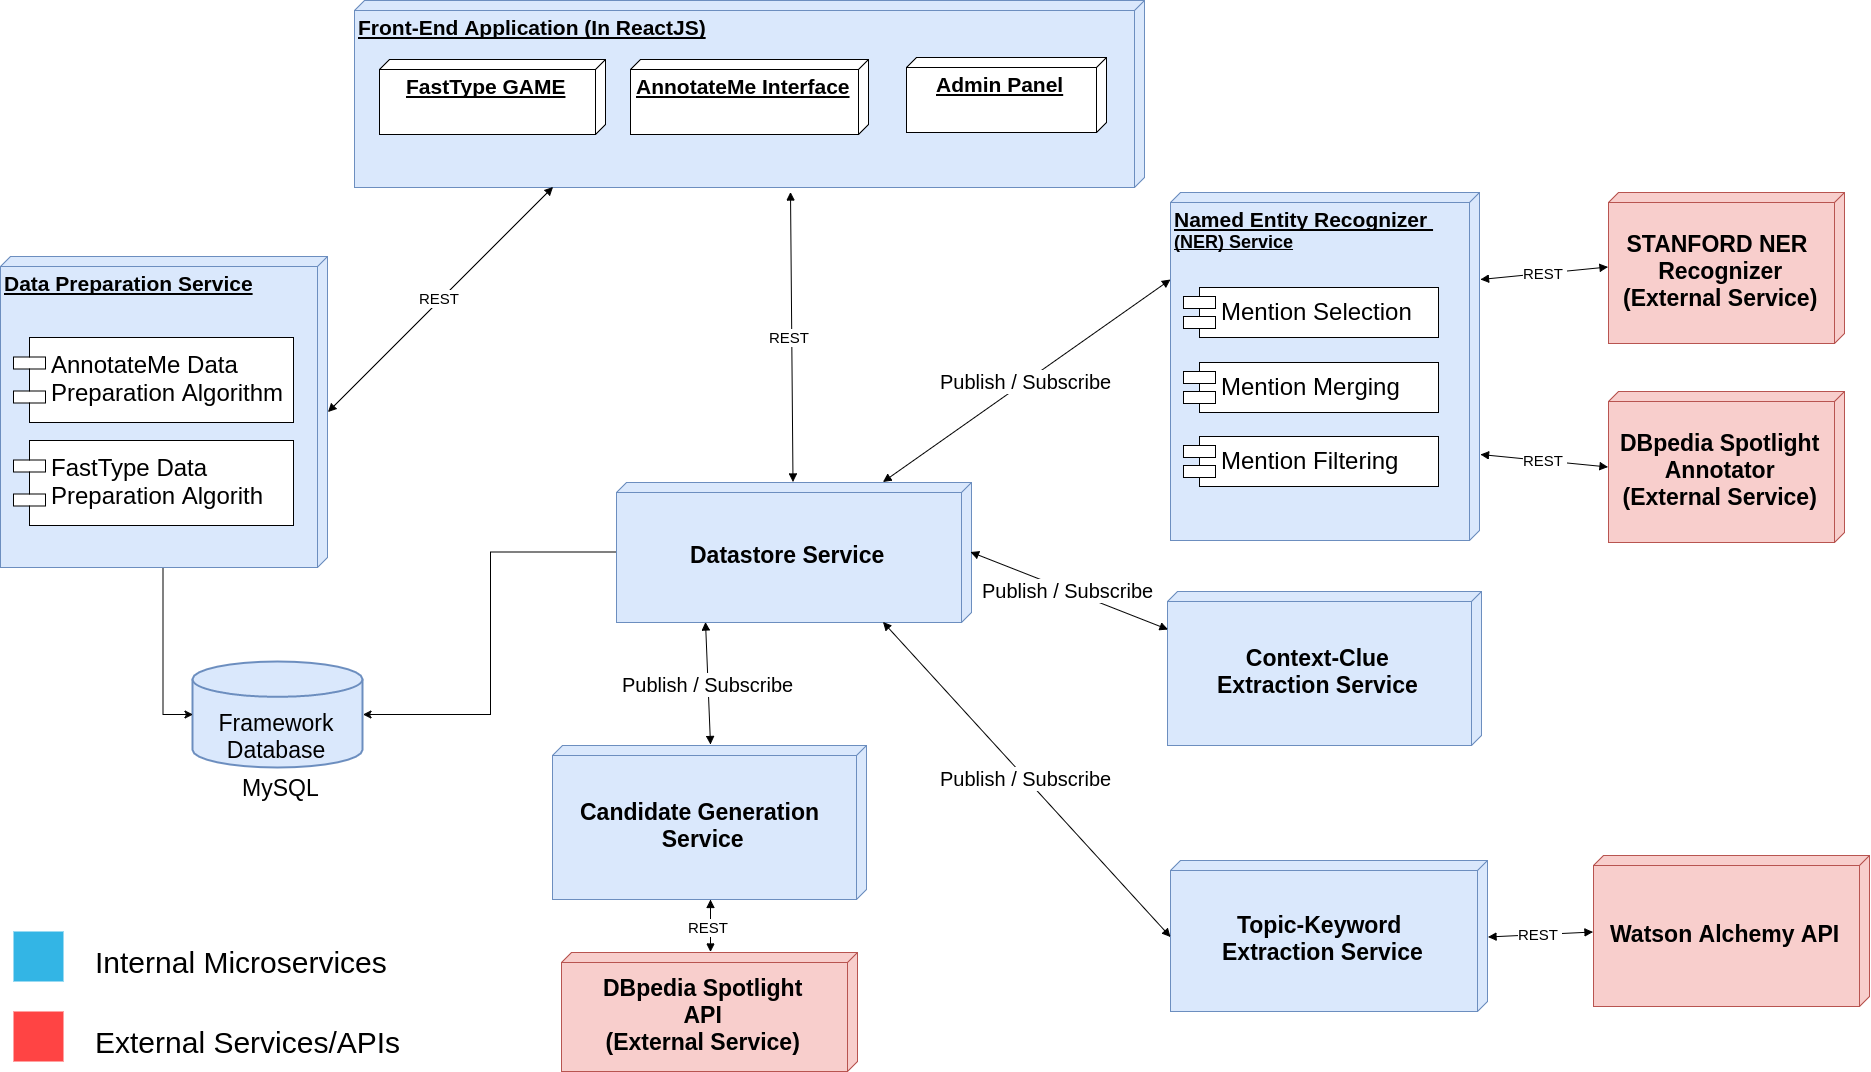
\includegraphics[width=\linewidth]{figures/microservice-architecture.png}
  \caption{Overview of the NED micro-service architecture}
  \label{fig:microservice_architecture}
\end{figure}

Observing the figure above, two different categories can be identified. The internal microservices (boxes highlighted with blue) are services that have been completely implemented from scratch. On the other hand, the external microservices (boxes highlighted in red) are external open source services that have been used by our framework to perform actions which were out of scope of this study. Among the external services, \textit{Stanford NER Recognizer} was the only external service that was not available as an online service offering API calls to perform the corresponding actions. A detailed explanation of the NER microservice is provided later in section \ref{framework:architecture_NER}.

%Communication Infrastructure
In a microservice architecture, a key factor that differs this architecture from other design patterns is the lightweight communication/messaging infrastructure. In our framework, we have utilized two different communication protocols, namely, Synchronous Messaging (\ac{rest}) and Asynchronous Messaging (\ac{amqp}). In cases where immediate response is required from a service to another, RESTful request/response API calls have been used to exchange information. We have tried to adhere to the fundamental rules of the RESTful messaging protocols where every functionality of the service is represented with a resource and operations carried out on top of these resources. As illustrated in Figure \ref{fig:microservice_architecture}, the front-end service which contains the admin panel, AnnotateMe Interface and Fastype Game communicate synchronously with the data preparation service and data store service. In addition to the front-end service, all external services are invoked using synchronous REST API calls since our internal microservices are not able to perform any internal actions unless the response from the external service is acquired. A complete documentation of the REST API calls implemented in the data store and data preparation services are available in Appendix \ref{appendix1:RESTDOCsec}.

Some of the services that compose the framework usually have a longer processing time compared to others because of the underlying complexity and the calculations that need to be performed. In these cases, it is more practical to use asynchronous messaging protocols without having to freeze the overall process as a consequence of one service which takes longer to complete. The publish and subscribe asynchronous message communication model was used for this purpose. More specifically, RabbitMQ \footnote{RabbitMQ Documentation Page \url{https://www.rabbitmq.com/documentation.html}} was used as the underlying lightweight message brooker based on \ac{amqp} (Advanced Message Queue Protocol). To see the different publishing and subscription routes that build the asynchronous communication infrastructure of the framework, see Appendix \ref{appendix1:AMQPDOCsec}.

%Conteinarization - Docker 
When designing a microservice architecture, among the many important design patterns that distinguish this architectural style from others is the deployment process. The deployment of microservices plays a critical role and when it comes to microservice architecture, the following key requirements have to be satisfied \cite{dzone}:
\begin{itemize}
    \item The ability to deploy/un-deploy independently each service
    \item It must be able to scale at each microservice level (as some services may experience more trafic than others)
    \item The ability to build and deploy microservices quickly
    \item In case one microservice fails to execute, other microservices should not be affected by this failure
\end{itemize}

To comply with the above mentioned requirements, Docker\footnote{Docker Documentation Page \url{https://docs.docker.com/}} was considered as the best microservice deployment solution. Docker is a containerization tool that lets developers and system administrators deploy self-sufficient application containers in Linux environments \cite{dzone}. Deploying a microservice into a docker container is as easy as writing a 5 line script. The steps involved to deploy an application into a docker container are as follows \cite{dzone}: 
\begin{itemize}
    \item Packaging the microservice as a Docker container image (usually by writing a script)
    \item Deploying each service instance as a container
    \item Linking containers with each other so that they are able to communicate (this is done automatically by Docker)
    \item Scaling is done by deploying many instances of the same container
    \item Building, deploying and starting a microservice is relatively fast as Docker uses containers instead of virtual machines (which is much slower compared to containers)
\end{itemize}

%Technology Stack - NodeJS, ReactJS, Mysql db
In terms of technology stack used to implement the microservice framework, the latest web technology tools have been utilized. In addition to the previously mentioned tools used for communication and deployment, the actual microservice applications framework has been implemented using NodeJS\footnote{NodeJS \url{https://nodejs.org/en/docs/}} as a back-end programming language, whereas for the front-end implementation we used ReactJS\footnote{ReactJS \url{https://facebook.github.io/react/}}. The combination of NodeJs and ReactJS has proven to be very efficient in terms of development speed, performance, agile development support and the incredible fast rendering capabilities which is very helpful during development and debugging of the application. As for the data storage, MySQL relational database has been used in our framework. 

Figure \ref{fig:workflow} illustrates the complete workflow of the framework. We use this illustration as a reference when describing the different services composing the framework in the following sections.


\begin{figure}[]
  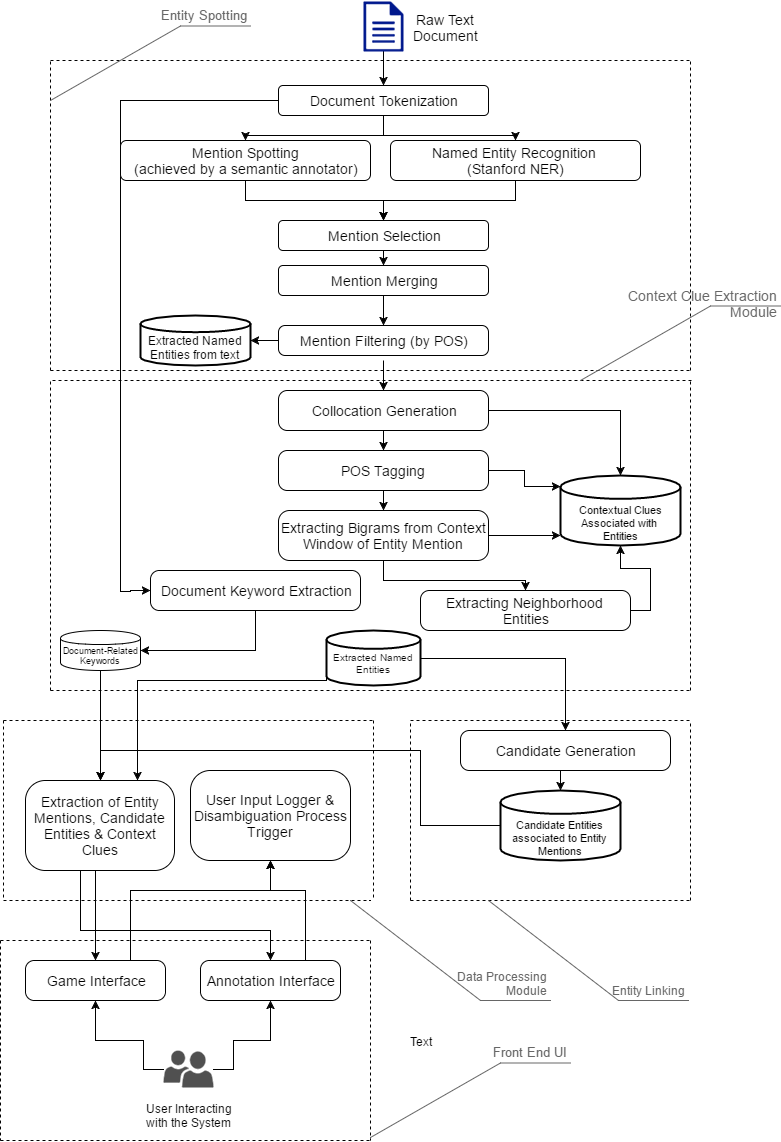
\includegraphics[width=\linewidth]{figures/workflow-diagram-v4.png}
  \caption{Overview of the complete workflow of the NED Framework}
  \label{fig:workflow}
\end{figure}


\newpage 
\subsection{Named Entity Recognition (\ac{ner}) Service}
\label{framework:architecture_NER}
The disambiguation process is initiated by uploading a raw text document through the admin panel which issues an API call to the data store service. The data store service persists the content of the document into the database and proceeds by publishing a \textit{named entity recognition} message which in turn is subscribed by the NER microservice. The published message contains all the textual content of the uploaded document. As can be seen in Figure \ref{fig:workflow}, the NER microservice starts by tokenizing the textual content of the document. A NodeJS implementation of a tokenizer has been used for this purpose \footnote{See Node Tokenizer \url{https://www.npmjs.com/package/tokenize-text}}. The tokenization process converts the text content into an array of words, sentences, characters or any other desired way. We use the tokenizer to split up sentences and individual words. 

The whole named entity recognition procedure has been inspired by \cite{39}, as they achieve very high levels of accuracy and significantly outperform state-of-the-art named entity recognizers. However, the implementation of the \ac{ner} service by Chabchoub et al. \cite{39} was carried out as part of the OKE Challenge 2016 and we were not able to find any open source code that could be integrated into our framework. Based on the information the authors provide in their publication, an attempted was made to reproduce the algorithms used in the recognition module in order to achieve similar performance levels as reported in their publication \cite{39}.

Stanford \ac{ner} \cite{standfordNER} has been used as a named entity recognizer in combination with Dbpedia Spotlight \cite{dbpedia} as a semantic annotator. Both (as external services) recognize the entities in the textual content and return a list of all the recognized entities. When comparing the results of each service, entity overlapping was observed. To be able to solve this, a selection algorithm is implemented in order to select the best entity out of both lists. The logic of the selection algorithm is keeping the longest mention and dismissing the short one. Lets take an illustrative example from the sentence below: 

\begin{quote}
\textit{"The State University of New York at Cortland celebrated its 149th anniversary this year."}
\end{quote}

In this example, Spotlight annotates \textit{State University} and \textit{New York}
 separately, whereas Stanford NER recognizes it as a single entity, namely, \textit{State University of New York}. The mention selection algorithm makes sure that the former is discarded and the later is kept. 
 
 However, even after the mention selection algorithm, it is not guaranteed that the correct entities have been identified. From the example sentence, in fact, the correct entity mention is \textit{State University of New York at Cortland}. In order to achieve this, the mention merging algorithm is performed. As explained by \cite{39}, given two named entities in close proximity, the algorithm will try to expand it to cover the next entity mention. The constraints checked by the algorithm to permit the expansion (avoiding pitfalls such as merging two legitimate different entities) have been described in detail by Chabchoub et al. \cite{39}. 
 
 The last step, before the entities are persisted into the database, consists of applying the mention filtering algorithm to the list of identified entities. The mention filtering algorithm uses a standard Part-of-Speech tagger for getting linguistic information for each entity. Accordingly, all entities that contain verbs are removed from the list, thus, filtering out incorrectly recognized entities \cite{39}. 
 
 The final result of the \ac{ner} micro-service contains a list of \textit{selected}, \textit{merged} and \textit{filtered} entities. The \ac{ner} service finalizes its process by publishing a \textit{named entity persist} message which is subscribed by the data store service that does the actual persisting of the entities into the MySQL database.

\subsection{Context Clue Extraction Services}
%Bigrams 
During the background chapter we emphasized the importance of context and how much it can affect the disambiguation accuracy for both, automatic and manual annotation systems. Referring back to the work-flow presented in the diagram in Figure \ref{fig:workflow}, contextual clues are extracted by following a three step process.

The process starts by removing all stop words in the sentences where the entity mentions are part of. After the stop words have been removed from the sentences, the \textit{collocation generation algorithm} is performed on those sentences. Collocations, according to Colson et al. \cite{52} represent the occurrence of two or more words within a short proximity between each other in text. They also argues that collocations are more likely to occur as fixed expressions such as compound nouns, proper nouns, idioms, noun-adjective combination, adjective-noun combination, verb-noun, well known song or film titles. The collocation generation algorithm follows these principles when deciding to keep a collocation from the sentence or not. Since we are dealing with analysis of grammatical structures in the sentence, part-of-speech tagging is a crucial step to be performed at this stage. 

After having extracted all potential collocations from the sentence provided as input data to the service, the next step is to associate these collocations as contextual clues to each and every entity. However, not every identified collocation within the sentence can be a useful context clue for the entity that is also part of that sentence. Previous studies have used a context window size of 4, which means that they take four preceding and four subsequent words from the sentence where the target entity occurs \cite{35}. The number 4 has been chosen because the accuracy of sense resolution does not improve when more than 4 words around the target word are considered. However, recent studies argue that the context windows size around the ambiguous target entity is dependent on the nature of the word itself \cite{35}. Our solution to this problem is increasing the context window size depending on how ambiguous the target word is. The ambiguity of a target entity is defined by the number of potential candidates extracted from the \ac{kb}. The more candidates are generated for the target entity, the higher the level of ambiguity. We believe that this represents an accurate metric on deciding the context size of the target entity. 

Since collocations can be a combination of more than two words, we have decided to keep only collocations that are composed of two words (i.e. bigrams). This decision is influenced on the findings acquired by Mihalcea and Rada \cite{36}. They observed that in terms of words in context, bigrams seem to be more effective than simple keywords and other combinations larger than two.In addition to the collocations which are considered as clues to help summarize the context in which the target word occurs, neighbour entities also also fall into this category. Since the algorithm has information on the exact position of each entity in the sentence (by maintaining a starting and ending index), we are able to decide which (other) entities are in close proximity to the target entity. Usually all identified entities that are part of the same sentence as the target entity are considered as neighbor entities. In some cases, when the sentence is short, the algorithm looks for neighbor entities in the preceding and subsequent sentences. The algorithm maintains a constraint on which it bases its logic whether to consider keeping or discarding a neighbor entity for the target entity. The constraint is basically a calculated word distance between the target entity and all other potential neighbor entities. 

After the local contextual clues have been extracted by our internal microservice, the last step is the extraction of document keywords. Document keywords are used to represent the theme or topic of the document, and might help in the disambiguation process in addition to local contextual clues. In this stage, Alchemy API is queried which extracts the most important keywords from a document. These keywords are associated as context clues to all identified entities in the same document whereas local context clues are distinct from one entity to another. Figure \ref{fig:context-clue} illustrates an example of a paragraph and the corresponding results after running the context clue extraction service. In this example, the target entity for which the context clues are to be associated is highlighted in red. The legend illustrated as a table in the example figure explains the meaning of the different colors. In cases where the words are underlined and highlighted with different colors, it means that the word combination has multiple purposes. For example "New York" from the illustrative paragraph in Figure \ref{fig:context-clue} is considered a neighbor entity to G1 (the target entity) in addition to being a keyword that contributes to understanding the meaning of the complete paragraph.


\begin{figure}[]
  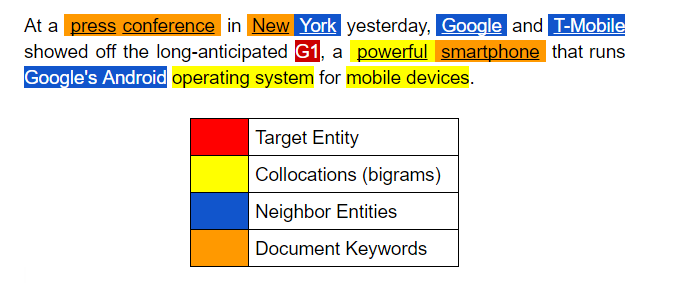
\includegraphics[width=\linewidth]{figures/context-clues.png}
  \caption{An example of a paragraph and the different contextual clues extracted from the service}
  \label{fig:context-clue}
\end{figure}

\subsection{Candidate Generation Service}
Dbpedia Spotlight is the semantic annotator which is queried by the \textit{Candidate Generation Service} to extract DBpedia candidates for a specific entity mention. No special logic has been applied in this service and therefore, the results retrieved after querying Dbpedia Spotlight are persisted into our system without additional modifications to the original data.

Dbpedia Spotlight \cite{dbpedia} performs the disambiguation process by pre-ranking entity candidates for each surface form spotted in the text. A combination of a prior score and a contextual score is calculated in order to determine which candidate entity is the most relevant. The prior score represents an estimation of how often the surface form is used as an anchor in a Wikipedia hyperlink that points to the entity page \cite{39}. Whereas the context score makes use of the context of the phrase (usually a window of words around the phrase) and the context of each candidate entity (calculated internally by Spotlight). When querying highly ambiguous entities such as "Paris" which can have over ten target candidates, only the best 8 are fetched to be evaluated. According to a user study conducted by Bontcheva et al. \cite{33}, participants gave feedback that having more than 8 options to choose from is associated with high cognitive load which results in immediately exhausting users. In addition to the maximum number of 8 candidate entities, we provide a last option called "none of them" in case the Spotlight was not able to fetch the correct candidate in the list.

During the experimental user study we observed that Spotlight was not able to provide the correct candidate entity for many entity mentions. Therefore we experimented with providing different context window sizes to the annotator to see if the performance changes. First we queried Spotlight by providing only the entity itself without any other contextual information. Second, the contextual clues extracted by our microservice were put in a sentence together with the target entity with clues located prior and after the target entity (based on where the clues were located on the original sentence). Finally, the original sentence where the target entity is part of, was used as context and sent as query parameter to Spotlight. We report in the results section of this chapter that the differences in performance between the three groups is relatively small and does not assure statistical significance.

\subsection{Data store \& data preparation service}
To assure the control and consistency of data being processed by the different microservices composing the framework, the \textit{Data-Store Service} was designed to be the only entry point to which the data could be manipulated. The service provides endpoints for accessing and manipulating the information residing on the database as a means of API calls and asynchronous message inquiries. It also serves as an information provider to the admin panel in the front-end application and also subscribes to different message routes such as: persisting named entities recognized from \ac{ner} microservice, persisting context clues and associating the generated candidate list to all registered entity mentions in the database. Besides subscribing to these message routes, the \textit{Data-Store Service} is the service endpoint that manages the complete asynchronous messaging infrastructure.

On the other hand, the \textit{Data-Preparation Service}, as the name implies, prepares the data for the AnnotateMe Interface as well as for the Fastype Game. Similar to the Data-Store Service, it has direct access to the database information with only one specific permission: reading (i.e. querying and retrieving information from the database). Therefore, for the sake of centralization and control of data, the Data-Preparation Service is considered as a read-only service with regards to the database access.

A unique feature implemented in the data preparation service is, as we like to call it, the \textit{disambiguation trigger}. This feature is responsible for resolving a specific entity mention (deciding which candidate represents the correct link for the target entity) when enough annotation data from the human annotators are accumulated. Since the most usual use-case scenario includes non-expert human annotators performing the validation process by either using the AnnotateMe Interface or the Fastype game, assuring quality of annotations is reached through redundancy. The level of redundancy maintained in the data preparation service is based on constraints proposed by Snow et al. \cite{32}. They conducted an experiment where they evaluated the quality of non-expert annotators in comparison with expert annotators. Their results indicate that on average it requires 4 independent non-expert annotations to achieve the equivalent ITA of a single expert annotator. Therefore, the disambiguation trigger is triggered when 4 independent annotations (having the same candidate as the selected option) have been accumulated for a specific entity mention. After an entity has been resolved, it will no longer show up on the interface for validation. The resolving step is done by the \textit{Data-Preparation Service} which initiates a REST API call to the \textit{Data-Store Service} in order to update the information on the databse.

%Order effects
A final element that is taken care by the \textit{Data-Preparation Service} is the ordering of candidates presented to human annotators. In a study conducted by Duarte et al. \cite{34}, they argue that in search engines, web users expect the best answer to be in the first or second position. This type of expectation represents potential bias on the results assessing the behaviour of annotators. After performing some user studies, they conclude that search result selection behaviour is influenced by ranking, with users showing tendency to select higher ranks without exploring other alternatives. To avoid having this situation in our experiment, we encourage users to explore all the candidates presented to them before making a decision. The encouragement is done by providing short descriptions for each candidate on the interface. Additionally, we avoid the chance of making users form assumptions about potential candidates being ranked higher in a list by completely randomizing the process of candidate positioning. Random positioning of alternatives instead of ranking has proven to be much more effective in encouraging users to explore all available alternatives instead of making blind decisions \cite{34}.


\newpage
\subsection{AnnotateMe Interface}

\begin{figure}[]
  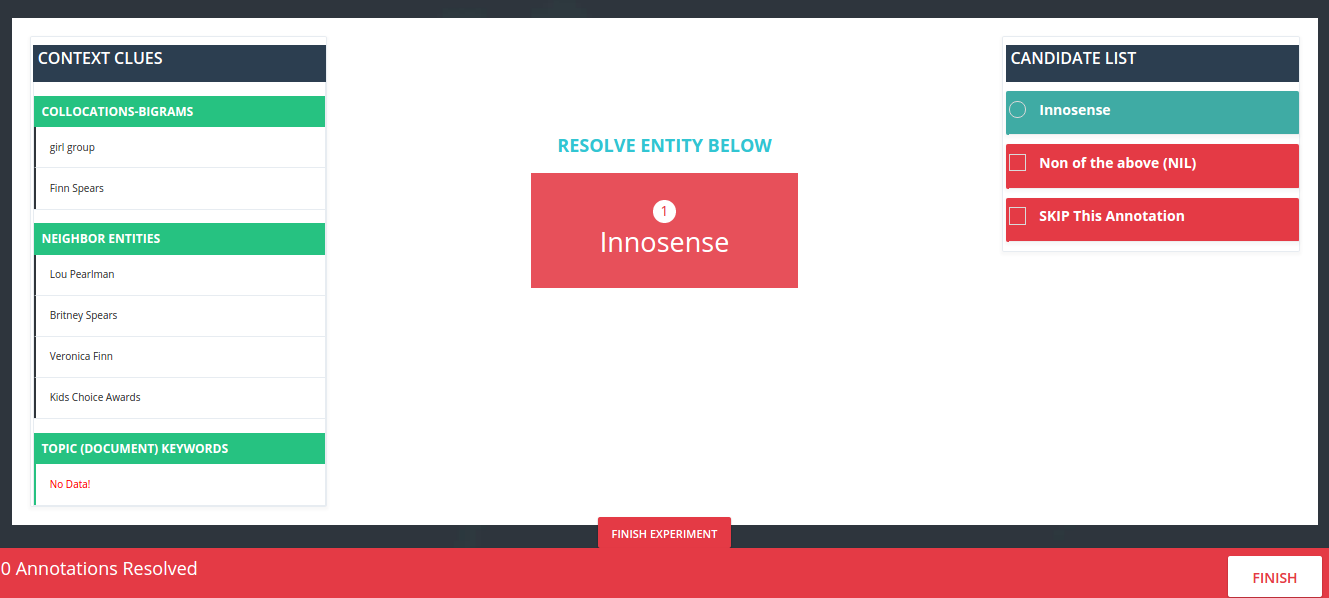
\includegraphics[width=\linewidth]{figures/annotateme-interface.png}
  \caption{The AnnotateMe Interface used to conduct the first experiment for validating the links generated by the NED Framework}
  \label{fig:annotateme-interface}
\end{figure}

During the implementation of the AnnotateMe Interface, we tried to come up with a simple UI and UX design of the interface in order to maintain low levels of complexity and avoiding confusion. Some of the design patterns identified by Hinze et al. \cite{15} necessary for non-expert users to annotate the presented content have been explored while implementing the annotation interface. These design patterns include:
\begin{itemize}
    \item Intuitive User Interface - an interface that is easy to grasp with actions that require minimal effort to discover and perform
    \item Simple Vocabularies - the current architecture of the framework provides annotations of entities within the categories of Organization, Location and People which are genuinely simple in nature.
    \item Focus on user task - The interface does not have any disruptive features or elements that would shift the focus of the annotator from its main task, that is, resolving the presented named entity.
\end{itemize}

% Quality check
According to Bontcheva et al. \cite{33} the single most influential part of any linguistic annotation exercise is the annotators ability to understand and conduct the annotation task. In order to achieve this, the guidelines and tools provided by the annotation interface play a major role in controlling such behavior. Presenting the user with simple, short guidelines that include examples and specific instructions on how to perform certain actions is very helpful. Additionally, having a clean interface is of utter most importance which contributes to an intuitive interaction during the annotation process. \cite{33} 

Figure \ref{fig:annotateme-interface} represents the design of the AnnotateMe Interface used for conducting annotations with non-expert users. The target entity mention to be resolved is presented in the middle of the page and attracts the users focus by reflecting its importance in the overall task. The contextual clues are presented to the right hand side of the interface and are grouped based on their origin of extraction. The right hand side of the interface is reserved for the candidate list. Each candidate can be expanded by clicking on its name. The expanded candidate provides the user with additional information that describes the meaning of the candidate (usually a short description). The two last options in the candidate section highlighted with red provide some degree of freedom to the user in case they are unfamiliar with the entity or when they think that the correct candidate is not provided in the list. These two options being discussed are: \textit{Non of the above(NIL)} and \textit{Skip this annotation}. The interface presented in Figure \ref{fig:annotateme-interface} has been used to conduct the first experiment which will be described in detail in the next upcoming section.
\newpage
\section{Methodology}
\label{framework:methodology}

The implementation of the Named Entity Disambiguation Framework with all its underlying microservices represent the tool which is used to study and answer the first two research questions. The majority of the implementation patterns and algorithms are based on theoretical background and reviewed literature on the respective field. In absence of open source code, the \ac service has been implemented as a reproduction of the work conducted by Chabchoub et al.~\cite{39}. However, without actual contribution of human annotators by participating in a user study, the answers to the research questions would not have been resolved. The first experimental user study has been conducted in order to get detailed insights on how well the information processed and presented to human annotators would contribute to generating annotation data. The reason that two user studies were conducted during this research work was to measure the engagement and playfulness of the game when compared to a standard, non-gamified interface for named entity disambiguation. Data from both experiments have been used to analyze and compare the different characteristics in order to draw on conclusions that we initially set to achieve. Regardless, this methodology section represents all the necessary information needed to successfully conduct the first experiment and describe the techniques and methodologies used to analyze the results.

%Datasets 
In order to conduct the annotation experiment by using the designed AnnotateMe Interface, an annotation data gathering process was conducted beforehand. In absence of linguistic and expert annotators to construct a gold standard which would have been used for assessing the quality of annotations, we decided to use already existing datasets, namely, Spotlight and KORE50 datasets \cite{datasets-ex1}. The first dataset contains documents from news articles whereas the second one contains short articles extracted from various domains. KORE50 is known by the NLP experts as a dataset characterized with a highly ambiguous nature. Table \ref{tab:experimentone_dataset} summarizes all the different entity types that are recognized in each dataset used in our evaluation experiment. As observed from the table, both datasets are composed mostly of entities in the three main categories: Organization, Location and People. The table was originally reported by Steinmetz et al. \cite{datasets-ex1}, and during the time of their writing, some of the entity mentions recognized in the dataset did not have a \ac{kb} representative. However, it has been mentioned that the information in \ac{lod} is continuously increased by researchers contributing with new datasets and extending existing ones, the ratio of mentions and entities from both datasets is likely to be more equalized now\footnote{The number of entity mentions recognized in the text having a corresponding \ac{kb} representative is increased.}. However, the analysis and results presented in the next section are up-to-date and take into consideration the latest versions of KROE50 and Spotlight datasets. 

\newpage
% Table generated by Excel2LaTeX from sheet 'Sheet1'
\begin{table}[htbp]
  \centering
  \caption{Distribution of entity types for Spotlight and KORE50 \cite{datasets-ex1}}
    \begin{tabular}{|l|rr|rr|}
    \toprule
    \multicolumn{1}{|c|}{\multirow{Class}} & \multicolumn{2}{c|}{Spotlight } & \multicolumn{2}{c|}{KORE50} \\
\cmidrule{2-5}          & \multicolumn{1}{l|}{Entities} & \multicolumn{1}{l|}{Mentions} & \multicolumn{1}{l|}{Entities } & \multicolumn{1}{l|}{Mentions} \\
    \midrule
    Total & 249   & 331   & 130   & 144 \\
    Agent & 1.40\% & 2.70\% & 66.90\% & 70.80\% \\
    -Organization & <1\%  & <1\%  & 19.40\% & 5.30\% \\
    --Company & <1\%  & <1\%  & 9.20\% & 9.70\% \\
    --Sports Team & -     & -     & 7.70\% & 6.90\% \\
    ---Socer Club & -     & -     & 7.70\% & 7.90\% \\
    -Person & 2.00\% & 2.40\% & 48.50\% & 51.40\% \\
    --Artist  & -     & -     & 17.70\% & 18.80\% \\
    ---MusicalArtist & -     & -     & 17.70\% & 18.80\% \\
    --Athlete & -     & -     & 6.90\% & 8.30\% \\
    ---SoccerPlayer & -     & -     & 5.40\% & 6.30\% \\
    --OfficeHolder & <1\%  & <1\%  & 4.60\% & 4.20\% \\
    Disease & 1.60\% & 1.20\% & -     & - \\
    EthnicGroup & 1.20\% & 1.80\% & -     & - \\
    Event & 1.20\% & <1\%  & -     & - \\
    Place & 10.40\% & 10\%  & 10.80\% & 10.40\% \\
    -Architectural Structure & 2.00\% & 1.50\% & 3.10\% & 2.80\% \\
    --Infrastructure & 1.60\% & 1.20\% & <1\%  & <1\% \\
    -PopulatedPlace & 7.20\% & 7.60\% & 5.40\% & 5.50\% \\
    --Country & 3.60\% & 3.30\% & -     & - \\
    --Region & <1\%  & <1\%  & -     & - \\
    --Settlement & 2.40\% & 3.30\% & 3.80\% & 3.50\% \\
    ---City & 1.60\% & 2.10\% & 2.30\% & 2.10\% \\
    Work  & <1\%  & <1\%  & 6.20\% & 6.30\% \\
    -MusicalWork & <1\%  & <1\%  & 3.10\% & 3.50\% \\
    --Album & <1\%  & <1\%  & 3.10\% & 3.50\% \\
    \bottomrule
    \end{tabular}%
  \label{tab:experimentone_dataset}%
\end{table}%

%recruiting participants
The participants who took part in the annotation experiment were invited through emails and social media. On the invitation message sent to all participants, a short and abstract description of the idea behind the experiment was provided. It is important to note that payment incentives and any other type of incentive which would degrade the voluntary participation of the user were avoided, thus assuring a complete voluntary participation without any beneficial intentions. As a result, 30 participants showed up and successfully completed the experiment.

The experiment was conducted in closed group rooms at the university campus in order to make sure that the participant was not being distracted while performing the experiment. Before starting to perform the actual annotations, the participants were presented with a consent form which explained the nature, purpose and intentions of the experiment. Participants were also fully aware that the participation was anonymous and voluntary and withdrawal from participation was possible at any time. The consent form for the first experiment is provided in Appendix \ref{appendix1:annotatme}.

On average, the duration of a single experiment session was about 25 minutes long. We also asked the participants to fill in a pre-questionnaire to gather demographic information about them as well as questions that assessed the level of expertise of each participant in the field of semantic web and natural language processing. In order to avoid potential biases on the results, we made sure that participants had moderate to native skills in English. We report on the demographic data of participants in the next section whereas the questions provided in the pre-questionnaire are presented in Appendix \ref{appendix1:annotatme}.

The non-expert nature of participants and the time constraints on the duration of an experiment session for each participant was the main reason for recording an instructional video to be presented to each participant before starting the actual annotation task. This video was essentially a replacement for an introductionary interface that is usually implemented for such experiments. During the 4 minute demonstrative video, we demonstrated to the participants how the interface is used and the purpose of each elements towards the general idea of annotating. After having read the consent form, filled in the pre-questionnaire and watched the demo video, the participants proceeded in doing the annotations for 15 minutes. However, the experimenter did not provide upfront information on how many annotations had to be performed. After the estimated 15 minutes elapsed, the participants were instructed to either finish the experiment or continue do more annotations This was a technique we used for measuring the level of enjoyment that participants had towards the interface. After the participant free-willingly\footnote{A free-will annotation is an annotation performed by a participant after being aware that the experiment was completed. This is a metric to measure the attractiveness of and engagement with the interface as perceived by the participant.} decided to finish the experiment, he or she was asked to fill in a post-questionnaire. The post-questionnaire contained questions with the purpose of assessing the quality, usability and engagement level of the interface. We report on the results of the post-questionnaire in the next section. The questions provided in the post-questionnaire can be found in Appendix \ref{appendix1:annotatme}.

% Assessment methodologies, f-measures, annova analysis, accuracy calcuations (for NER and Automatic annotator)
For assessing the performance of the framework in terms of entity recognition, user annotation quality and agreement level, we used metrics such as precision, recall, f-score and one way ANOVA analysis of variance. These assessment methodologies are commonly used in entity linking systems \cite{12}. Furthermore, to be able to assess the performance of our approach with state-of-the-art frameworks we have used a generic benchmark called GERBIL  originally developed by Usbeck et al. \cite{40}. GERBIL is a comparison tool for easily discovering the strengths and weaknesses of your implementation with respect to the state of the art in named entity disambiguation. The tool is open source and is an extensible framework that currently supports 9 different annotations on 11 different datastes within 6 different data types (recognition, disambiguation, linking etc). We report on the results of our framework with respect to the state-of-the-art annotators offered by GERBIL for Spotlight and KORE50 datasets. 

% Justify why we have used the following methodology. Why is it best fit for our study and answering our research questions

% Likely sources of BIAS
Concerning limitations and potential sources of bias, the methodology we used for our research study can be considered partially immune. For the sake of reproducability, we need to note that the participants who were invited through emails and social media were within the scope of the university campus. Consequently, one might argue that they might have been biased to participate in the experiment. Since this was seen as the only way of recruiting the participants in the pressure of time and space, we account this as a potential source of bias and address as a limitation of the recruitment methodology. However, we assure consistency with regard to participant recruitment since the same approach was used to recruit participants for the second experiment as well. Therefore, in case the results indicate increased engagement and motivation by using the game compared to the plain interface, we are able to claim that the improvements are acceptable since we remain consistent in the methodology. 

%Hypothesis 
\paragraph{Hypothesis}
The aim of the first experiment is to find out whether the implemented framework supports qualitative annotations by non-expert annotators. Therefore, we hypothesize that:

\begin{itemize}
    \item H1.1: By implementing the complete entity disambiguation pipeline as a framework, non-expert users will be able to perform annotations with a quality compared to expert annotators!
    \item H1.2: Short contextual clues are preferred towards complete sentences or paragraphs and as such provide sufficient information to make correct disambiguations! 
\end{itemize}



\newpage
\section{Results}
\label{framework:results}
The reason for performing the first experiment with the AnnotateMe Interface was to find out whether our approach of formulating and presenting the annotation data to a non-expert annotator for validation would result in creating high quality annotations. During this experiment we have also tested the performance of our NER service to see how well the recognition task is performed in addition to testing the performance of DBpedia Spotlight as the utilized automatic annotator. Below we report on the different aspects of the experiment.

\subsection{Participants}
The non-expert annotators who took part in the first experiment can be characterized as moderate users of text processing tools who have (on average) moderate experience with tagging of textual documents. Please note that tagging was explained to the users as the process of assigning a label or a textual description to a picture, video or categorizing a document. In some cases, the easiest way of explaining the tagging process to a participant was taking the concept of a \textit{hashtag} as an analogy to tagging. However, a \textit{hashtag} provides a higher degree of freedom since the tagging process is open while in our case the user is presented with options to choose from. Regardless, they both share the same conceptual idea. These questions were used to obtain a rough idea about the informal level of expertise of each participant in text processing respectively.

The average annotator was a 25 years old male student studying in the field of Computer Science with a good familiarity of text processing tools, moderate experience with tagging, acceptable level of familiarity with semantic web concepts who considered himself as above average when asked for his English language skills. Figure \ref{fig:ex1-preqestionnaire} presents the results of the questions asked to the participants during the pre-questionnaire. 

\begin{figure}[]
  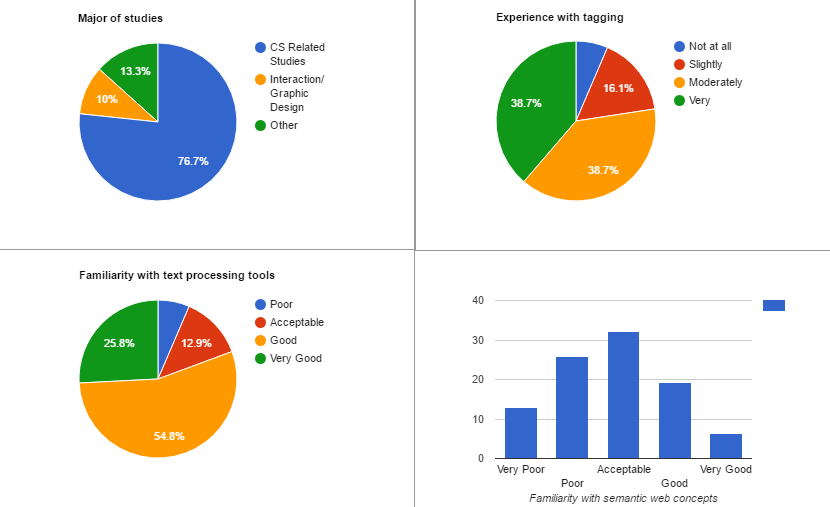
\includegraphics[width=\linewidth]{figures/experiment1/ex1-prequestionnairestats.PNG}
  \caption{Participant Statistics for Experiment 1}
  \label{fig:ex1-preqestionnaire}
\end{figure}

\subsection{NER Performance}
It has been mentioned earlier that the algorithms implemented in our \ac{ner} microservice are not novel solutions as opposed to the state-of-art. We attempted to reproduce the same algorithms used by \cite{39} since at the time of writing, their approach performed best compared to any other state-of-art \ac{ner} algorithms and tools. However, in absence of open source code, we tried to implement the service as similar as possible based on the information the authors provided in their white paper submitted at the OKE Challenge 2016 \cite{39}. As we can see from Table \ref{tab:ex1-nerperformance}, our framework performs significantly better than all the other automatic annotators for the KORE50 dataset, whereas for the spotlight we observe a slightly better improvement. Please note that we used GERBIL Benchmark \cite{40} to get the values for the other annotators whereas for our framework we calculated the same measures as explained by the benchmarking tool. 

% Table generated by Excel2LaTeX from sheet 'Sheet2'
\begin{table}[htbp]
  \centering
  \caption{NER Performance of automatic annotators in two datasets compared to our framework}
    \begin{tabular}{|l|ccc|ccc|}
    \toprule
    \textbf{-/Dataset} & \multicolumn{3}{c|}{\textbf{Spotlight Dataset}} & \multicolumn{3}{c|}{\textbf{KORE50 Dataset}} \\
    \midrule
          & \multicolumn{1}{l|}{\textbf{Precision}} & \multicolumn{1}{l|}{\textbf{Recall}} & \multicolumn{1}{l|}{\textbf{F-Score}} & \multicolumn{1}{l|}{\textbf{Precision}} & \multicolumn{1}{l|}{\textbf{Recall}} & \multicolumn{1}{l|}{\textbf{F-Score}} \\
    \midrule
    \textbf{Babelfy} & 0.22  & 0.18  & 0.19  & 0.55  & 0.55  & 0.53 \\
    \textbf{Dbpedia} & 0.61  & 0.34  & 0.43  & 0.73  & 0.23  & 0.27 \\
    \textbf{AIDA} & /     & /     & /     & 0.64  & 0.53  & 0.57 \\
    \textbf{Dexter} & 0.71  & 0.27  & 0.38  & 0.27  & 0.15  & 0.18 \\
    \textbf{AnnotateMe } & \textcolor[rgb]{ 1,  0,  0}{\textbf{0.69}} & \textcolor[rgb]{ 1,  0,  0}{\textbf{0.42}} & \textcolor[rgb]{ 1,  0,  0}{\textbf{0.49}} & \textcolor[rgb]{ 1,  0,  0}{\textbf{0.87}} & \textcolor[rgb]{ 1,  0,  0}{\textbf{0.8}} & \textcolor[rgb]{ 1,  0,  0}{\textbf{0.82}} \\
    \bottomrule
    \end{tabular}%
  \label{tab:ex1-nerperformance}%
\end{table}%

Our intentions were to see how good our framework performs when dealing with entities that have a very high ambiguous nature (KORE50 Dataset) but also with entities that have moderate levels of ambiguity (Spotlight Dataset). However, the number of entities present in each dataset was relatively big and resolving all of those entities using the framework would require running the experiment for longer periods. Therefore we used only a subset of documents from the Spotlight Dataset wheres for the KORE50 dataset we used all the available documents. For reproducability reasons, the following documents from the Spotlight dataset were considered: Arts1, Business1, Fashion1, Medicine1, Music1, Privacy1, Science1, Sports1, Travel1 and Travel2. The complete dataste is available online at the GERBIL website \footnote{\url{http://aksw.org/Projects/GERBIL.html}}. The total number of recognized entities by our NER microservice was 208 with 77 being entities recognized from the Spotlight dataset and 131 entities recognized from the KORE50 dataset.


\subsection{Annotation Quality and Performance}
Among the 208 total recognized entities by our \ac{ner} microservice, only 82 of them were resolved during the first experiment. It should be emphasized again that for one entity to be resolved we required 4 unique judgements from different participants to agree on one specific candidate for it to be resolved. We measured the performance of the human annotators, DBpedia Spotlight and other automatic annotators on those 82 resolved entities and evaluated whether the candidate associated with the entity was the correct one based on the gold standard. Additionally, since we wanted to see how DBpedia Spotlight (as our utilized automatic annotator) disambiguates entities based on the amount of contextual information surrounding the target entity, we report on three cases, namely: providing only the entity itself without any context information, providing the complete sentence and providing the contextual clues extracted from our framework. 
% Table generated by Excel2LaTeX from sheet 'Sheet3'
\begin{table}[htbp]
  \centering
  \caption{Annotation Results of AnnotateMe Interface and Dbpedia Spotlight Anntator}
    \begin{tabular}{|cc|cc|}
    \toprule
    \multicolumn{4}{|c|}{\textbf{Experiment 1 (Entity Name Only)}} \\
    \midrule
    \multicolumn{1}{|r|}{} & \multicolumn{1}{l|}{\textbf{All Datasets}} & \multicolumn{1}{l|}{\textbf{Spotlight Only}} & \multicolumn{1}{l|}{\textbf{KORE50 Only}} \\
    \midrule
    \multicolumn{1}{|c|}{\textbf{Correct (\%)}} & \multicolumn{1}{r|}{44.57} & \multicolumn{1}{r|}{72.22} & \multicolumn{1}{r|}{32.23} \\
    \multicolumn{1}{|c|}{\textbf{Incorrect (\%)}} & \multicolumn{1}{r|}{55.43} & \multicolumn{1}{r|}{27.78} & \multicolumn{1}{r|}{67.77} \\
    \midrule
    \multicolumn{4}{|c|}{} \\
    \midrule
    \multicolumn{4}{|c|}{\textbf{Experiment 1 (With Sentances)}} \\
    \midrule
    \multicolumn{1}{|r|}{} & \multicolumn{1}{l|}{\textbf{All Datasets}} & \multicolumn{1}{l|}{\textbf{Spotlight Only}} & \multicolumn{1}{l|}{\textbf{KORE50 Only}} \\
    \midrule
    \multicolumn{1}{|c|}{\textbf{Correct (\%)}} & \multicolumn{1}{r|}{51.38} & \multicolumn{1}{r|}{70.37} & \multicolumn{1}{r|}{43.31} \\
    \multicolumn{1}{|c|}{\textbf{Incorrect (\%)}} & \multicolumn{1}{r|}{48.62} & \multicolumn{1}{r|}{29.63} & \multicolumn{1}{r|}{56.69} \\
    \midrule
    \multicolumn{4}{c}{} \\
    \midrule
    \multicolumn{4}{|c|}{\textbf{Experiment 1 (With Context Clues \& Neighbor Entities)}} \\
    \midrule
    \multicolumn{1}{|r|}{} & \multicolumn{1}{l|}{\textbf{All Datasets}} & \multicolumn{1}{l|}{\textbf{Spotlight Only}} & \multicolumn{1}{l|}{\textbf{KORE50 Only}} \\
    \midrule
    \multicolumn{1}{|c|}{\textbf{Correct (\%)}} & \multicolumn{1}{r|}{54.24} & \multicolumn{1}{r|}{66.67} & \multicolumn{1}{r|}{48.78} \\
    \multicolumn{1}{|c|}{\textbf{Incorrect (\%)}} & \multicolumn{1}{r|}{45.76} & \multicolumn{1}{r|}{33.33} & \multicolumn{1}{r|}{51.22} \\
    \midrule
    \multicolumn{4}{|c|}{} \\
    \midrule
    \multicolumn{4}{|c|}{\textcolor[rgb]{ 1,  0,  0}{\textbf{AnnotateMe}}} \\
    \midrule
    \multicolumn{2}{|c|}{\textcolor[rgb]{ 1,  0,  0}{\textbf{Correct (\%)}}} & \multicolumn{2}{c|}{\textcolor[rgb]{ 1,  0,  0}{\textbf{Incorrect (\%)}}} \\
    \midrule
    \multicolumn{2}{|c|}{\textcolor[rgb]{ 1,  0,  0}{\textbf{88.46}}} & \multicolumn{2}{c|}{\textcolor[rgb]{ 1,  0,  0}{\textbf{11.53}}} \\
    \bottomrule
    \end{tabular}%
  \label{tab:exp1-annotatorRes}%
\end{table}%


Table \ref{tab:exp1-annotatorRes} presents the ratio of correctly and incorrectly linked entities by Dbpedia Spotlight. In general, the performance increased after providing more contextual information to the automatic annotator, which is an expected outcome. However, against our expectations, in the case of Spotlight Dataset, the ratio of correctly linked entities decreased after providing additional context information to the annotator. Despite the fact that the difference between the groups is not statistically significant for p < 0.5, it leads us to the assumption that Dbpedia Spotlight requires more content than just short contextual clues in order to make use of their internal techniques for disambiguation such as link probability, commonness, semantic similarity and other vector features relevant to context. Finally, we compare our performance results with other automatic annotators aside from Spotlight and we observe a significant improvement on both datasets. Table \ref{tab:exp1-annotatos-comparison} reports on the F-score of each annotator compared to our framework. 

Additionally, we run one-way Anova analysis of variance between two groups, namely, annotation results performed by non-expert users using the AnnotateMe Interface and results obtained by Dbpeida Spotlight automatic annotator. Statistically significant differences for p = 0.05 are obtained. As a result we claim that the non-expert annotators performed significantly better compared to other semantic annotators with an observed accuracy of 0.92 for the f-measure. Based on these results, the first hypothsis (H1.1) is strongly supported.

% Table generated by Excel2LaTeX from sheet 'Sheet4'
\begin{table}[htbp]
  \centering
  \caption{Comparison of AnnotateMe with other state-of-art semantic annotators}
    \begin{tabular}{|l|r|r|r|}
    \toprule
    \multicolumn{4}{|c|}{\textbf{Precision, Recall, F-Scores (Spotlight \& KORE50 Dataset)}} \\
    \midrule
    \textbf{Annotator} & \multicolumn{1}{l|}{\textbf{Precision}} & \multicolumn{1}{l|}{\textbf{Recall}} & \multicolumn{1}{l|}{\textbf{F-Score}} \\
    \midrule
    \textcolor[rgb]{ .8,  0,  0}{\textbf{AnnotatMe}} & \textcolor[rgb]{ .8,  0,  0}{\textbf{0.95}} & \textcolor[rgb]{ .8,  0,  0}{\textbf{0.88}} & \textcolor[rgb]{ .8,  0,  0}{\textbf{0.92}} \\
    \midrule
    Babelfy & 0.56  & 0.46  & 0.51 \\
    \midrule
    Dbpedia Spotlight & 0.53  & 0.39  & 0.44 \\
    \midrule
    Dexter & 0.27  & 0.17  & 0.2 \\
    \midrule
    WAT   & 0.55  & 0.41  & 0.46 \\
    \bottomrule
    \end{tabular}%
  \label{tab:exp1-annotatos-comparison}%
\end{table}%

In order to answer our second research question regarding context and deciding whether to accept or reject our second hypothesis (H1.2), we asked participants in the post questionnaire whether the contextual clues were helpful during the annotation process. They were also asked whether they would prefer to have the complete sentence as a representative of the surrounding context of the entity or whether they would prefer the short context clues already provided in the annotation interface. The results from the post questionnaire analysis show that 66.67\% of the participants preferred the short context clues as opposed to the 31.25\% of the other group who said that they would prefer sentences instead. To see whether contextual clues really helped on the disambiguation process for those participants who approved them as helpful clues, we calculated the level of agreement of each participant. The level of agreement is a simple calculation that takes the number of correct entities resolved and divides it by the total number of annotations performed. Results show that from the group who agreed having short contextual clues rather than sentences, on average they agreed with other annotators 54.47\% of the time, while those who preferred sentences agreed on average 48.44\% of the time. We observe a slight improvement on the agreement level in this case. Figure \ref{fig:ex1-agreementlevel} presents the overall agreement levels of all participants who took part in the first experiment. The average agreement level for all participants is 51\%. Please note that this does not represent a 50-50 chances of agreeing with another participant. In most cases, when resolving an entity, each participant was presented with 8 options in addition to the 9th option being "none of the above". Therefore, a 51\% reported agreement level can be considered a good performance. However, the difference between the agreement level reported for the group who preferred context clues compared to those who preferred sentences is not statistically significant for p = 0.05 and as a result our second hypothesis is rejected. 

%agreement level
\begin{figure}[]
  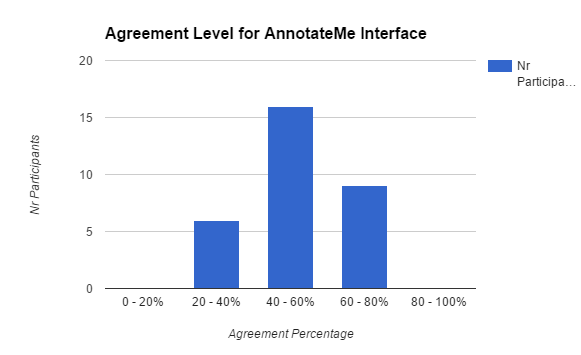
\includegraphics[width=\linewidth]{figures/experiment1/exp1-agreementlevel.PNG}
  \caption{Participants' Agreement level for the first experiment}
  \label{fig:ex1-agreementlevel}
\end{figure}
 

%freewill annotations
The setup of the first experiment was designed in a way that each individual participant performed annotations for 15 minuets constantly. They were not told upfront that they will be performing such tasks for 15 minutes, but were instructed to do the task until the experimenter told them to stop. After the estimated time elapsed they were asked whether they would like to continue do more annotations or stop and conclude the experiment. Participants were not encouraged to do any annotations after the 15 minute time trial had passed, thus the rest of annotations performed were completely voluntary and considered as free-will annotations. On average, each participant performed 22 annotation rounds during those 15 minutes. In terms of free-will annotations, one participant performed 17 annotation rounds on average. These results are used later to compare with the gamified system in order to assess the perceived engagement as a measure of time spent performing \textit{free-will annotating}. 

On the post questionnaire we asked participants to evaluate their experience with the task, the usability of the interface and perceived engagement. Figure \ref{fig:ex1-postresults} reports the results on the different questions asked on the post questionnaire. It can be concluded that the participants perceived the task to be interesting and somewhat engaging with a possibility that the participants would continue perform such task in the future. Regarding the usefulness of contextual clues, the graph indicates that users perceived the clues on average as useful when disambiguating a named entity. In addition to that, we report also on the perceived frustration while performing the task. Figure \ref{fig:ex1-frustration} indicates that the participants were seldom frustrated during the annotation process with some of the participants reporting to having been frustrated about half of the time. This can be an outcome of the participants being not familiar with the entities since they did not have the freedom of choosing a specific category or genre during the first experiment. 

%post questionnaire results 
\begin{figure}[]
  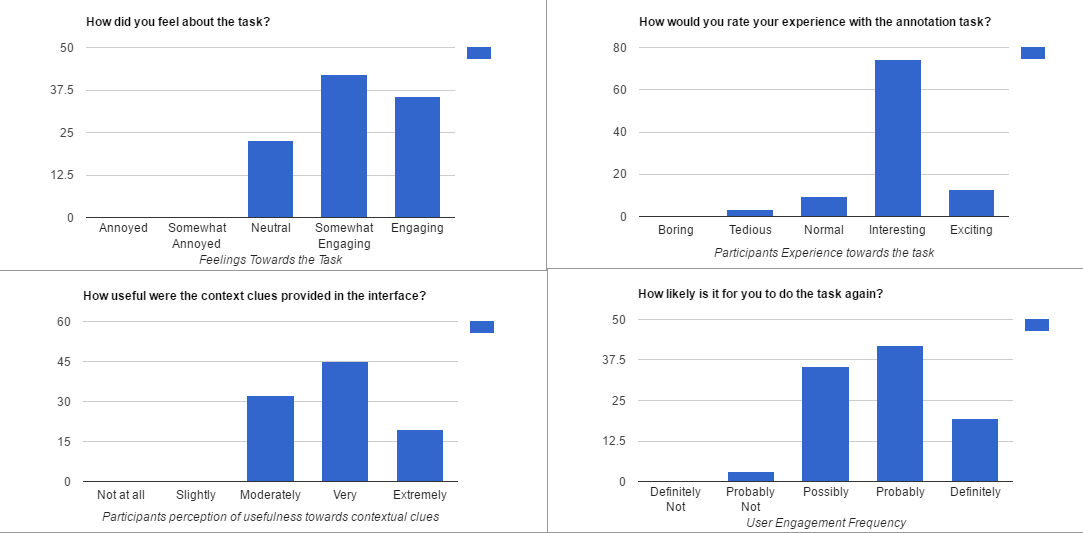
\includegraphics[width=\linewidth]{figures/experiment1/ex1-postquestionnaire.PNG}
  \caption{Experiment 1 Post Questionnaire Results}
  \label{fig:ex1-postresults}
\end{figure}

\begin{figure}[]
  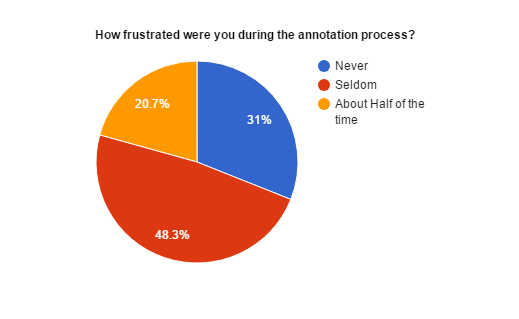
\includegraphics[width=\linewidth]{figures/experiment1/ex1-frustration.PNG}
  \caption{Reported level of frustration experienced during the annotation process}
  \label{fig:ex1-frustration}
\end{figure}

%Short contextual clues are preferred towards complete sentences or paragraphs and they provide sufficient information to make correct annotation decisions!

%What the chapter said - conclude the chapter
\chapter{Fastype - Gamification of \ac{ned}}
\label{chap:gamechapter}
%Intro to the chapter
In the previous chapter we presented the named entity disambiguation framework which has been implemented as the initial part of the work conducted for this research study. The results after conducting a user study by using a plain interface which we called the AnnotateMe Interface indicate that non-expert users are able to perform qualitative annotations with the help of short contextual clues and an intuitive user interface. However, results also indicated seldom levels of frustration during the experiment in addition to a slight percentage feeling indifferent/neutral towards being engaged or positively motivated in performing the task. For the long-term run, we assume that the plain interface lacks elements of engagement and does not have any associated intrinsic motivation that will bring users back to perform annotations. We hypothesize that by gamifying the system appropriately, it will be possible to increase user engagement with the annotation task and thus increase intrinsic motivation for participation.\if If we manage to intrinsically motivate the users with the game design elements integrated in the annotation task than we are able to claim that it is possible to retain users for a long period of time which makes it possible to generate large-scale annotation corpora.\fi In this chapter we provide an outline of related gamified systems in the field of semantic web and natural language processing (\ac{nlp}) and background information on specific game design and theoretical models on which we base or work. The chapter proceeds by explaining the methodology used from the game implementation, preparation for the second user study and the metrics and assessment techniques used to analyze the data and report on the results. 

\section{Background}
\label{game:background}
%Pontsification - not enough
Gamification is not about taking an already existing system and decorating it with points, levels and leaderboards. This methodology of gamifying a system is referred to as "Pontsification" where the game design exclusively relies on points, badges and leaderboards \cite{47}. Zichermann et al \cite{48} argues that the technique of "Pointsification" comes as a result of lacking creativity and represents a poor approach to gamification. In order to create a gamified system that truly engages users and affects their needs for satisfaction, a game designer should put more work and effort than just throwing points, badges and leaderboards into the system hoping for users to feel engaged. 

The \ac{sdt} and its sub-theory \ac{cet} have been explained in Section \ref{thb:gamedesign} and serve as the foundations on which we base our gamification model and aim to reach the goal of positively affecting users needs for satisfaction, which (accrding to \ac{sdt} and \ac{cet}) results in increased intrinsic motivation. Before we proceed with state-of-the-art gameified systems, it is important to understand some key concepts that compose a well designed game. In gamification, the most frequently used framework is the MDA Framework \cite{47}. It is one of the most leveraged frameworks of game design and it is an abbreviation of the terms: Mechanics, Dynamics and Aesthetics.
% MDA framework
\begin{itemize}
    \item \textbf{Mechanics} compose the functioning of the game. Mechanics allow a designer to have complete control over the levels of the game, giving the ability to guide the players' actions
    \item \textbf{Dynamics} are the interactions of a player with the game mechanics. They determine the action of the player in response to the mechanics of the system
    \item \textbf{Aesthetics} of the game are the elements that define how the player is feeling during his/her interaction with the game
\end{itemize}
 
By carefully studying and exploring these models and frameworks when working on the game design, it will be genuinely possible to transform a system from being monotone and tedious to something that is interactive and fun to do. 

% Stats on game play 
A well designed game or gamified system can be used to gather large-scale amount of data and information. This data can potentially open doors to improving advanced systems such as search engines or helping scientific researchers find solutions to complex protein structures by using the computing power of the people (See Foldit \cite{53}). Entertainment Software Association did a survey to find out what are the characteristics of an average gamer and how much time gamers spent playing video games, and the following statistics were reported \cite{49}:
\begin{itemize}
    \item An approximation of 5 million Americans will spend 40 or more hours a week playing games, which is the equivalent of a full time job
    \item 60\% of Americans are gamers
    \item During 2013 the gaming industry was worth 22 billion dollars, with 16 billion spent on game content only 
    \item Females account for 50\% of gameplay and purchases
    \item The average gamer is 36 years old
\end{itemize}


\newpage
\begin{figure}[]
  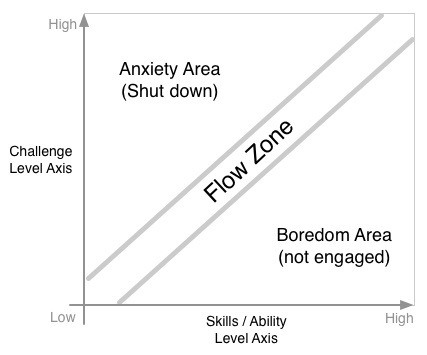
\includegraphics[width=.8\linewidth]{figures/experiment2/flowzone.png}
  \caption{The flow zone of a gameplay \cite{49}}
  \label{fig:flowzone}
\end{figure}
%Flow zone
A very important aspect in game design is the ability of maintaining the so called "Flow Zone" during the gameplay. The success of a game is achieved if the player is constantly kept within the flow-zone which is placed between anxiety and boredom \cite{49}. As illustrated in Figure \ref{fig:flowzone}, achieving flow or being in the "flow-zone" indicates the players' state of not being too overwhelmed with challenges but also avoiding the state of being bored because the game continues to offer easy challenges to the player. Zichermann et al. \cite{48} argues that a game designer must create a careful interplay of the system with the player by relentlessly testing their interactions until the point in which the player is between anxiety and boredom. This rule is applied from the first interaction of the player with the system which brings us to another quite important point in game design: Onboarding. 

%importance of onboarding 
According to Zichermann et al. \cite{48}, statistics from the casual games market show that the first minutes a player interacts with the game are the most important. This is because during the first minutes the player makes a decision whether he/she likes the game and will continue to play or not. Therefore, onboarding plays a crucial role to the overall success of the game. Onboarding is defined by Zichermann as the act of bringing novice players into the system. The responsibility of this part of the game is to carefully reveal the complexity of the system to the player without overwhelming him with too much information. In short, the goal of onboarding is to train and engage players but not overwhelm them.

%importance of challegne and other aspects (the bulletlist on the last th.b. page in the notebook about gamification).
Finally, some aspects which contribute to the idea of keeping the player engaged and motivated during gameplay need to be pointed out before we proceed with the next sections. According to Siemens et al. \cite{49}, a player expects the following elements from the game:
\begin{itemize}
    \item Focused goals
    \item Challenging tasks
    \item Clear and compelling standards
    \item Protection from failure
    \item Affirmation
    \item Novelty
    \item Freedom of choice
    \item Authenticity
    \item Affiliation with others
\end{itemize}
For our Fastype Game we have tried to employ most of these important aspects of game design in order to achieve high levels of engagement and intrinsically motivate players to interact with the game without any other form of incentive except the incentive of being entertained.
\section{Related Work}
\label{game:relate-work}
The emergence of platforms which contribute to the concept of having a group of individuals commit to creating a collective solution that is far more powerful and robust than individual ones has drawn the curiosity of many industries during the recent years. This concept is referred to as Collaborative Resource Creation (\ac{crc}) and is being utilized by systems that inherently want to use the creative and powerful nature of human thinking as a source of solving different computationally complex problems. Wikipedia can be considered as the best known example of collaborative resource creation. Furthermore, Open Mind Common Sense (\ac{omcs}) movement demonstrated that Web collaboration can be used as a tool to create \ac{ai} resource. Games can also be considered as \ac{crc} system. \cite{44, 43}

Wikipedia and \ac{omcs}, as non-gamified systems, rely on peoples' altruism and interest on science in order to commit to contributing. Whereas games provide the feeling of being entertained, and as a result the solely rely on user intrinsic motivations. Von Ahn et al. \cite{vonahn} argues that the desire to be entertained is a much more powerful incentive than any other incentive technique. It has been estimated that more than 9 million person-hours are spent by people playing games on the WEB. Dedicating a small amount of those playing hours to contribute to the solution of complex computational problems will result in tremendous benefits. This is the reason why Games With A Purpose (\ac{gwap}) are being frequently used in many domains such as \ac{nlp} and Semantic Web. Gamifying a system for the purpose of solving or facilitating computationally complex problems can be unquestionably powerful when doing it right. An excellent successful example of such a system is Foldit \cite{53}. 

Games are also used in education, generally as serious games and as digital game-based learning. In this field, gamification is defined as the use of game-based mechanics, aesthetics and game thinking to engage people, motivate action, promote learning and solve problems \cite{47}. Seaborn et al. \cite{47} argues that gamification has been used as a means of collaborative resource creation by numerous studies which take advantage of the alleged motivational benefits that game design can provide. However, almost all of these attempts of \ac{gwap} lack empirical research and standard of practice for design and implementation \cite{47}. In our work, we have attempted to analyze and understand empirical theories such as \ac{sdt} and \ac{cet} which guided the implementation of a \ac{gwap} for named entity disambiguation which resulted in a collaborative resource creation system generating training data for supervised \ac{wsd} and \ac{ned} algorithms respectively. 

Seaborn et al. \cite{47} also reported statistics on the usage of gamificaion across domains ranging from sustainability to health and wellness to education. The findings reported by the study indicate that the fields in which gamification has been mostly applied are Education (35\%), health and wellness (13\%), online communities and social works (13\%), crowdsourcing (13\%) and sustainability (10\%). They also report that a large majority of applied gamification research did not mention or address any theoretical foundations \cite{47}.

Gamification has been used as a mechanism to solve various \ac{nlp} and semantic web problems. Kaboom \cite{41} is a gamified \ac{wsd} system that can be classified as a 2D video game in the style of Fruit Ninja game. In this game, players are asked to destroy pictures that are not related to a specific term or concept shown to them beforehand. This approach aims to disambiguate word senses by using pictures as sense descriptors. The pictures that are kept at the end of a game round are considered to be related senses for the ambiguous word. Senses for each ambiguous word in the game were collected manually by expert annotators. Unlike them, we use our implemented microservice framework for generating game data instead of manually creating them, which gives us a headstart in focusing more on the game design aspect. Similar to our findings, Jurgens et al. \cite{41} also reported that game-based annotation systems reduce the cost of producing equivalent resources via crowdsourcing at least by 73\% while providing similar quality of annotations. Using Kaboom \cite{41}, they also reached a 16.3\% improvement in accuracy over state-of-art \ac{wsd}.

Phrase Detective \cite{44} is another gamified system that was developed to annotate corpora for anaphora resolution. Anaphora resolution is a semantic task used for recognizing that a pronoun like "it" and the definite nominal "the town" refers to some entity as a proper name \cite{44}. They argue that a successful \ac{gwap} should make use of all available incentives, namely, personal, social and financial. The game interface should be easy to use, intuitive to learn and designed to engage ones intended player demographic. Furthermore, they emphasize validation as a strong and effective method for quality control. By collecting multiple judgments for each expression, the gamified system can provide quality control and collect useful linguistic data. We employed some of the proposed methods by Phrase Detective as they proved to be appropriate for the design of our game, Fastype. 

To help with the creation of named entities, Green et al. \cite{50} developed the \textit{Entity Discovery} game where players are asked to annotate sentences by marking all named entities found in it. The game is played in pairs and when real players are not online to be paired with, a BOT is used instead. In order to validate the recognized entities by the first game, they developed a second game called \textit{Name that Entity}. The second game was designed as a multiple choice game were the paired players had to choose the type of the recognized entity. The game accepts a specific type for the recognized entity only if the paired players agree upon the type. \cite{50} 
In contrast, we automated the entity recognition task using our framework and for the validation task we use multiple judgments and rely on agreement levels between players which proved to be very effective and assured high quality of annotations. 

Several research studies investigated individual game elements and their impact on intrinsic motivation and performance \cite{43,45,46}. Badges, leaderboards and performance graphs, as reported by Sailer et al. \cite{45}, positively affected competence and need satisfaction. The same game elements also seemed to contribute to an increase in perceived meaningfulness as it is known that these game elements can create meaning at the game level \cite{45}. Unsurprisingly, Mekler et al. \cite{46} found that pontsification (points, levels and laderboads) functioned as extrinsic incentives effective for promoting performance quantity. They used an image annotation game to determine the effect of these three most commonly employed game elements on needs satisfaction, intrinsic motivation and performance. Using a two-fold experimental study, the game element group performed better in terms of annotation quantity, whereas the quality remained the same. Against their expectations, the different conditions (groups) did not differ in terms of intrinsic motivation or competence as a factor that impacts needs satisfaction. Possible factors that contributed to this outcome is that the game did not provide enough challenge to the players, the feedback was insufficient in determining player performance and the game lacks visual and aural presentation of game elements and feedback to the player. We try to overcome these obstacles by designing a game that keeps the user constantly engaged by increasing challenge as the player progresses, provide visually appealing feedback, empowered social elements, encouraging self-empowering through performance graphs etc. 
\section{Game Design}
\label{game:design}
Games With A Purpose (\ac{gwap}) are implemented in many fields and come in various forms. With regards to their overall game design, they tend to be graphically rich, provide simple interactions and give the player an experience of progression by scoring points, leveling players up and recognizing their effort. Additionally, the design of the game should reinforce quality measures and control the behaviour of players. Encouraging players to concentrate on the task and discourage them from malicious behaviour is crucial for quality control \cite{42}. The goal of our research study was to develop a \ac{gwap} that would serve as a tool for validating the named entity disambiguation task. The validating process should be performed at the highest quality level possible and still maintain player engagement by positively affecting their intrinsic motivation: experiencing feelings of competence, autonomy and relatedness while playing. The following subsection explore the different game elements and the corresponding game design principles used in Fastype that make this game enjoyable, fun to play and motivate players to come back and play. This results in generating large-scale annotation data for our named entity disambiguation task without players noticing what the underlying purpose of the game is.

\subsection{Onboarding}
%Onboarding 
The first impression you get when meeting somebody for the first time is usually a strong indicator that determines whether you will like the company of this new person or not. Similarly, the first impression or the first minutes of interacting with a game are the most important because a player will make a decision whether he or she will continue exploring the game. According to Zichermann et al. \cite{48}, the onboarding process is critical to a successful game. A good onboarding process leaves no other options to the player but to win. It is crucial that in this stage the player will be offered with an action at which he will not be able to fail. After having completed the initial action/task, the player should be rewarded for successfully completing it. \cite{48, 43, 48}

During the implementation of Fastype, special attention was put in designing the onboarding phase as effective as possible. Fastype has been designed as a typing game where players have to type on their keyboard as fast as possible to reach high scores and improve their typing skills. Additionally, the game requires the user to focus and memorize what they type in their keyboard and also answer quiz-like questions to get additional points, reach new levels and complete various categories. All these concepts have to be carefully revealed to the player during the onboarding stage. According to Zichermann et al. \cite{48}, the onboarding process should accomplish the following things: 
\begin{itemize}
    \item Slowly reveal the complexity of the system
    \item Positively reinforce players
    \item Avoid any action that leads to failure
    \item The game should learn something about players in order to personalize the game if necessary 
    \item All the points mentioned above have to be done within the first few minutes of the player interacting with our game
\end{itemize}

Except the points listed above, we also wanted the onboarding process to be slightly intriguing and mysterious in order to tease the player's curiosity. When entering the game site, the players are presented with a screen which requires them to know a \textit{ game secret} (See Figure \ref{fig:game-startscreen}). Having a secret comination to enter the game might potentially affect feelings of relatedness as the player will experience feelings of being part of a secret game club which allows entrance only to players who are aware of the game secret. However, the game provides a way of discovering the game secret. The only way of acquiring it and being granted with access to the game is by following a trial procedure. This trial procedure represents the onboarding process for our game. 

\begin{figure}[h]
  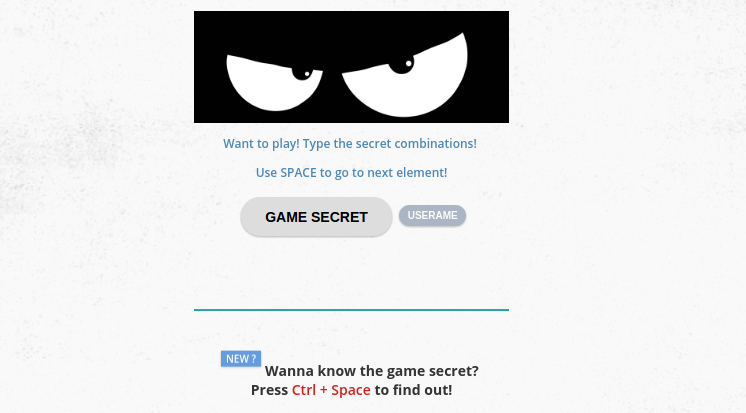
\includegraphics[width=\linewidth]{figures/experiment2/startscreen-game.png}
  \caption{The game start screen presented to player when entering the game for the first time}
  \label{fig:game-startscreen}
\end{figure}


The onboarding process starts by asking players to type the words that appear in the screen as small boxes. Points are awarded to the player regardless of their typing speed (rewarding and recognizing the players' effort). After the player is familiarized with the way the game works (typing fast while paying attention to the words that appear in the screen), the game continues by introducing a new challenge: a puzzle combined with typing skills. The puzzle consists of several hidden characters that the player has to reveal by typing the words appearing in the screen. The faster the typing the faster the revealing of characters. After the player has revealed all the characters on the puzzle, he is presented with a quiz where the \textit{question} is the revealed word (i.e. the named entity) and the options are the candidate entities extracted from \ac{kb}. Contextual clues are provided on top of the screen as sticky notes which help the player to make a correct decision. The quiz is a \textit{masked} version of the named entity disambiguation process used in the first experiment. The player proceeds by selecting a candidate option which is rewarded with 10 game points. Please note that if the player selects the wrong option, the system will not proceed until the right option is selected. As a reward for choosing the correct answer, the player finally reaches the end of the trial process where the game secret is finally revealed. Additionally, the player has to register himself with authentication credentials which together with the game secret are used as a secret combination for granting access to the game. Figures \ref{fig:onboarding}(a) to  \ref{fig:onboarding}(f) illustrate the complete onboarding process of Fastype. 

\begin{figure}[]
  \centering
  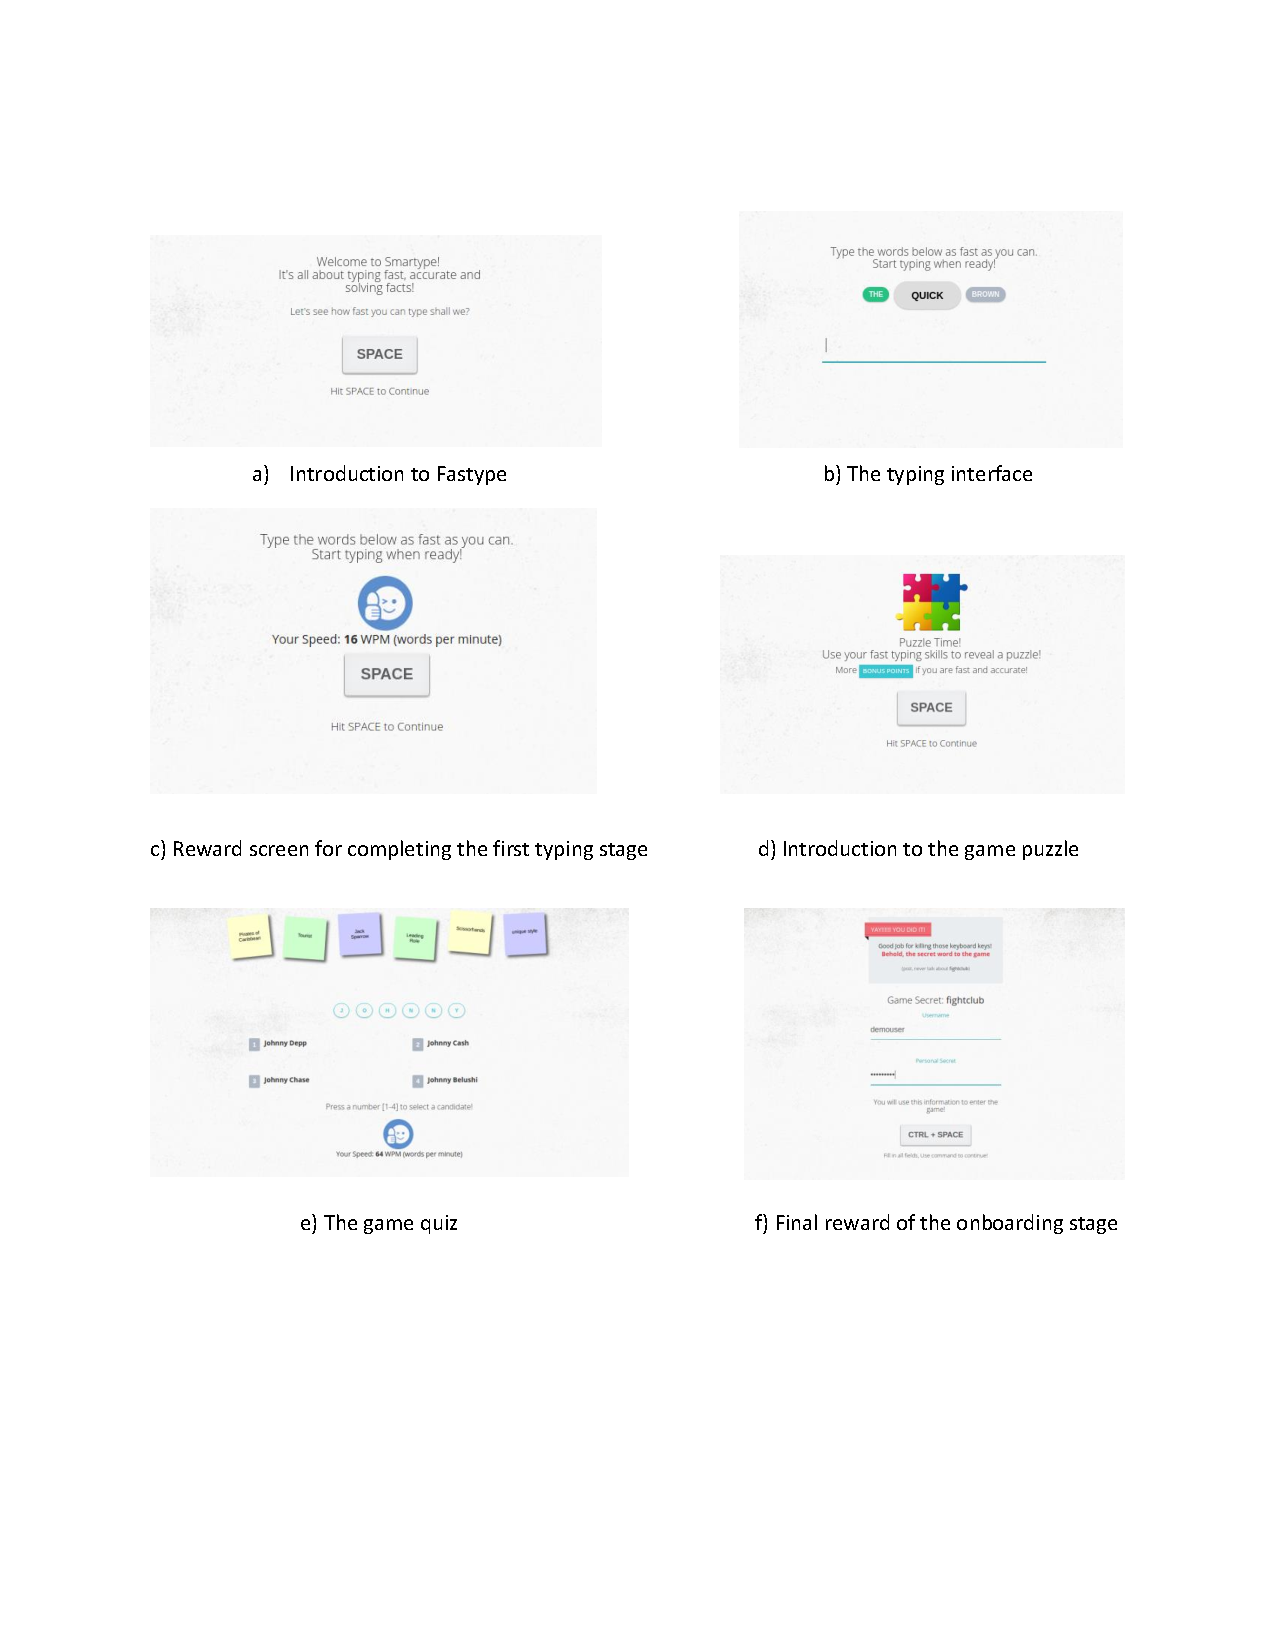
\includegraphics[page=1,width=\textwidth]{figures/experiment2/oboarding.pdf}
  \caption{The onboarding stage of Fastype}
  \label{fig:onboarding}
\end{figure}
\subsection{Task Design}
After exploring and analyzing many gamified systems and the effect of various game elements towards user engagement and motivation, Sailer et al. \cite{45} argues that gamification is not effective per se, but specific game design elements have specific psychological effects. Thus, it is important that gamification is not done just by incorporating a scoring system with some levels to advance and a leaderboard to see your progress. It takes more than that to design a game that attracts and retains a player base. 

Chamberlain et al. \cite{43} emphasizes that it is the design of the individual tasks in a gameplay that determine how successful the player can contribute data whilst playing. Furthermore, Sailer et al. \cite{45} communicates the importance of game elements being recognized by the player in the gamified environment. Delivering the treatment to the player or to a participant in the game is not enough unless the designer of the game makes sure that the treatment is also received by them. Failing to design treatments or game elements that are genuinely recognized by the players, results in loss of statistical power and risk to underestimate their effectiveness \cite{45}. In order to adhere to the aforementioned design constraints, significant work effort was placed in designing a task that contributes to generating annotation data of good quality. 


A game-round starts by the player selecting a specific category to play or letting the game choose a category in a random fashion for the player. Everything in the game is designed in a way that the player only has to use the keyboard for completing almost every action. The player is then presented with the typing screen where a combination of hidden characters have to be revealed by typing as fast as possible. Figure \ref{fig:game-typingscreen} illustrates the typing screen. A speed radar is placed right underneath the typing text box which displays the current speed of typing measured as the amount of words typed per minute while the player is revealing the hidden characters. This element can be considered a strong motivator to keep the player focused on typing fast. After having revealed the word, the upcoming challenges/questions all revolve around the text that has been typed during the typing phase. The players are already familiar with this concept since a similar task was already performed during the onboarding phase. Bonus questions are immediately presented to the user after completing the revealing stage (we talk more about the importance of bonus questions towards the overall design in a later subsection). The content of the bonus questions is created by using the text that was typed in the previous stage. Similarly, the most important part of the game that contributes to the original task of disambiguating entities is the quiz stage of the game. The quiz interface provides contextual clues extracted from our original framework and lists all the potentially candidates (quiz options) from which the player has to choose. 

\begin{figure}[]
  \centering
  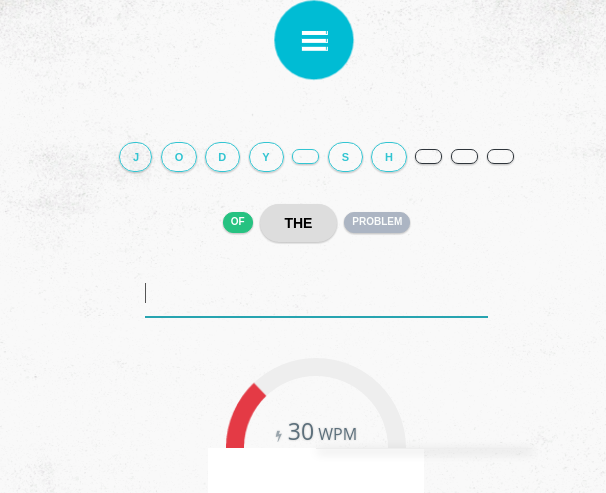
\includegraphics[width=.6\linewidth]{figures/experiment2/gameplay1.png}
  \caption{The typing screen and the speedometer calculating the typing speed of the player}
  \label{fig:game-typingscreen}
\end{figure}

We strongly emphasize the fact that all the game elements presented so far are focused and contribute to the ultimate goal, which is annotating the entity with the right candidate. The text which the player types during the typing stage, the content of the bonus questions and the contextual clues all represent carefully carved information that contribute in helping the player choose the right candidate. We make sure that the typing text\footnote{During the fast-typing stage, players are presented with different words that appear on the screen one after another. These words are part of a complete paragraph that is taken from the document where the target entity is part of.} as a game element is recognized and takes the attention of the player because if players are able to remember the text they typed, they can get points from correctly answering the bonus questions and also be confident on the candidate option they select. An example of a bonus question is presented in Figure \ref{fig:game-bonusqeustion} while the quiz interface of the game is illustrated in Figure \ref{fig:game-quiz}. 

\begin{figure}[]
    \centering
    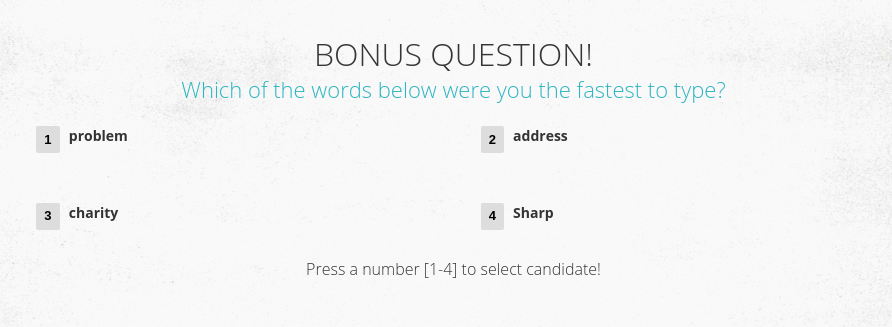
\includegraphics[width=.8\linewidth]{figures/experiment2/bonusquestion.png}
    \caption{An example of a bonus question}
    \label{fig:game-bonusqeustion}
\end{figure}

\begin{figure}[]
    \centering
    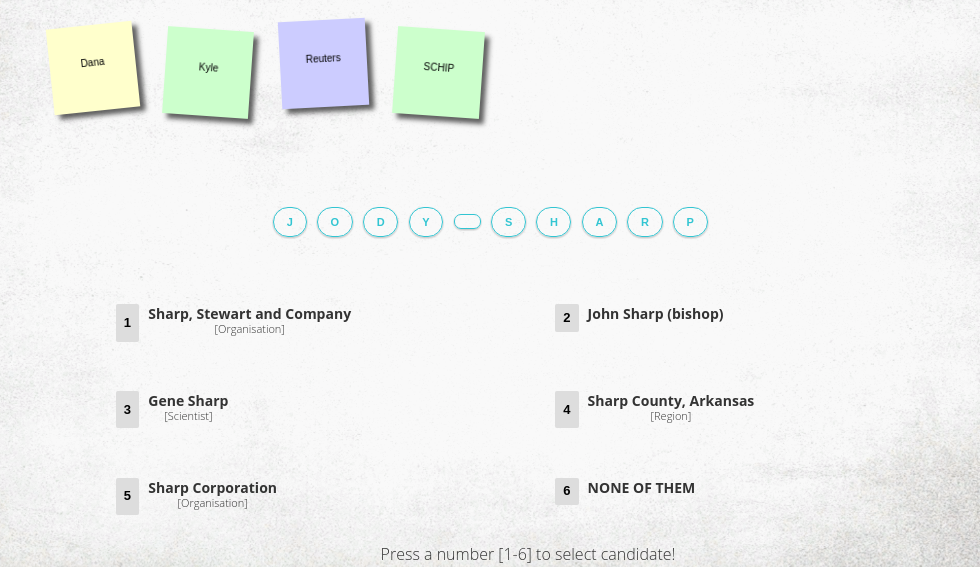
\includegraphics[width=.6\linewidth]{figures/experiment2/game-quiz.png}
    \caption{Interface of the game quiz - a gamified version for the named entity disambiguation task}
    \label{fig:game-quiz}
\end{figure}

%Skillset required/improved in the game
Schell \cite{51} (page 214) emphasizes the importance of the skill and chance mechanisms in games. A good game should balance between skill and chance during the gameplay. We believe that we have reached a satisfactory balance between these two factors by equalizing the factor of chance and skill required. The factor of luck is represented by bonus questions which are extracted from the typing text and are genuinely hard to answer since a memorization of everything typed is required. On the other hand, the factor of skills is represented by the quiz element of the gameplay. Correctly answering the quiz requires certain skill-sets from the player in order to maximize their profit point-wise. Except requiring skills from the players, the game should also contribute in allowing the players to master and perfection these skills. In general, by playing Fastype, a player will improve the following skills:

\begin{itemize}
    \item Typing skills
    \item Concentration in time pressure 
    \item Memory training and pattern recognition
    \item Knowledge in different categories (politics, music, entertainment, health etc)
\end{itemize}

Improving these skills is one of the goals that players will attempt to achieve. After having observed the players during their gamplay when conducting the second experiment we are aware that the goals of the game are concrete, achievable and rewarding at the same time. Having all these three elements characterizing the goals of the game is crucial to keeping players engaged and motivated \cite{51}. 

Reviewed literature suggests a number of criteria for evaluating enjoyment during gameplay. Some of the criteria which apply to task design and which also relate with SDT in terms of their importance towards increasing intrinsic motivation include: Feedback and Immersion \cite{41}. Constant feedback is given to the player for every performed action when interacting with Fastype. Immersion in our case refers to a short and arcade style of the gameplay which make the player experience a deep and yet effortless involvement in the game \cite{41}. A game round in Fastype lasts 4-5 minutes on average with the player being exposed to different challenging tasks. This results in an effortless and deep involvement in the game for a short period of time. Additionally, the game elements and the feedback provided during the gameplay have been enriched with sounds, visuals and animations which according to Mekler et al. \cite{46} can positively affect competence, needs satisfaction and subsequently increase intrinsic motivation.

%performance graphs, levels, leaderboards, points 
Game elements such as performance graphs, levels, points and leaderboards are provided in the game in order to give the players the feeling of progression and advancement. With these game elements we also reinforce the competitive nature of players to compete with others but also work hard on breaking their personal best scores. This results in encouraging players to get better each time they enter the game (mastery of skills). Figure \ref{fig:game-profile} illustrates the profile of the player where a performance history of the typing speed is provided in addition to level information, challenge status and betting ratio (a balance between the bets lost and won).

\begin{figure}[]
    \centering
    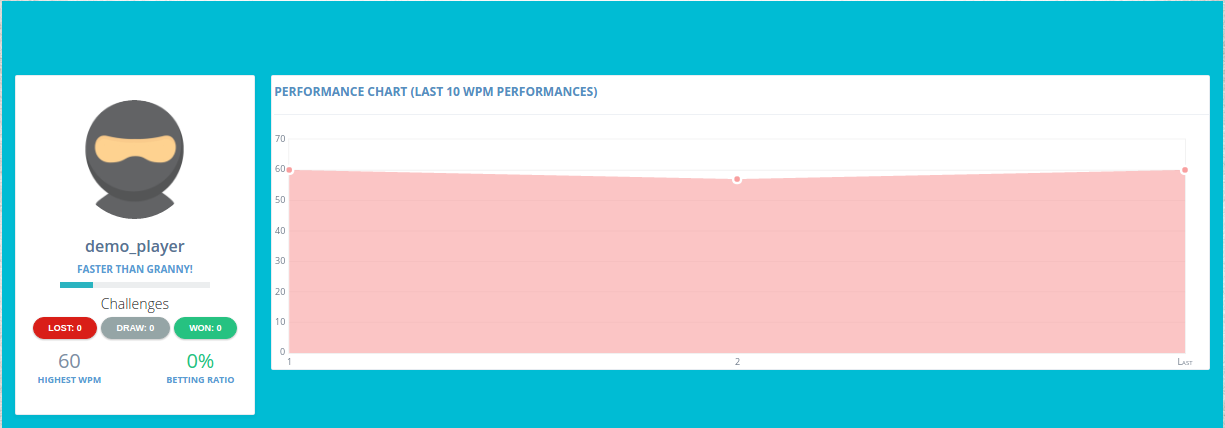
\includegraphics[width=\linewidth]{figures/experiment2/profile.png}
    \caption{Player profile screen}
    \label{fig:game-profile}
\end{figure}

The final element that requires our attention is the concept of game-flow. It was explained in the background section of this chapter that game-flow is the concept of keeping the player constantly engaged while not overwhelming him with problems that are too complex to overcome or too easy that the player gets bored quickly. Our idea of keeping the complexity of the game in the same level as the player's progression and skill improvement in the game is by increasing the total number of words that players have to type within a game-round. The complexity is controlled by the level mechanism of the game. When players progress and reach new levels, they are faced with longer and more complex paragraphs to type. However, one can argue that this is not the best and most optimal way of maintaining game complexity and player's flow zone. Being limited in the amount of resources available to be spent in designing and implementing all the game elements, the proposed idea of defining and maintaining game complexity was the only achievable concept within these constraints. However, ideas to improve the existing design of game complexity will be addressed in the discussion section and as such will be accounted for future work. 

\subsection{Freedom of choice}
%Autonomy - Freedom of choice - categories 
%training phase
During the first experiment where the non-gamified interface was used to perform annotations, many participants addressed the fact of not having control over the genre of the entities presented to them. Since the selection of the entities to be resolved was done in a random fashion, one of the participants was constantly getting entities that fell into the Arts category. As a consequence, the participant was feeling very insecure during the task because of being unfamiliar with most of the concepts being presented to him. We would like to stress out the importance of freedom of choice in this aspect. Being able to freely decide what category to play in, is an important factor for reinforcing autonomy and competence. As a result, the game gives the player the freedom of choice by providing several game categories to choose from. For players who like the aspect of surprise and chance, the game can make a random choice for the player if instructed to do so. 

Furthermore, the game provides a training phase for players who feel unprepared to take the actual task where the performance is recorded. According to Chamberlain et al. \cite{43} GWAP usually begin with a training phase so that players are able to practice their skills and also show that they have understood the instructions before they do the real task. However, in our case the onboarding stage takes care of explaining the complexity and instructions for performing actions in the game while the training phase allows the user to practice their typing skills. The training phase was also designed for the purpose of getting familiar with a new keyboard since the participants played the game from the experimenters laptop and therefore it was necessary to have a training phase. The game acknowledges the player for the existence of a training possibility in the game by pushing notification on the screen.
\subsection{Game challenges}
%Challenges 
%Punishmet
Von Ahn in his pioneering work \cite{vonahn} focuses on one type of incentive to motivate players: enjoyment. He emphasized that the main mechanism to make players enjoy a GWAP is by providing them with a challenge. Usually in many gamified systems, challenges are achieved through mechanisms such as requiring a timed response, keeping scores which ensure competition among players, having players with similar level of skill compete against each other and so on. \cite{44} 

The design of Fastype strongly reinforces the competitive nature of players by providing challenges which allow players to compete with each other. During each game round, the system keeps track of the player's typing speed, and shows potential challenges based on their WPM (Words Per Minute) accordingly. To assure fair play, the system makes sure that the player is presented with challengers that have roughly the same level of skill. The challenge screen is presented to the player after she has completed the quiz. Figure \ref{fig:game-challenge-screen} shows the exact challenge screen which is used by players to send challenge requests to other players in the game. As seen in the figure, players can choose a number of points between 1 and 10 to challenge the other players. These points represent the reward or punishment mechanism of the challenge. To assure fair play of the game, players who are challenged will type the exact same words as the challengee, therefore an accurate measure of their skill is guaranteed. Finally, having a challenging game where each challenge matches the players skill level contributes to the feeling of enjoyment during gameplay \cite{43}.

\begin{figure}[]
    \centering
    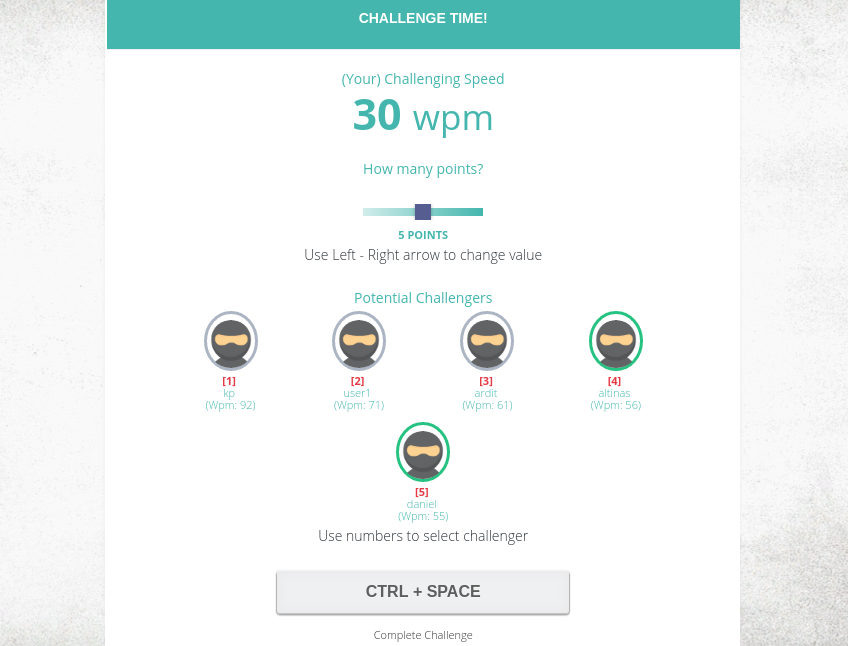
\includegraphics[width=.8\linewidth]{figures/experiment2/challenge-time.png}
    \caption{Fastype Challenge Screen}
    \label{fig:game-challenge-screen}
\end{figure}

An additional note that requires attention is the mechanism of punishment in a game. Schell \cite{51} (page 225) addresses the importance of punishment mechanisms in games and if balanced appropriately, they will give more meaning to everything in the game. Punishment mechanisms increase the value of certain game elements such as points. In Fastype, challenges and the betting mechanisms provide a way of punishment for players. In case of failure, their accumulated game points will be taken away, subsequently dragging the player down in lower levels in addition to increasing the failure percentage in their profile. Please note that the players have always the option of skipping challenges or bets on their answers. As a consequence of avoiding challenges and bets in the gameplay, the player will experience a slow progression and less dramatic gameplay as compared to other players who take risks by betting and challenging other players.
\subsection{Bonus Questions} 
%lens of chance
%the element of surprise, random nature (never know what to expect), have to rembmer all what was written and how it was written, a skill which is hard to master but interesting and misterious and with the help of chance it is sometimes easy achieved
The bonus questions represent the element of chance and surprise in our gameplay. The random nature of the bonus questions give the game a unique flavor of mystery and surprise since the player never knows what to expect from the bonus questions and therefore it encourages players to work on remembering what and how she was typing. Some bonus questions ask about the total number of words typed, the fastest word typed, the number of times a player failed to type a word correctly, the number of times a specific word occurred etc. The bonus question play an important role in the overall playfulness and feelings of enjoyment during gameplay. 
\subsection{Betting System - a measure for quality control}
Many of the existing gamified systems point out the importance of quality control in \ac{gwap}. Von Ahn et al. \cite{44} suggests two mechanisms for ensuring correctness of data: player testing \footnote{Player testing is evaluating the players output by occasionally matching it against gold standards or already annotated data} and repetition or redundancy of data. In our game design we have employed two mechanisms for ensuring that the quality of annotations performed through the game is maintained. 
The first assessment methodology is accumulating multiple individual answers for a specific entity before deciding whether that answer is correct or not. This corresponds to the redundancy of data for quality control suggested by \cite{44}. The second assessment methodology is using the betting system incorporated into the game. If we look at the betting element in the game from the eyes of a game designer, this element represents the lens of triangularity proposed by Schell \cite{51} (page 212). The lens of triangularity gives a player the choice to play safe for small rewards or take a risk and win big rewards. Triangularity gives an interesting and exciting flavour to our game. On the other hand, if we look at this game element from the eyes of a linguistic expert who demands from the game the generation of trustful and qualitative annotations, than this element represents a measure for assessing the confidence of a player towards the his choice of candidate. Figure \ref{fig:game-bet} illustrates the betting screen shown to the player immediately after having completed the quiz.

\begin{figure}[]
    \centering
    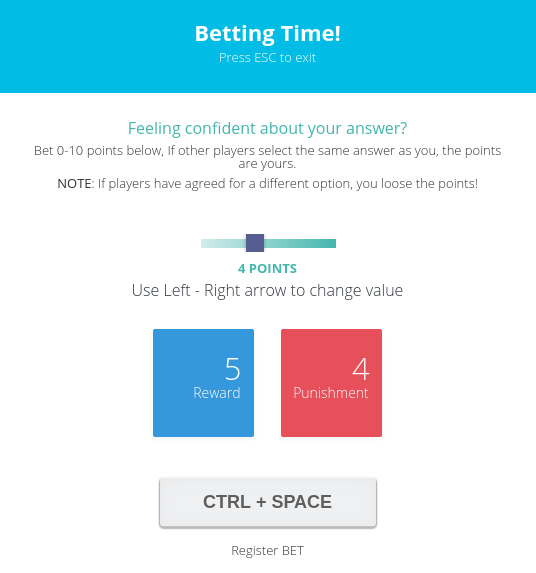
\includegraphics[width=.8\linewidth]{figures/experiment2/game-bet2.png}
    \caption{Betting Mechanism as a quality control and representative of triangularity for Fastype}
    \label{fig:game-bet}
\end{figure}

As we can see from Figure \ref{fig:game-bet}, the player has the choice of deciding the amount of points he wants to bet on the selected answer. The bigger the number of points used in the bet the higher the risk of loosing or wining them. Players are instructed to think if other players who might potentially encounter the same quiz will also choose the exact same answer as they did. In that case, if they are confident about the given answer, then the players are encouraged to place high bets rather than playing it safe. However, the choice remains completely in the hands of the player. Our betting mechanism works in the way that for one individual entity, when more than 4 unique judgments agree on the same candidate, than this entity is considered to be resolved. All the players whos' selected candidate is the same as the correct candidate (meaning their answer falls within the absolute majority) will be rewarded with the amount of points they bet for the particular entity. Similarly, all the players whos' answer was not the one selected by the majority are punished by subtracting the amount of points they bet from their overall accumulated points in the game. In terms of annotation quality, candidates with higher betting scores represent higher levels of confidence which means we can be sure that the selected candidate is undoubtedly the correct representative for the target entity.
\subsection{Social Interaction \& Engagement Loop}
%SHoutouts, challanging, desire to compete (being the first in the board) each other as relatedness factors - increasing social interaction - Relatedness is a factor that positively affects intrinsic motivation
Significant design and implementation effort was put in making the game as much socially interactive as possible. Among the three SDT elements which have direct impact in intrinsic motivation and needs satisfaction, social interaction contributes to the feeling of relatedness with others. The main social interaction mechanism implemented in the current version of the game are challenges. The desire to compete and overcome players in the leaderboard can be seen as an element that entails social interaction within the game. 

%engagement loop
The concept of engagement loop on the other hand is a fundamental aspect that needs to be clearly defined in order to maintain player motivation. A successful designed engagement loop always leaves something incomplete or pending in the game for players to come back and play. Game designer David Perry suggests that the key to addictive game design is by creating a game that keeps the player engaged by doing three things all at the time: exercising a skill, taking risks and working out a strategy \cite{15}. Zicherman et al. \cite{48} gives substantial importance to the social engagement loop and defines the following four key aspects to be considered by game designers when thinking about engagement loops: motivating emotion, player re-engagement, social call to action and visible progress/rewards. Table \ref{tab:engagement-loop} lists the game elements of Fastype that contribute to the different aspects of social engagement loop.

% Table generated by Excel2LaTeX from sheet 'Sheet1'
\begin{table}[htbp]
  \centering
  \caption{Game elements of Fastype that contribute to the social engagement loop}
    \begin{tabular}{|c|l|}
    \toprule
    \multicolumn{2}{|c|}{Social Engagement Loop} \\
    \midrule
    \multirow{Motivating Emotion} & Excercising fast typing \\
          & Competing with others \\
          & Learning new facts  \\
          & Improving Memory skills \\
    \midrule
    \multirow{Player Renegagement} & Levels \\
          & Challenges  \\
          & Increasing WPM  \\
          & Completing Categories \\
    \midrule
    \multirow{Social call to action} & \multirow{Challenges } \\
          &  \\
    \midrule
    \multirow{Visible progress} & Leaderboard \\
          & Points  \\
          & Levels  \\
          & Challenge Win/Lose Ratio \\
    \bottomrule
    \end{tabular}%
  \label{tab:engagement-loop}%
\end{table}%
\newpage
\section{Methodology}
\label{game:methodology}
% DESCRIBE THE METHODOLOGY USED TO ANSWER THE FOLLOWING RESEACH QUESTIONS

%---- What game mechanics can be employed in the entity resolution task so that high levels of engagement are achieved while still maintaining annotation quality?
The last proposed research question posed by this study is concerned in finding out what game mechanics and design principles are best fit for our research problem in order to positively affect intrinsic motivation and achieve high levels of engagement. We are also concerned to find out whether the implemented game contributes to qualitative annotations by non-experts so that we can harvest the potential of players with different levels of expertise in annotating, age group and academic background. To be able to answer our third research question and assess the usability and performance of our implemented game, we conducted another experimental user study with the same participants who participated in the first experiment. However, a different dataset was used for the second experiment. Choosing a different dataset was important since the participants were already familiar with the two datasets used in the first study. 

%Datasets 
%--Describe the stats of the dataset, nr of entities, types etc
MSNBC first introduced by \cite{24} is the dataset used for our second user study. It contains news-wire text from MSNBC news network. The dataset was created in 2007 and contains information and facts from that period. This fact was communicated and acknowledged by the participants on the second experiment in order to avoid reference errors such as linking the entity "USA President" with the candidate "Donald Trump" instead of "George W. Bush". The complete dataset contains 20 document in total, however, we used only 12 of them in order to reduce the total number of entities to deal with. Experimenting on a reduced version of the dataset instead of the complete version does not have any implications on our results. The reason we used a reduced version of the dataset is because our game relies on multiple judgments to disambiguate an entity (4 independent judgments to be precise). Therefore, having a small pool of entities to pick from would result in more entities being resolved during our time limited user experiment. The more entities resolved during the experiment the more confident the results of our analysis. In summary, we used the documents in the following categories from the MSNBC dataset for our second experiment: Entertainment, Health, Politics, Technology, Sports and World. The gold standard for MSNBC reported 251 named entities in total with an average of 20 named entities per document.   

%recruiting participants
%--Describe the experiment (setup, duration)
%-- we used the same participants as in the last experiment 
%-- not all showed up because of sickness or not being at the campus at the time of experiment
Similar to the first experiment, emails and social media were used as communication sources for recruiting participants for the second experiment. Initially, we aimed to recruit the same participants who took part in the first experiment, however, since some of the participants reported to be away or sick during the time of experiment, we sent invitations to others as well. As a result, 26 participants took part in the second experiment with 24 of them participating for the second time. 

The university campus was the environment where the second experiment was conducted. Participation was scheduled in different time-slots with a maximum duration of 40 minutes assigned for each round. Stretching the session duration to 40 minutes has been done for the only reason of giving temporal space for participants who wished to play longer if necessary. During the invitation process, it was made clear to the participants that the (mandatory) duration of the experiment would be approximately 20 to 25 minutes including the pre-questionnaire, gameplay and post-questionnaire. Similar to the first experiment, we used a consent form to communicate the purpose and the voluntary nature of the experiment. In order to assure consistency of data given by participants, a pre-questionnaire gathering demographic information was also used in the second experiment in addition to questions related to frequency of playing video games. We report on the demographic data of participants and their frequency of playing video games in section \ref{game:results} whereas the questions used in the pre-questionnaire are presented in Appendix \ref{appendix2:fastype}. 

% Assessment methodologies
The completion of the pre-questionnaire was followed with an immediate transition to the gameplay. In order to be consistent with the first experiment, players were asked to perform game rounds iteratively until the experimenter instructed them to stop. 15 minutes were dedicated for performing game rounds (annotations). However, the game includes an onboarding phase which introduces the player with the game and gradually reveals the complexity without overwhelming the player with too much information at once. Therefore, the time used by each participant to complete the onboarding phase is not recorded as part of the 15 minutes of total gameplay. The reason is that no annotation is performed during the onboarding phase of the game. After the 15 minutes of gameplay, participant were told to either finish playing or continue as they desire. This methodology was used in the first experiment as well and allows us to assess the participant's engagement with the game and its fun aspect. Finally, a post-questionnaire was used to assess player engagement, motivation, usability and enjoyability of the game. We report on the results of the post-questionnaire in section \ref{game:results} and list the questions used in this questionnaire in Appendix \ref{appendix2:fastype}.

Agreement level with the majority and comparison of game annotations with the gold standard are the methodologies used for determining the quality of annotations performed by players while playing Fastype. Besides the free-will annotation metric used in the first and second experiment for assessing the level of engagement of participants with each interface, we also employed Von Ahn and Debish \cite{44} assessment metrics for evaluating a GWAP. Von Ahn proposes two assessment metrics: \textit{throughput} which represents the speed at which a particular player is annotating, and \textit{average lifetime play} which represents a measure of enjoyability \cite{44}.


% ANOVA for comparison of game and interface, differences in number of observations, does not have any impact on results when working with small samples
Additionally, in order to report confident results, it was necessary to perform ANOVA analysis between the two conditions (AnnotateME and Fastype) for different factors such as: enjoyability, level of engagement and the likeliness of participants  to use each interface for an actual task outside the experiment. We perform one way ANOVA analysis for this purpose. For the sake of reproducability of results, it is important to note that the observations used to calculate ANOVA for the two conditions were not the same. The observations from the second experiment were slightly smaller than those from the first experiment. However, from a statistical point of view, small differences between conditions do not affect the final results when calculating one way ANOVA. Please note that ANOVA analysis were manually performed using Excel spreadsheets. Finally, to support our claims that the Fastype game was significantly more engaging and fun to play compared to the AnnotateMe interface, besides evaluating the interfaces using the aforementioned assessment metrics we sent a final assessment questionnaire to all participants who took part in both experiments. The questionnaire consisted of one question which asked about their preferred interface for performing the task of resolving named entities. This answers to the last questionnaire allow us to strengthen the claims that the game was significantly more attractive compared to the non-gamified interface. The content of the questionnaire is presented in Appendix \ref{appendix2:fastype}.  

% Likely sources of BIAS


%Hypothesis 
\paragraph{Hypothesis}
The second experiment was conducted in order to determine whether our proposed gamified system can intrinsically motivate users to perform a tedious and boring tasks such as named entity disambiguation. Another important aspect that needs to be emphasized is the quality of annotations. It is crucial for the design of the game to avoid having distracting elements that would intentionally or unintentionally degrade the quality of annotations. Keeping these important aspects in mind, we hypothesize that: 

\begin{itemize}
    \item H2.1: By employing game mechanics and design principles based on theoretical foundations, players will be intrinsically motivated to play the game
    \item H2.2: In case H2.1 is supported, we can further hypothesize that users who have used both interfaces to perform annotations will choose the game significantly more than the plain interface.
    \item H2.3: The quality of annotations performed by players will not be degraded even after implementing game elements that do not directly contribute to the annotation task.
\end{itemize}
\newpage
\section{Results}
\label{game:results}
This section reports on the results after conducting the second experiment and analyzing the effects of the different game elements towards user engagement with Fastype. We also report on the playfulness of the game, feelings of competence, autonomy and relatedness in addition to testing and comparing the quality of annotations with the first experiment. In overall, these analysis will guide the rest of this research study towards answering the last research question regarding gamification and the corresponding hypothesis.

\subsection{Participants}
%Pre questionnaires 
%difference compared to first experiment 
It was mentioned in the previous section that the recruitment of participants has been done in a consistent way with the first experiment. The participation resulted in having 27 participants in total which is 3 participants less than the first experiment. Those who did not show up for the second experiment were either not at the university campus during the whole week of experiment or were sick and could not show up. However, among those 27 participants 11.1\% (namely 3 out of 27) of them were partcicipating for the first time. This small group of participants that were not part of the first user study were not presented with questions that involved comparisons or assessment of AnnotateMe with Fastype.

The pre-questionnaire for the second experiment was designed for gathering information about players' demographic data in addition to information related to their gameplay frequency. The questions related to gameplay frequency will provide approximate insights on how often participants play video games and see if this is a potential bias on the quality of annotations and evaluation of the game. Regarding demographic data (since 89\% of participants were participating for the second time) we report similar results: the average player is a 25 years old male student who studies in a computer science related field who occasionally plays video games with an average of 8 hours played during the last month. Figure \ref{fig:game-prequestionnaire} presents two graphs which report on the gamplay frequency (left figure) and average hours played (right figure) during last month. From the results of the pre-questionnaire, it can be concluded that our participants in general can not be considered as expert gamers based on their frequency of gameplay. However, on average the participants have a mix of different gaming frequency as observed on the left graph in Figure \ref{fig:game-prequestionnaire}. Therefore we argue that the population sample used for this experiment represents the potential average player of Fastype outside the experiment. 


\begin{figure}[]
    \centering
    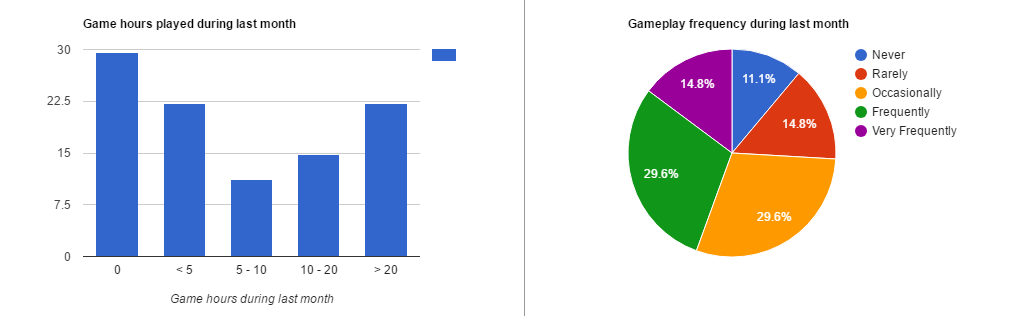
\includegraphics[width=\linewidth]{figures/experiment2/game-prequestionnaire.PNG}
    \caption{Results on participants' gameplay frequency for Experiment 2}
    \label{fig:game-prequestionnaire}
\end{figure}

\subsection{Annotation Performance}
%DBPedia autmatoc likinng accuracy - 228
All the data used in the game has been automatically generated by the framework. The only task which was manually performed by the experimenter was uploading the MSNBC documents into the framework through the admin interface. The rest was carried out automatically from recognizing the entities to generating the corresponding Dbpedia candidates. 

Regardig the number of entities available in the MSNBC dataset, our NER microservice recognized 228 entity mentions in total. Corresponding F-Measures were used to calculate the performance of the entity recognition service using MSNBC dataset and resulted with 0.77 for precision, 0.83 for recall and 0.8 for the f-score. The performance of other automatic annotators in terms of entity recognition are presented in Table \ref{tab:ex2-ner-performance}. We observe a very small improvement on the overall F-score of our framework compared to AIDA which performed best among the other automatic annotator. However, improving entity recognition performance is not the scope of this study and therefore we will not elaborate on the respective \ac{ner} performance results. 

% Table generated by Excel2LaTeX from sheet 'Sheet4'
\begin{table}[htbp]
  \centering
  \caption{NER performance on MSNBC dataset}
    \begin{tabular}{|l|c|c|c|}
    \toprule
    \textbf{-/Dataset} & \multicolumn{3}{c|}{\textbf{MSNBC Dataset}} \\
    \midrule
    \textbf{Annotator/Metric} & \multicolumn{1}{l|}{\textbf{Precision}} & \multicolumn{1}{l|}{\textbf{Recall}} & \multicolumn{1}{l|}{\textbf{F-Score}} \\
    \midrule
    \textbf{Babelfy} & 0.45  & 0.65  & 0.52 \\
    \midrule
    \textbf{Dbpedia Spotlight} & 0.58  & 0.6   & 0.57 \\
    \midrule
    \textbf{AIDA} & 0.92  & 0.71  & 0.78 \\
    \midrule
    \textbf{Dexter} & 0.49  & 0.66  & 0.39 \\
    \midrule
    \textbf{Fastype (Experiment 2)} & \textcolor[rgb]{ 1,  0,  0}{\textbf{0.77}} & \textcolor[rgb]{ 1,  0,  0}{\textbf{0.83}} & \textcolor[rgb]{ 1,  0,  0}{\textbf{0.8}} \\
    \bottomrule
    \end{tabular}%
  \label{tab:ex2-ner-performance}%
\end{table}%

%24 entities 
The performance of the automatic annotator used by our framework, namely Dbpedia Spotlight, in terms of accuracy of linking the identified entities with the correct candidate has been calculated as well. When querying Spotlight for a specific entity, a list of candidates is returned correspondingly with each candidate associated with a final score. The candidate with the highest final score is considered by Spotlight to be the correct link associated with the target entity. We run our analysis on all the 228 recognized entities and checked for each entity whether the associated candidate with the highest final score was the correct representative based on the gold standard of MSNBC provided by GERBIL \cite{40}. Among the 228 recognized entities, Spotlight linked 66.35\% of them correctly and 33.65\% incorrectly. This shows a significant improvement compared to the datasets used in the first experiment. A possible explanation for the observed improvement is the nature of the dataset. The entities recognized in MSNBC have a less ambiguous nature compared to the KORE50 and Spotlight datasets used in the first experiment. As a result the automatic annotator improved its performance. 

Before proceeding with reporting on the performances of the non-expert annotators, we report on the total number of entities resolved during the experiment. The assessment technique used for evaluating an entity based on the participants judgment is the same as for the first. The game accumulates four different judgments from independent annotators before resolving an entity with a specific candidate. Among the 228 entities recognized in total, only 24 of them were resolved while the second experiment was being conducted. Unfortunately, this is 60\% less entities resolved in the second experiment compared to the first experiment. The reason for this outome is because the average tasks/game-rounds completed during a session dropped significantly for the game. The game elements such as fast typing, bonus questions, bets and challenges are all additional tasks that take significant amount of time to complete. Besides the fact that the game elements enrich the experience, improve player engagement and increase intrinsic motivation, they did slow down the annotation process significantly more compared to AnnotateMe Interface. One might argue that drawing conclusions on such a small sample of resolved entities does not necessarily generalize to the whole population. We recognize this issue in our analysis and therefore we address it as a limitation on our results. However, the potential of the game is significantly higher compared to the plain interface used in the first experiment and we predict that the game will still perform much better in terms of user engagement and maintain annotation quality regardless of the number of annotations resolved. 

%ANOVA difference between DBpedia anntator and human - in accuracy (report the f-scores)
Among the 26 resolved entities 95\% were correctly linked with a Dbpedia candidate whereas 5\% were incorrectly linked when compared to the gold standard. Table \ref{tab:ex2-annotation-performance} shows the performance of the game and Dbpedia Spotlight on all 26 resolved entities in terms of precision, recall and f-score measures. The game which used non-expert annotators exhibits a slight improvement compared to the automatic annotator. However, after running a one-way Anova, the differences between the two groups are not statistically significant for p = 0.05. Regardless, for the entities that have been resolved, the annotation quality remained unchanged as compared to the first experiment, with a very small improvement for the second experiment. With the results acquired so far, the third hypothesis (H2.3) for the second experiment is supported. 

% Table generated by Excel2LaTeX from sheet 'Sheet5'
\begin{table}[htbp]
  \centering
  \caption{Annotation Performance - Experiment 2}
    \begin{tabular}{|l|r|r|r|l|}
    \toprule
    \multicolumn{5}{|c|}{\textbf{Precision, Recall, F-Scores}} \\
    \midrule
    \textbf{Annotator} & \multicolumn{1}{l|}{\textbf{Precision}} & \multicolumn{1}{l|}{\textbf{Recall}} & \multicolumn{1}{l|}{\textbf{F-Score}} & \textbf{DATASET} \\
    \midrule
    \rowcolor \textcolor[rgb]{ .8,  0,  0}{\textbf{Game}} & \textcolor[rgb]{ .8,  0,  0}{\textbf{0.87}} & \textcolor[rgb]{ .8,  0,  0}{\textbf{0.95}} & \textcolor[rgb]{ .8,  0,  0}{\textbf{0.91}} & \textcolor[rgb]{ .8,  0,  0}{\textbf{MSNBC Dataset}} \\
    \midrule
    Dbpedia Spotlight & 0.85  & 0.81  & 0.8   & MSNBC Dataset \\
    \bottomrule
    \end{tabular}%
  \label{tab:ex2-annotation-performance}%
\end{table}%


%agreement level  - ANOVA differences
In the first experiment we reported on the agreement levels of participants which represents the ratio of correct answers given compared to the total number of answers. Even though the annotation quality remained the same, the agreement level experienced a significant drop during the second experiment. Figure \ref{fig:game-agreement-level} presents the agreement levels of all participants for the second experiment. The average agreement level for an individual participants for the second experiment is 32\% which is significantly less than compared with the first experiment which was 51\%. Please note that the agreement levels do not take into consideration annotation data for entities that have not yet been resolved. For example if three participants have selected the same candidate for a specific entity, this means that they agree on that specific candidate. However, unless a fourth participant selects the same candidate, the entity is not resolved and therefore the other three participants are not credited for having agreed with each other. We argue that the performance drop is a result of having 60\% less data for the second experiment to analyze and provide results as compared to the first experiment. 

\begin{figure}[]
    \centering
    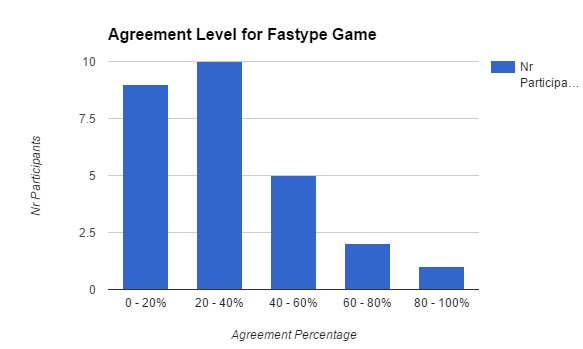
\includegraphics[width=\linewidth]{figures/experiment2/ex2-agreementlevel.PNG}
    \caption{Participant's Agreement Level for Experiment 2}
    \label{fig:game-agreement-level}
\end{figure}

\subsection{Game Design Analysis}
In the previous sub-sections we reported on the performances of non-expert human annotators in terms of annotation quality and agreement level and saw that the quality of annotations did not experience any decrease. In this subsection we report on the performance of Fastype in terms of playfulness, player engagement and see if the players were intrinsically motivated to participate and play the game. 

One of the metrics used to assess the playfulness or the attractiveness of both interfaces (AnnotateMe and Fastype) was by measuring the number of the so-called \textit{free-will annotations}. When conducting each experiment, the participants were instructed to perform their tasks continuously until instructed to stop. An annotation was considered to be a \textit{free-will annotation} when participants free-willingly decided to continue performing tasks even after the experimenter informed them that they have already completed the number of obligatory annotations and were allowed to finish the experiment. Table \ref{tab:free-will-annotation-res} shows the results of free-will annotations performed in both experiments in addition to the average number of tasks performed in a session. The game exhibits a slight improvement over the plain interface in terms of free-will annotations, however, the calculation of one-way Anova resulted in statistically insignificant difference for p = 0.05. The reason for the insignificant difference can be explained by observing the second row of the table, namely, the average annotations performed during an experiment session. We observe that participants performed 50\% more annotations using the plain interface as opposed to the game. Besides the fact that the difference was not significant, we argue that an average of 23\% free-will annotations over an average of 10 game rounds performed by a single participants is better than an average of 17\% free-will annotations over an average of 22 annotation rounds. In a long run, we are confident that the game would perform significantly better and have a significant higher attractiveness as compared to the plain interface. The results presented in Figure \ref{fig:participants-perference} easily back up this claim. 

% Table generated by Excel2LaTeX from sheet 'Sheet6'
\begin{table}[htbp]
  \centering
  \caption{Results of free-will annotations for experiment 1 and 2}
    \begin{tabular}{|l|r|r|}
    \toprule
    \multicolumn{3}{|c|}{\textbf{Participant Average Freewill and total annotations performed}} \\
    \midrule
          & \multicolumn{1}{l|}{\textbf{Fastype Game}} & \multicolumn{1}{l|}{\textbf{AnnotateMe Interface}} \\
    \midrule
    \textbf{Average of free-will annotations} & 23\%    & 17\% \\
    \midrule
    \textbf{Average annotations performed} & 10    & 22 \\
    \bottomrule
    \end{tabular}%
  \label{tab:free-will-annotation-res}%
\end{table}%


\begin{figure}[]
    \centering
    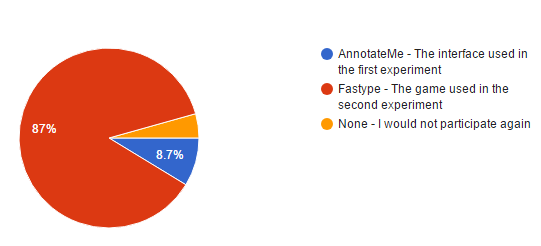
\includegraphics[width=\linewidth]{figures/experiment2/participant-preferance.PNG}
    \caption{Participant's preferred interface for performing annotations}
    \label{fig:participants-perference}
\end{figure}

After both experiments were conducted, we asked participants that took part in both experiments to fill-in a final questionnaire regarding their preferred interface in case they would be asked to do a third experiment. As seen from Figure \ref{fig:participants-perference}, the majority of participants preferred the game compared to AnnotateMe Interface. Please note that the participants had the possibility to choose a third option which allowed participants to express feelings of neutrality or dislike for both interfaces. The third option was provided as a measure against potential bias in our results by allowing all participants who disliked both experience to freely express it. The questionnaire was completely anonymous and was sent through emails where participants completed it from home.

%Post Questionnaire
A post-questionnaire assessing the overall design of the game was also used in the second experiment. In the post-questionnaire, participants were asked different type of questions with each contributing to the assessment of different aspects of game design. Additionally, in order to compare the attractiveness and engagement of participants with the game and the plain interface, both designs were assessed using similar questions in both post-questionnaires. 

%Anova analysis towards experience with interfaces
In order to assess the attractiveness of each interface we asked participants to rate their experience with each interface. The results of the first experiment are shown in the top-right graph presented in Figure \ref{fig:ex1-postresults} whereas the results of the second experiment are presented in Figure \ref{fig:game-experience}. To make sure that the game was perceived as significantly more attractive and fun to use as compared to the plain interface, we run one-way Anova analysis and the results confirm that the difference is statistically significant for p = 0.05 and for p = 0.01. This indicates that the game was perceived significantly more attractive as opposed to the plain interface.

\begin{figure}[]
    \centering
    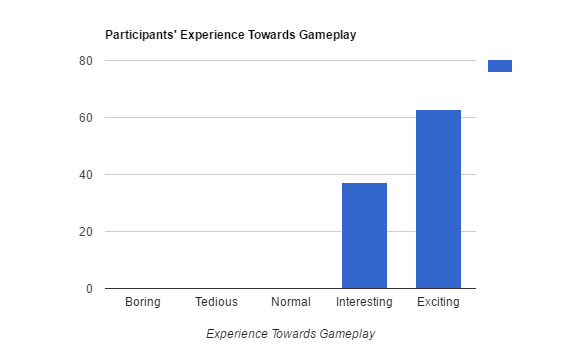
\includegraphics[width=\linewidth]{figures/experiment2/game-participant-experience.PNG}
    \caption{Participant's experience towards the gameplay}
    \label{fig:game-experience}
\end{figure}

%anova analysis about egagement frequency
Regarding the user's perceived engagement with both interfaces, we asked participants how often they would use each interface outside the experiment. Please note that for the same question we unfortunately used different type of answers, with the answer for the first experiment being labels ranging from "Definitely Not" to "Definitely", and the answer for the second experiment being a 7-point liker scale ranging from "Never Again" to "A Lot". However, when calculating one-way Anova, we normalized the 7-point liker scale to 5-point liker scale (dividing the value with 7 and than multiplying it with 5) to be able to properly compare the two observations together (See Appendix \ref{appendix3:engagement_analysis}). The results of the one-way Anova report a statistically significant difference between the two observation for p = 0.05 as well as p = 0.05. These results indicate that the game was perceived as significantly more engaging than the plain interface.  


\begin{figure}[]
    \centering
    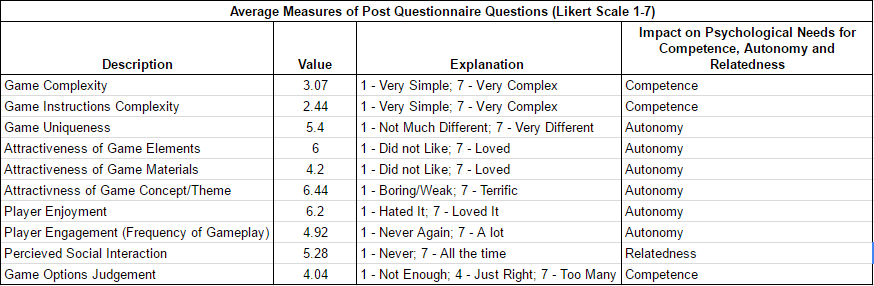
\includegraphics[width=\linewidth]{figures/experiment2/post-questionnaire-final.PNG}
    \caption{Results from the post-questionnaire analysis for experiment 2}
    \label{fig:post-questionnaire-final}
\end{figure}

Finally, Figure \ref{fig:post-questionnaire-final} presents a table with the final results for the rest of the questions used to assess the design of the game on the post-questionnaire. It can be observed that the game scores relatively well in all of the design questions presented to the participants. The table also illustrates the impact of the different game design elements on basic psychological needs for autonomy, competence and relatedness which represent the main factors for affecting player's intrinsic motivation. Since the players perceived the game as generally enjoyable, engaging, socially intractable, easy to adapt with the instruction and rules of the game, genuinely liked the elements, materials and the theme of the game, we claim that the participants were intrinsically motivated to play and do not rely in any other incentive but the desire to be entertained. Consequently, based on these acquired results the first hypothesis of the second experiment is supported (H2.1). The second hypothesis (H2.2) is also supported since the one-way Anova analysis indicate that the participants preferred to use the game significantly more than using the plain interface.  
\chapter{Discussions}
\label{chap:discussions}

Named entity linking and disambiguation has been a problem for which many studies have tried to find an effective solution either by using automatic supervised algorithms or utilizing human input for validation and generation of annotation data \cite{39, 9, dbpedia, 16, 31}. Despite the advancement of supervised techniques using machine learning algorithms, tasks such as \ac{ned} and \ac{wsd} still haven not reached a satisfactory performance for generating trustful data quality \cite{30}. Relying on human input for validating these automatic approaches has been seen as the only way for progressing in this aspect. A question which has drawn constant attention is whether non-expert human annotators are capable of generating annotations with a quality comparable to expert annotations. The implementation of a complete \ac{ned} framework which was used to generate annotations using non-expert annotators in an experimental setup reveal that these users are capable of generating annotations with an accuracy of 0.92 (F-score).


\section{A framework that supports qualitative annotations}
These findings are complementary with previous work which also tested the ability of non-expert users to perform tasks for \ac{ned} and \ac{wsd} \cite{14,16,9,32}. However, previous human centered approaches for \ac{ned} were either focused on assessing the usability of their interfaces \cite{15,16,17} or they used human annotators for temporarily validating automatic generated data without utilizing such power in the future \cite{31,32,33}. On the other hand, automatic supervised and unsupervised techniques for \ac{ned} have implemented complete systems with some of them performing relatively well \cite{39, 21}. With the implementation of a loosely coupled microservice architectural framework that utilizes the best systems and techniques from the automatic approaches and usability best practices from human centered studies, this research study refines previous work by effectively combining these two approaches to get the most out of automation and using human input only in essential parts such as validating and disambiguation. Analysis and findings from the results acquired during experimental trials throughout this research project show that it is possible to rely on non-expert human annotators for generating qualitative data using the implemented framework. The generated data can be used to enrich HTML content with semantic data from \ac{lod} knowledge bases or train supervised approaches until they are mature enough to disregard human judgments.  

\section{Short clues as context representatives}
Among the reviewed human centered research studies, whether they used crowdsourcing or gamification for utilizing human validation, none of them had attempted to properly define or formalize contextual information in texts document in an automated way to assist human annotators on the disambiguation process. Supervised automatic algorithms on the other hand have formalized contextual information as features to feed in into the algorithms showed improvements on disambiguation performance \cite{24,29,33}. However, these contextual features are designed for intelligent algorithms and are not as helpful for human annotators. Therefore, this study extends on previous work by providing a service that can effectively generate contextual information surrounding the target entities which might help non-expert annotators easily disambiguate ambiguous entities. Our findings reveal that participants tend to prefer short contextual clues instead of complete sentences. However, because of limitations in the methodology chosen to assess the effectiveness of these clues, it was not possible to make such a claim that the clues generated by our service provide sufficient information for annotators to correctly disambiguate an entity. The main reason that resulted in choosing a rather poor and inappropriate evaluation methodology for assessing the effectiveness of contextual clues is the lack of time resources in conducting a third experiment. Therefore, we acknowledge the fact that asking the participants in the post-questionnaire whether the context clues were useful without actually testing this variable in a two-fold experimental setup was not the best methodology employed and it is considered a limitation to our study. 

However, when designing the game, this problem was solved by using another approach of feeding context to the user. In addition to the short contextual clues, users were additionally exposed with the complete sentence but in a way which does not overwhelm them and avoids redundant cognitive load. The design of the game task made it possible to use the sentence for communicating the context unconsciously by having the user type the complete sentence as part of a fun activity (fast typing). This proved to be significantly effective since the quality of annotation remained the same during the second experiment.

\if However, since the results show high levels of annotation quality and moderate agreement levels between participants, we assume that the contextual clues generated by our framework are significantly more user-friendly and exhibit significantly less cognitive load to the participant compared to showing complete sentences. At the end of the day, our goal was to keep users motivated and interested to contribute in generating annotations. Therefore, using long sentences as contextual clues would potentially result in negatively affecting the UI/UX of the interface and the player's motivation to play. \fi

\section{Gamifying non-gaming systems}
Since the results from the first experiment revealed that the micro-service architectural framework for \ac{ned} supports the generation of qualitative annotation by non-expert users, we have used this framework as a foundation on top of which a gamified system was build in order to intrinsically motivate users for contributing instead of using payment incentives like crowdsourcing \cite{9,32,33}. In general, our findings corroborate with previous work in gamification that game mechanics and game design principles can be applied in non-gaming context in order to make the task more engaging and fun to interact \cite{44,45,50}. Some research studies in gamification of annotation tasks for \ac{wsd} show that gamification helped in improving annotation quantity with no significant results in the improvement of annotation quality \cite{46}. Our results extend on these previous work that gamification can be used for not only increasing annotation quantity but also maintain high levels of quality. By observing and analyzing the results of our study, we continute to support the idea that applying game elements in non-gaming context does not necessarily motivate users and improve quality and quantity of annotations unless psychological needs for intrinsic motivation are satisfied.

\section{Limitations}
Results from the second experiment reveal that the game mechanics and the overall design of the game positively affected users needs satisfaction and intrinsic motivation to contribute. However, it is important to address that there might be some potential bias in assessing the users initial motivation to participate in the study. In our experiment, we recruited participants that were mainly bachelor or master degree students studying at the university campus. It is known from previous research studies that participants from the university usually engage voluntarily in studies and it is possible that they already had a minimum level of intrinsic motivation from the get-go effect, which might have affected the results. Additionally, the population used in the experiment consisted of students with higher education in the field of computer science, information security and interaction design. Thus, one might argue that the label "non-expert annotators" cannot be applied to this type of population. However, the game was designed in a way that every player, regardless of their educational background, had to go through the onboarding process which is a gamified version of a training stage and assures that players understand the game elements by slowly exploring the complexity of the game. Besides the fact that we were limited in the type of population that was available to conduct the study with, we stay behind our claims that the framework and the game design supports the generation of qualitative annotations by non-expert users. Despite the acquired significant results and our confidence in generating qualitative annotations with the population at hand, more research is required to investigate how users' initial motivation to engage in gamified application affects their subsequent motivation and also test the game with users that better represent the general target population\cite{46}.

\section{Practical and theoretical implications}
The main lesson learned from applying the gamification process to the named entity disambiguation framework is that game design can be applied to any non-gaming contexts as long as the design conforms to empirical and psychological foundations with all game elements directly or indirectly contributing to the solution of the problem at hand. The real challenge in designing a game with a purpose is finding a model that is appropriate for the task but also contributes to user engagement and intrinsic motivation. Controlling players for malicious behaviour, maintaining players within the defined flow-zone of game complexity, providing meaningful content, non-formal feedback that is visually and aurally attractive without shifting the players concentration and focus from the main task are aspects which when appropriately addressed, contribute a great deal towards having an enjoyable \ac{gwap}. In Fastype, all the game elements contribute to the general idea of providing qualitative annotations and each game element plays an important role in helping players make correct disambiguation decisions. Designing a game that encourages competitive players to unleash their competitive nature into the gameplay while also providing a safe game environment for players that prefer to play safe without taking risks are additional game design factors that characterize a well-thought \ac{gwap}. Though, some research studies which have investigated on gamifing WSD and entity linking argue that text-based games are limited in their potential compared to 2d video-games, our results conflict with these claims \cite{54}. This research work, based on statistically significant results, rejects the claims stated by Vannella et al. \cite{52} by proving that even text-based \ac{gwap} can be as engaging and entertaining as 2D video-games when it comes to truly engaging a player.
\chapter{Conclusion and Future Work}
\label{chap:conclusion}

% MN: Try to separate the 3 aspects of your work:
% 1. Research. The research questions are answered by the data that you have collected. 
% 2. Engineering. The data that you can collect is because you have constructed (engineered) a tool (or set of tools).
% 3. Design, Architecture and Construction. This is related to point 2, but, it is the decisions, the architecture, the game design, the balancing, the choices of frameworks, methods, flows, etc. All the "choices" that you had to make first, before point 2 can take it and "build it".  
% Point 2 is BSc work. Engineering. "Boring" or "Mundane". Sure, it was part of your work, but, give it 3rd, last place in discussions.
% Point 1 is your primary objective. Posing, and answering research questions. This is what MSc process is all about. 
% Point 3 is huge part of your work, and, of course, fundamental to get to point 1. But, it is still "a tool". So, it comes on the 2nd place. The first place is point 1.

% So, below, when you drawing conclusions, you have to make sure the reviewer is clear, if you are discussing point 1, or point 3, and why. Do not mix them. When you have research question that requires data, statistics, and the conclusion is drawn from the data and stats, keep it simple. Just write about that. Logical.   Keep arguing your case with data.  Not with "construction".


% Then, as an added value, added contribution, describe the construction. Point out, that you have, beside the research questions and answers, done work in solving architectural and design decisions, and they contribute to the quality of the overall work. But, try not to mix "research" with "construction". It will read better, and it will be easier to follow by the reviewers.



The focus of this research has been primarily on investigating gamification and games with a purpose for facilitating data gathering processes for named entity disambiguation (NED). To assure fast and reliable inter-communication between a gamified system and another system that carries out the complete automated process of entity disambiguation, a framework of our own was deemed necessary to be implemented as part of this study. The implementation of a microservice architectural framework with state-of-art utilized techniques for NED and the implementation of a complete gamified system which utilizes the output from all components of the framework represent the concrete contributions of this work. In order to test the effectiveness of this proposed approach to NED, two user experiments have been conducted. The results acquired from analyzing the data generated from the user experiments, statistically support some of the claims hypothesized by this study and helped answer the posed research questions which are individually addressed below.  \hfill \break

% State the major conclusions from your study and present the theoretical and practical implications of your study.


%ANSWER YOUR RESEACH QUESTIONS 

%User present tense when talking about facts

%User past tense or present perfect when when refering to the research done 

%Do not use first person, interpret new issues, provide new information, use examples, cut and paste passages from the results 

 \textbf{How accurate can an entity disambiguation framework, by using human input, validate the automatic linking process of named entities with knowledge bases?}\hfill \break

In order to answer the first research question, the effectiveness and usability of the information generated by the microservices had been tested through an experimental user study with non-expert participants validating links generated from the framework. For this purpose, AnnotateMe was implemented as a front-end interface to engage with participants by providing all the necessary information for the correct disambiguation to take place. \if Additionally, gold standard datasets where used as corpus for feeding in into the framework to be validated by the users. Since the gold standard provided the correct answers for each individual entity available in the datasets,we were able to assess the quality of the generated annotations by the non-expert annotators.\fi Statistically significant results indicate that the information generated by the microservice components of the framework support the generation of high quality annotation data by non-expert annotators with an accuracy (f-score) of 0.92. 

\if Having implemented a framework that supported quality of data at such high levels was crucial before starting the gamification process. However, since the framework consisted of novel implementations, specifically targeting the component which is responsible for generating contextual clues to help disambiguation, a scientific assessment of the usability of these contextual clues generated by the framework was mandatory. The second research question addresses the concerns about the effectiveness of contextual clues with regards to entity disambiguation.\fi \hfill \break
    
\textbf{What features can be used to formulate the context surrounding entities so that non-expert users can correctly disambiguate them?}  \hfill \break

\ac{nlp} is among the many research fields which have investigated in potential methods for defining context in a textual representative way~\cite{22}. The appropriate formulation of context solemnly depends on the task and target (human or machine) who makes use of it. This research study was concerned in finding features that would be appropriate and helpful to help non-expert users to easily grasp the context in which the entity occurs and correctly disambiguate it with the appropriate candidate. Proximity features such as bi-gram collocations, neighbor entity mentions and topical document keywords are the features that this study has experimented with. Statistical analysis of the results acquired from the first non-gamified experiment show that these contextual clues (features) proved to be helpful in the overall disambiguation process. However, as a result of insufficient data gathered during the experimental studies and the selection of a rather inappropriate assessment methodology for the effectiveness of the contextual clues resulted in acquiring statistically insignificant claims. We account this as a limitation of our study and address improvements for future work.\hfill \break

\if The effectiveness of these features was only measured using assessment questions from a post questionnaire where participants were asked to rate the usefulness of the clues with regards to the disambiguation process. Therefore, insignificant statistical results were acquired as a side effect of applying insufficient assessment methods for measuring the corresponding effectiveness of the designed context features.\fi


\textbf{What game mechanics can be employed in the entity disambiguation task so that high levels of engagement are achieved while still maintaining annotation quality?}  \hfill \break

The idea of applying game elements into non-gaming contexts with the purpose of solving a particular problem (\ac{gwap}) has been researched across many domains \cite{47}. A recent literature survey conducted by Seaborn et al \cite{45} shows that the majority of studies that have applied gamification did not base their work on empirical and theoretical foundations. The game design of Fastype has been entirely based on theoretical and psychological foundations. 

This research study hypothesized that the game elements applied to the \ac{ned} framework would hide the boring nature of the actual task and emphasize the entertaining and fun aspects of the game which in turn leads to the users being intrinsically motivated. Since the third research question is concerned in discovering the underlying game mechanics for reaching the respective state of being intrinsically motivated, the results of the study suggest applying the following game mechanics for a successful \ac{gwap}: 
\begin{itemize}
    \item Onboarding
    \item Triangularity (supporting both players who like to take risks and those who like to play safe)
    \item Non-Formal and visually appealing feedback
    \item Appropriately and dynamically adjusting game complexity as the player advances through the levels (maintaining game flow)
    \item Controlling for malicious player behaviour and maintaining gameplay quality
    \item Social interaction mechanisms within the game
    \item A well defined game engagement loop which motivates emotion, assures re-egagement with the game, provides social call to action and makes the progress of players socially visible
\end{itemize}
\if This research study opposes to some previous research work \cite{54} by showing that textual interactive-based GWAP can be as fun and entertaining as video-based GWAP. Statistically significant results prove that the game mechanics applied to the NED framework engaged participants significantly more than compared to using non-gamified interfaces, and as a result, participants were intrinsically motivated to participate. In terms of annotation quality, the gamified version of NED Framework did not have any negative impact and therefore annotation quality remained stable.\fi


The work and results reported by this research study have theoretical and practical implications in the respective field. This research study contributes to perishing the doubt of \ac{gwap} being successfully and effectively applied in non-gameing contexts. As long as the design of the game is based on empirical foundations and other psychological factors that impact human intrinsic motivation, the success is easily achievable. Providing novel approaches for effectively and efficiently improving named entity disambiguation systems results in continuous improvements in the areas of information retrieval systems and semantic web respectively \cite{12}. It is this sort of research work that devises techniques which can substantially improve efficiency and scalability while retaining high quality and accuracy of data. \hfill \break


\textbf{Future Work}  \hfill \break

% MN: Make the "larger sample size" a last, additional point. 

% MN: Start with the improvements to the tests that would strengthen your results in the context of gamification effectiveness. What future tests could you suggest that could improve the "game" aspects? What have you learned but still do not have sufficient evidence for? Imagine that 4 other MSc students want to continue your work, what research questions could be given to them to investigate? 

% MN: Then, change gears, and talk about "technology". Then mention improvements to the framework, additional micro services or other engineering and technological contributions. 

In terms of future work, there are some aspects that could be further improved and some of the claims further strengthened. First and foremost, in absence of the possibility to test the system with a broader and more general population during the period of this research work, it is necessary to conduct another experimental user study with strong focus on having a larger representative sample of the general population. 

Additionally, the conducted assessment methodology for evaluating the effectiveness of contextual clues with regards to effective disambiguation, a two-fold experimental user study should be conducted in the future. A two-fold experimental study with the control group being exposed with the complete sentence as contextual clue and the experimental group being exposed with short context clues extracted from the framework would improve the validity of the methodology used to evaluate the effectiveness of contextual clues. Being timely constraint, conducting such experimental trial is left out for future work.

Finally, with the implementation of an additional microservice which integrates semantic meta-data in the form of RDFa for unstructured HTML5 documents would increase the contributions of this work~\cite{rdfa}. Having RDFa data attached as semantic information for each entity present in a web document would potentially extend the meaning of the web documents making them semantically more machine-readable. Another interesting future direction would be incorporating this framework for gathering data for other complex \ac{nlp} problems such as \ac{wsd}. 
%END OF CHAPTER IMPORT


\ifthenelse{\boolean{HarvardCitations}}{%
	\bibliographystyle{agsm} % used for Harvard style references. Names - Humanities & Interaction Design
}{%
	\bibliographystyle{ntnuthesis/ntnuthesis} %used for Vancover style references. Numbers - Computer Science & Physics
}

%Bibliography
\bibliography{MastersExample}

%Appendices
\appendix
\chapter{Experiment 1 - AnnotateMe}
\label{appendix1:annotatme}

\section{Documentation of RabbitMQ Message Routes}
\label{appendix1:AMQPDOCsec}
The table below represents all the communication infrastructure for the asynchronous publish-subscribe messages protocol. All microservices composing the NED Framework exchange information with each other by publishing and subscribing to each-others' message queues using RabbitMQ as the underlying technology provider. All the parameters associated with each communication route (Routing Key - Column 1), are mandatory and shall be provided as a complete JSON object with the specified name and the corresponding data type.
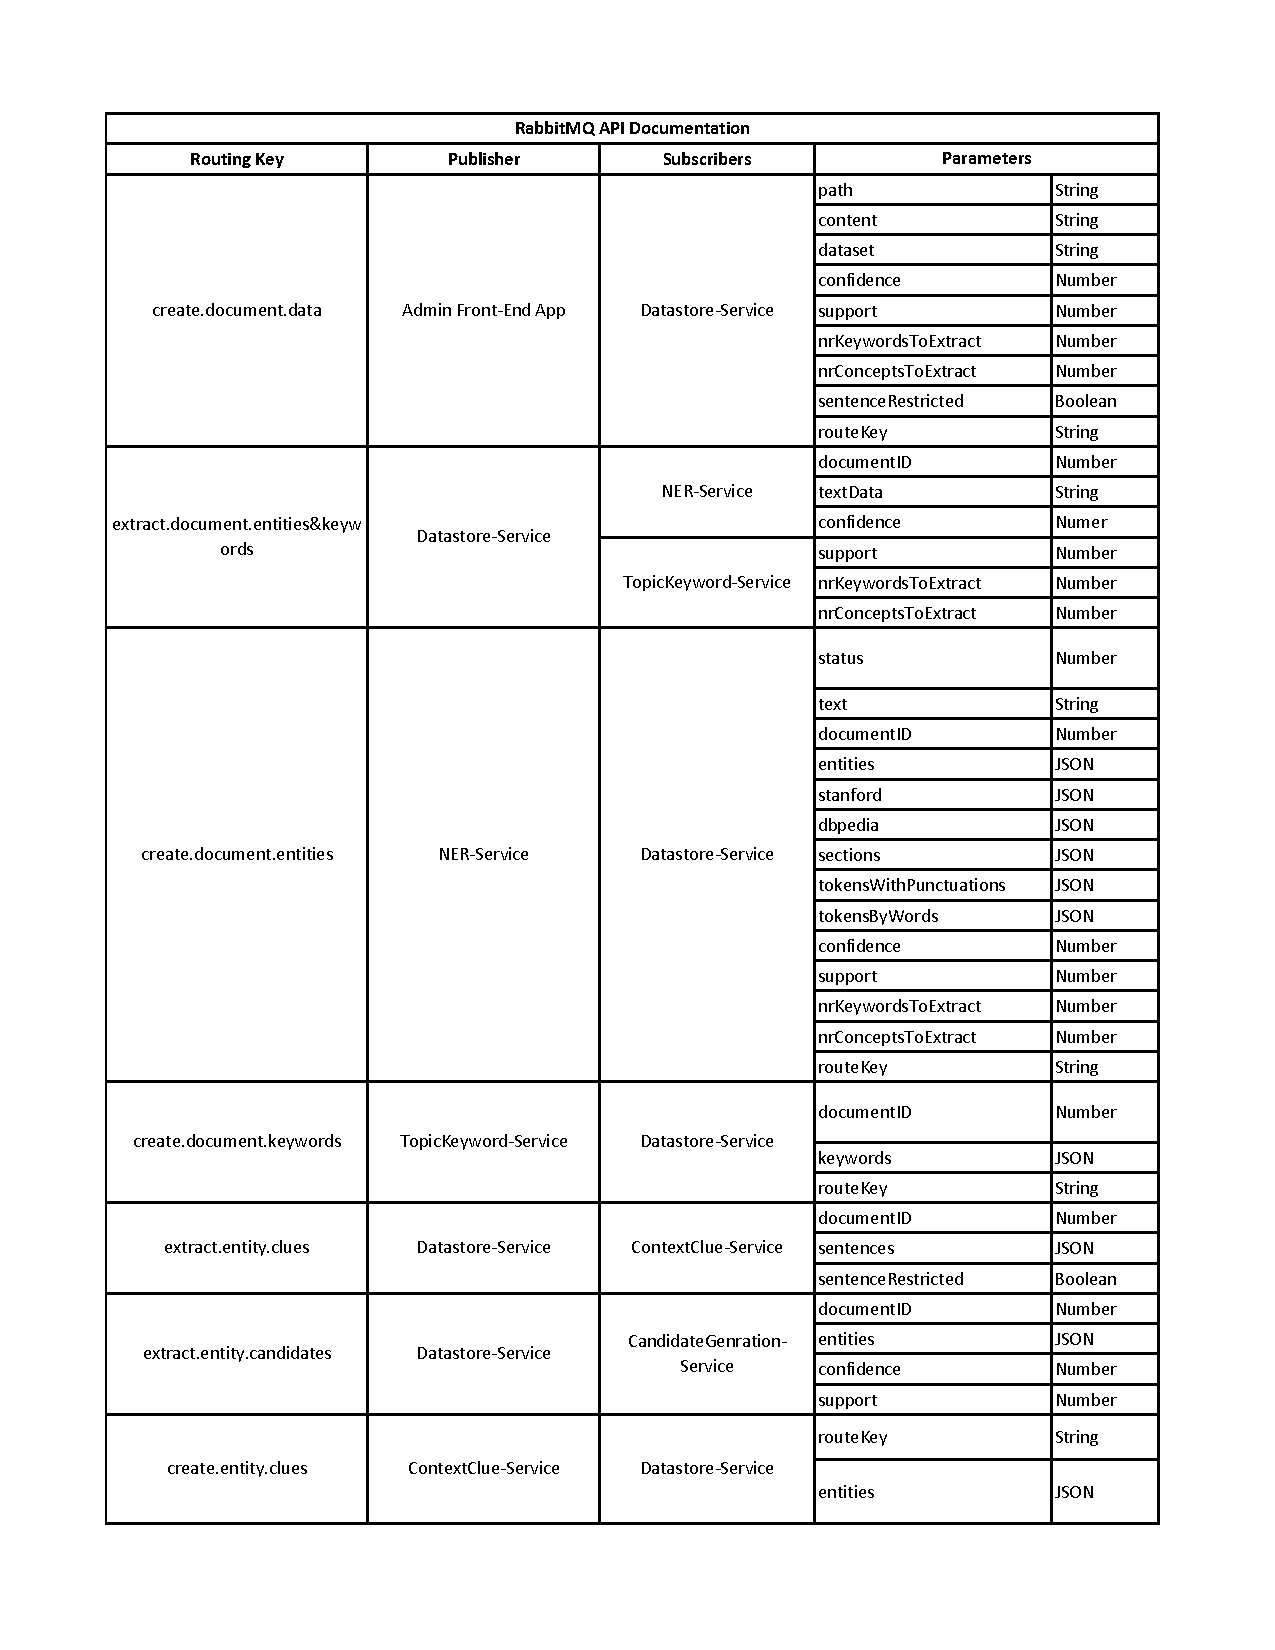
\includepdf[scale=0.7,pages=-]{appendices/rabbitmq-doc.pdf}

\section{Documentation of Datastore and Dataprep Microservice REST routes}
\label{appendix1:RESTDOCsec}
This appendix documents all the routes used to access the resources residing in the \textbf{Datastore Microservice} as well as the documented routes for accessing resources from the \textbf{Dataprep Microservice}. Swagger Documentation API\footnote{Swagger IO \url{http://swagger.io/}} has been used for generating the documentation schema illustrated below.

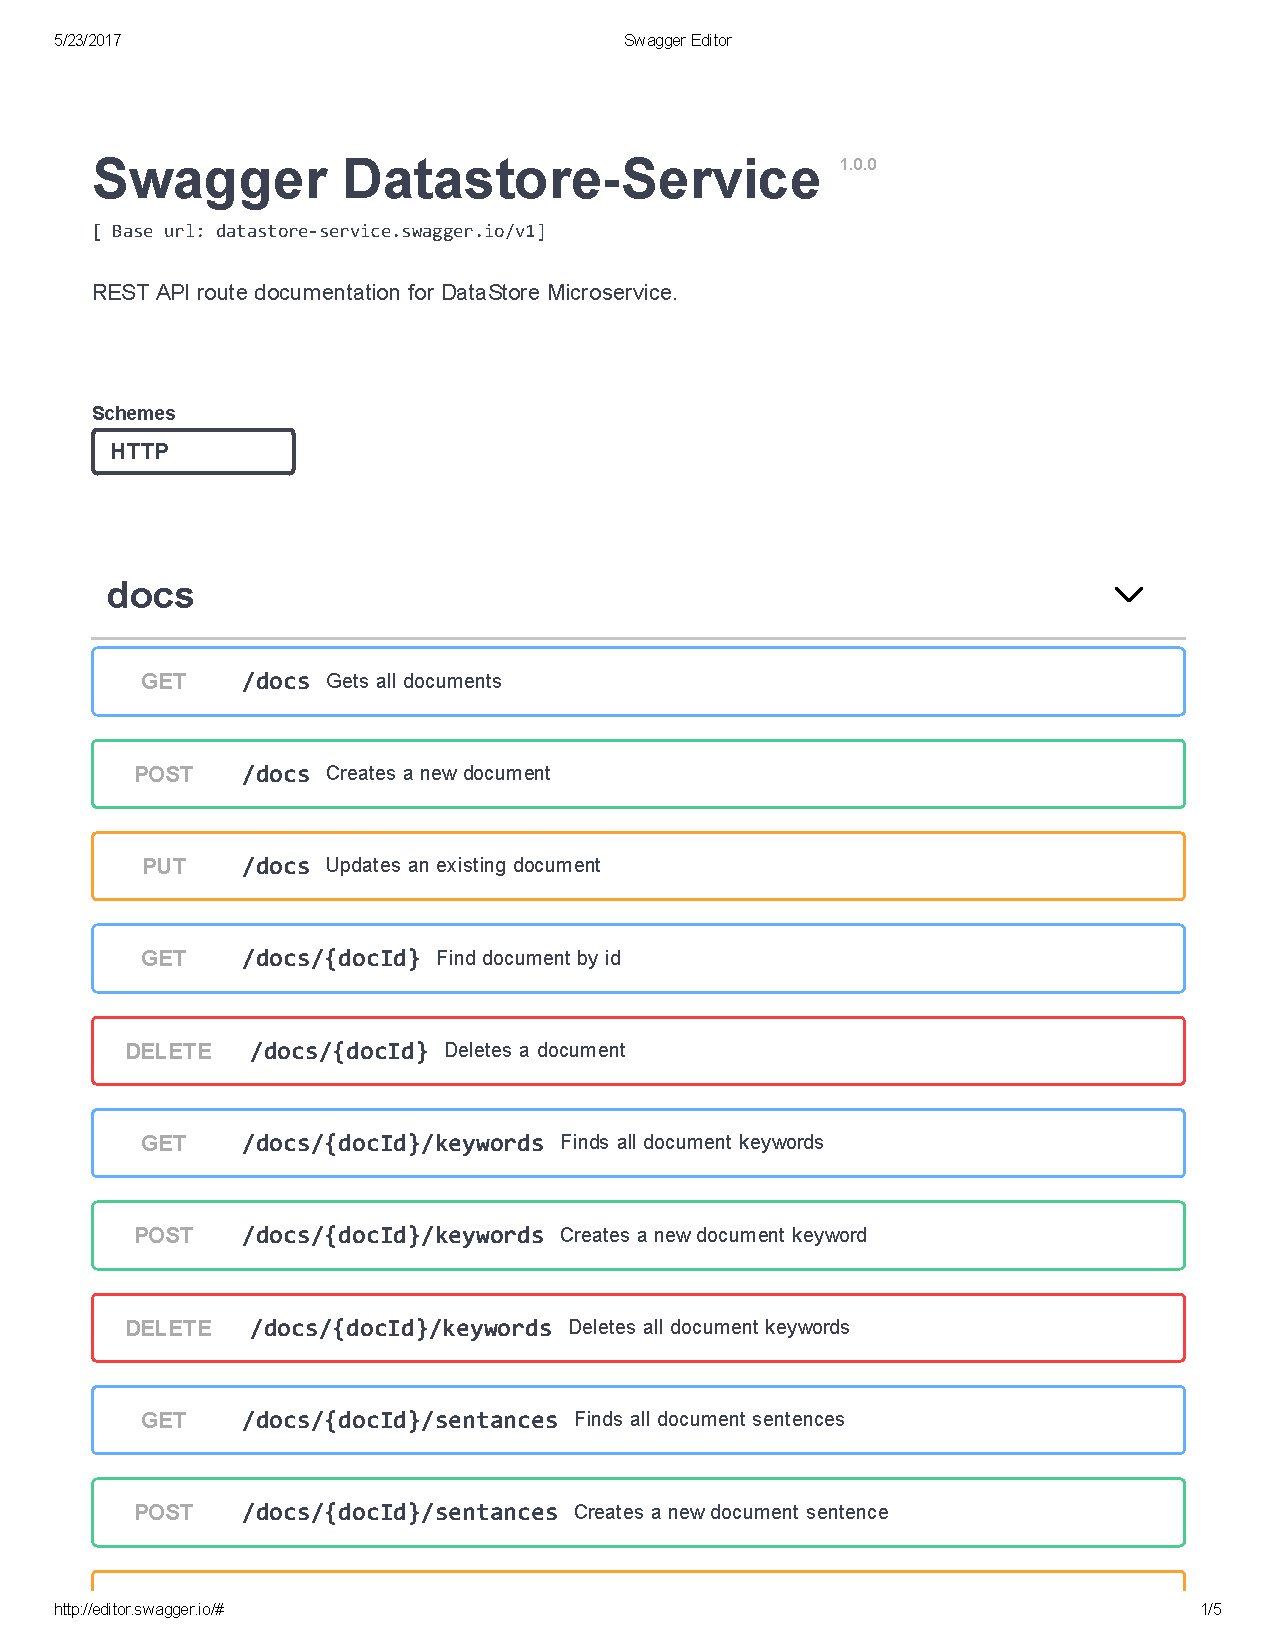
\includepdf[scale=0.7,pages=-]{appendices/swagger-datastore-service-documentations.pdf}
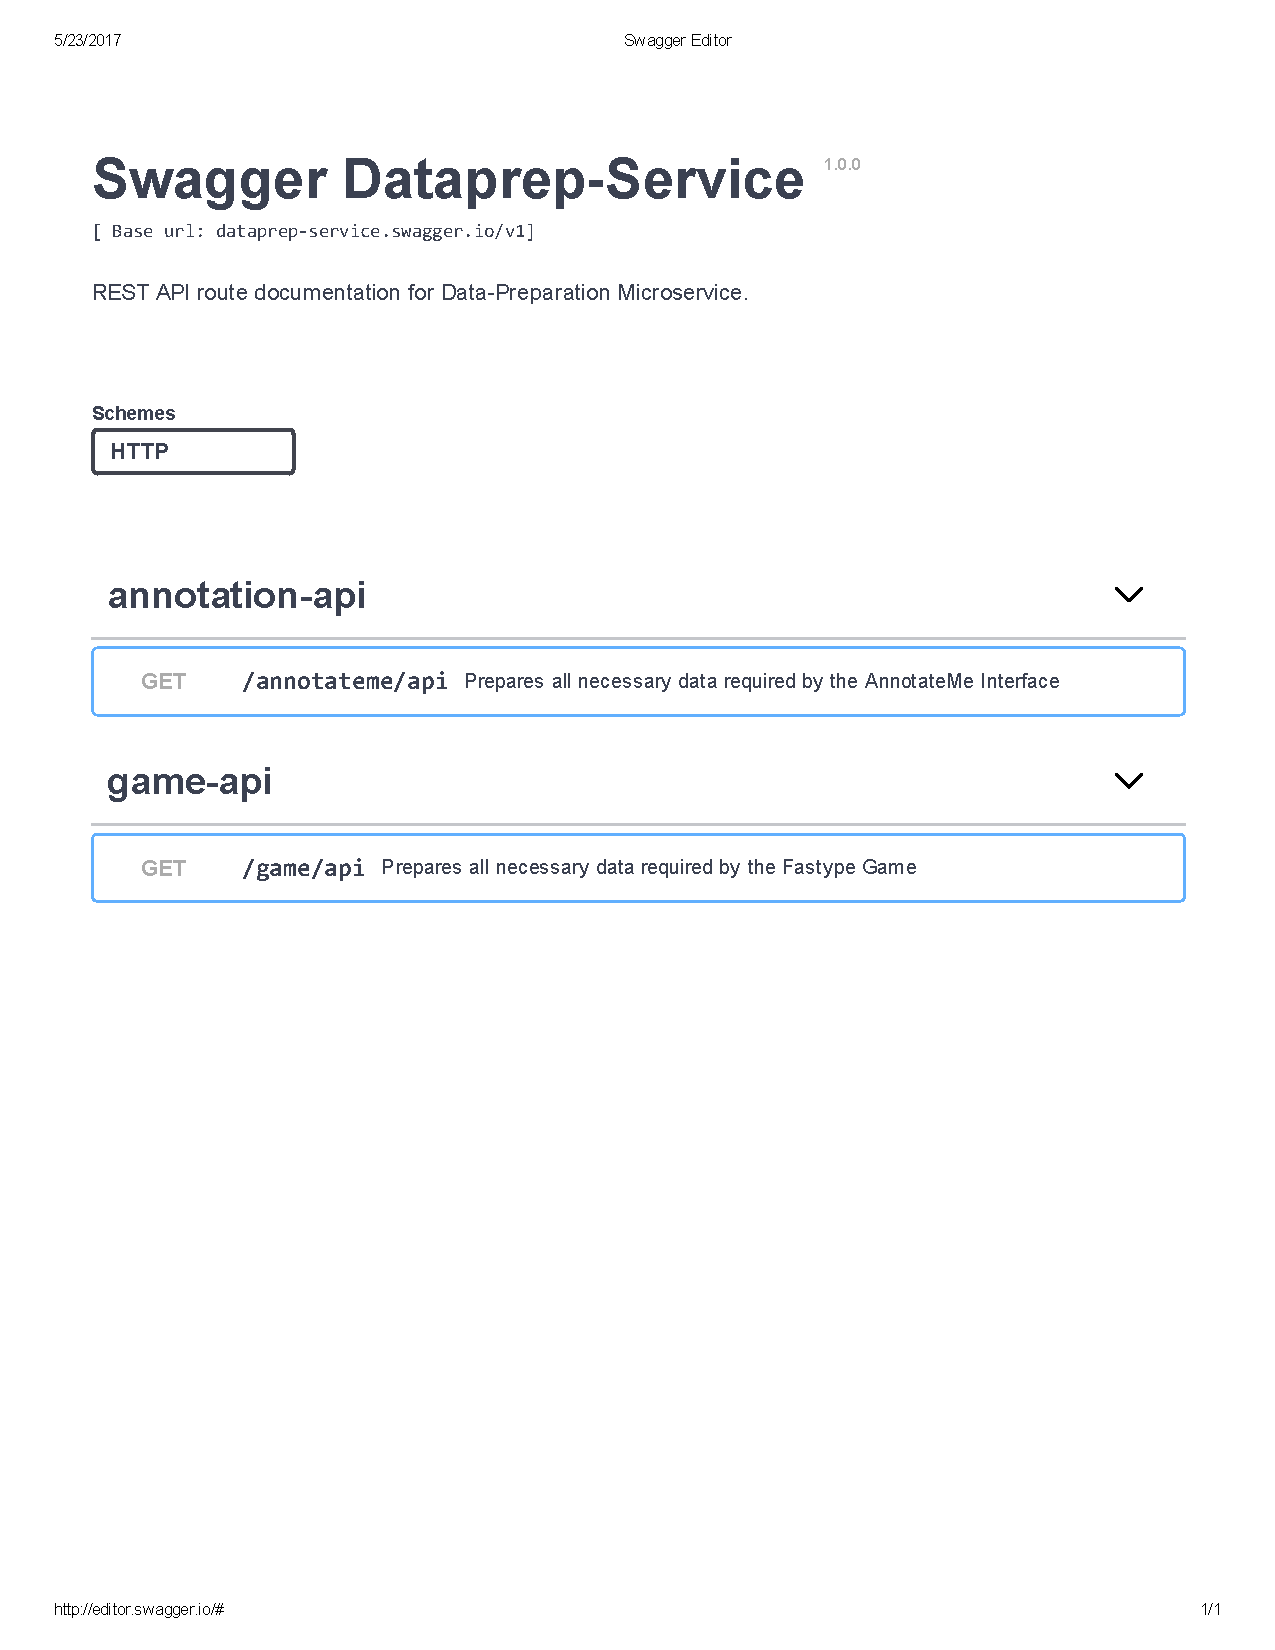
\includepdf[scale=0.7,pages=-]{appendices/swagger-dataprep-service-documentations.pdf}


%Ex1 - Consent Form
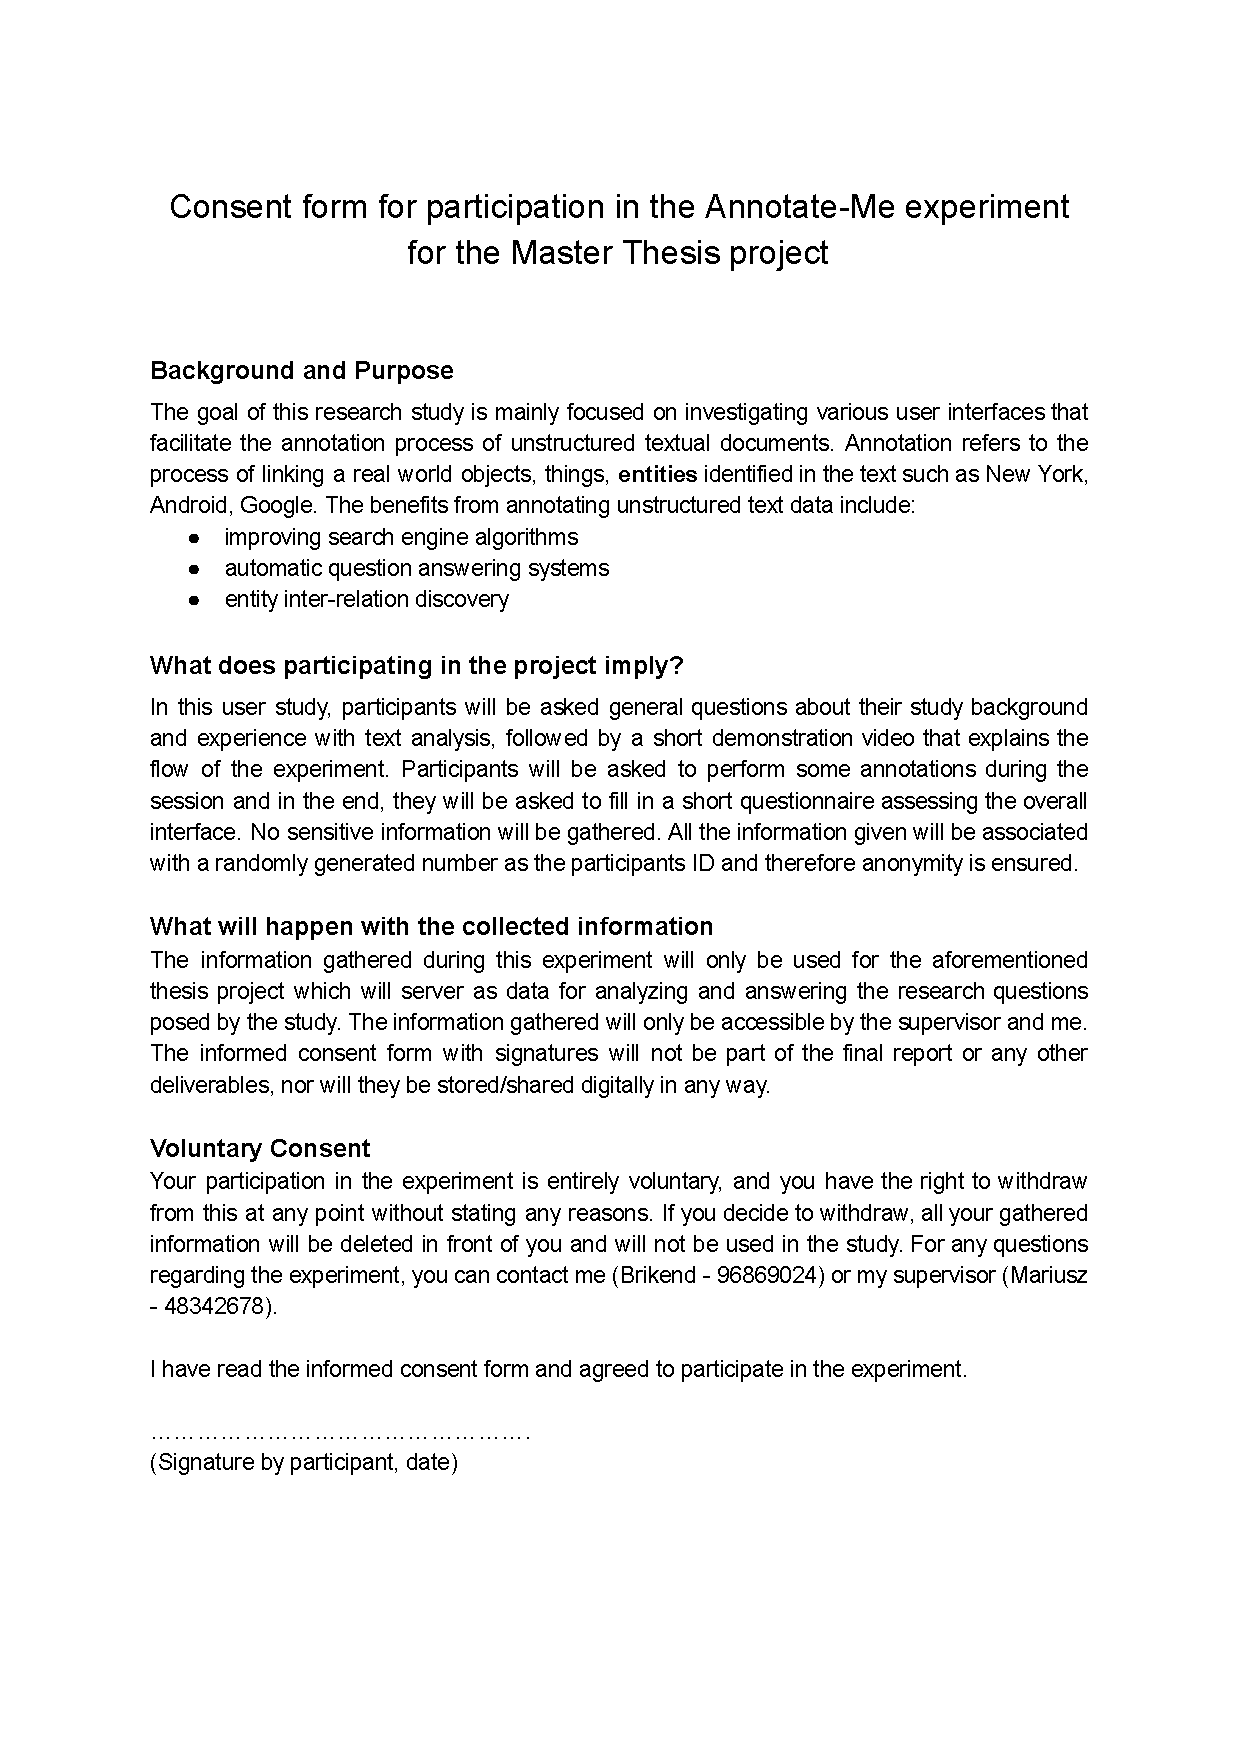
\includepdf[scale=0.8,pages=1,pagecommand=\section{Consent Form}]{appendices/experiment1-consentform.pdf}

%Ex1 - Pre Questionnaire
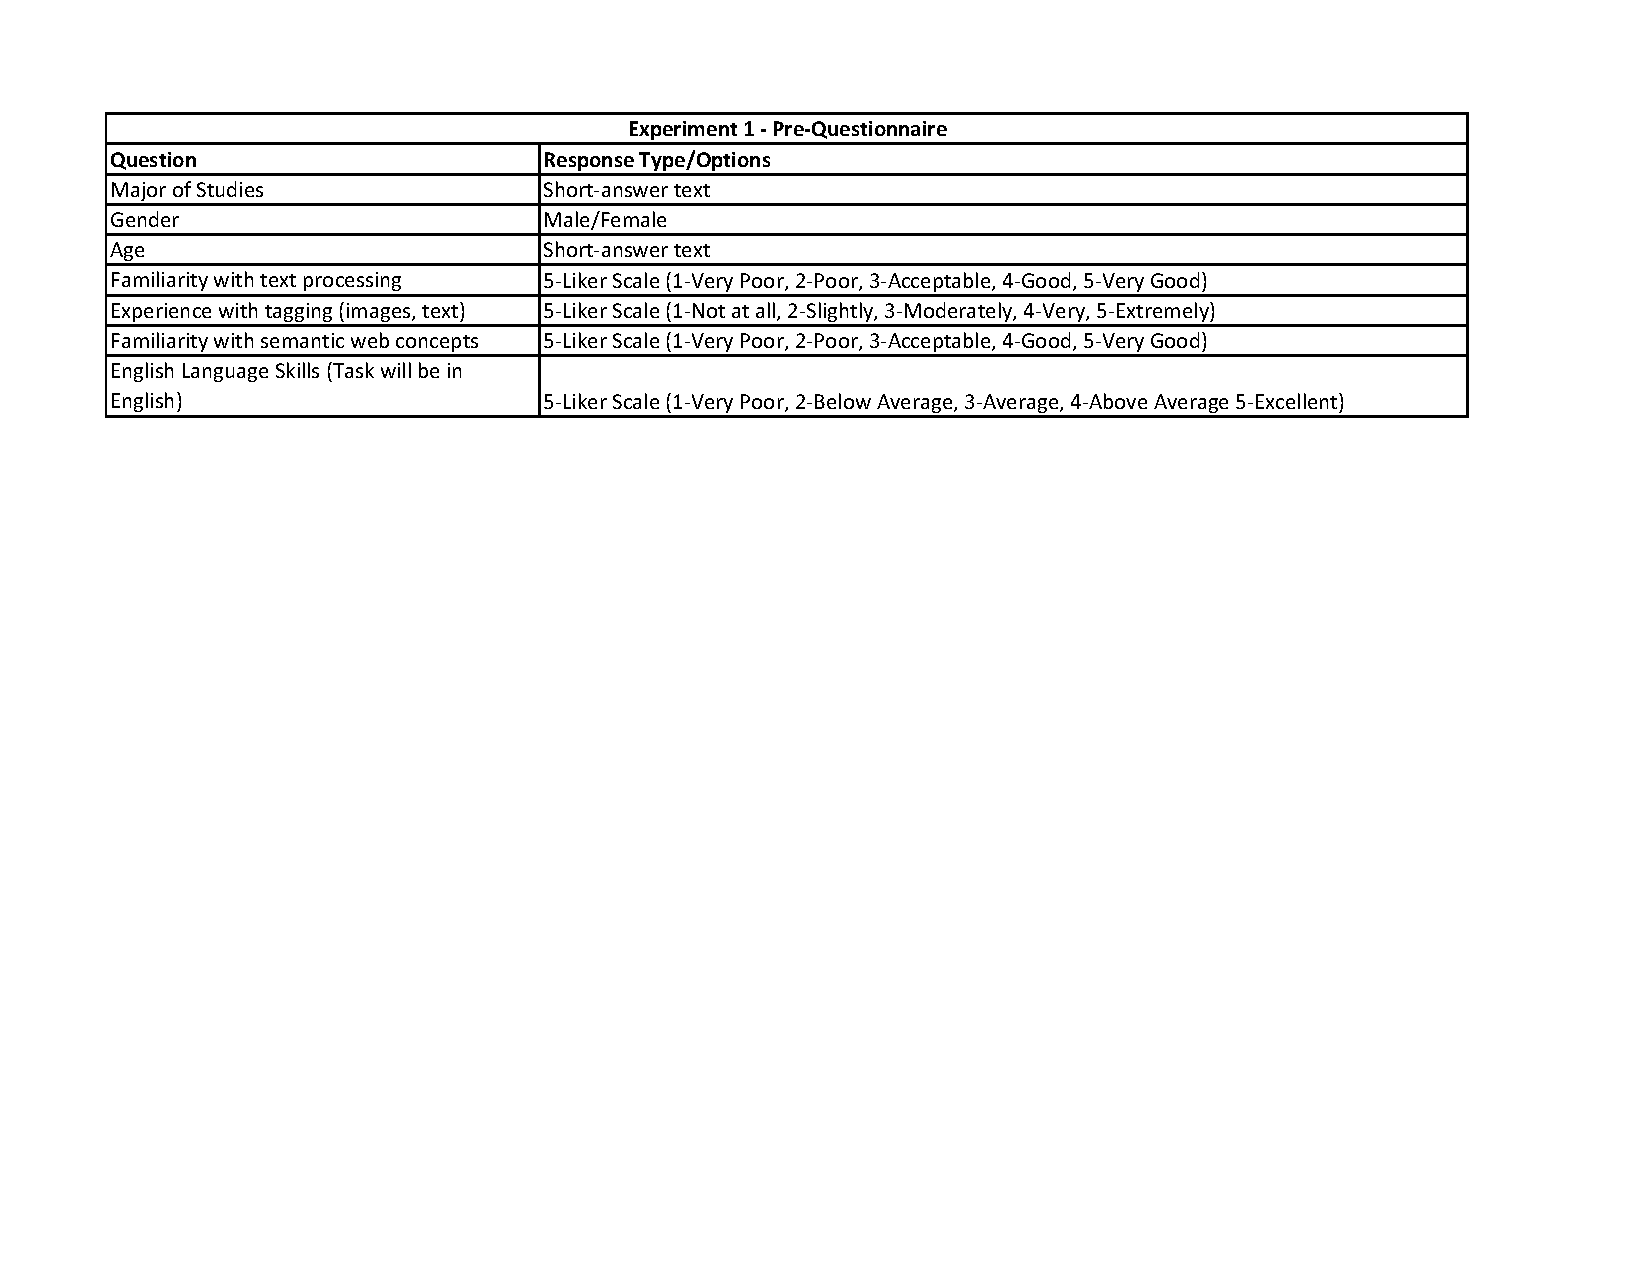
\includepdf[scale=0.8,angle=90,pagecommand=\section{Pre-Questionnaire }]{appendices/pre-questionnaire.pdf}

%Ex2 - Post Questionnaire
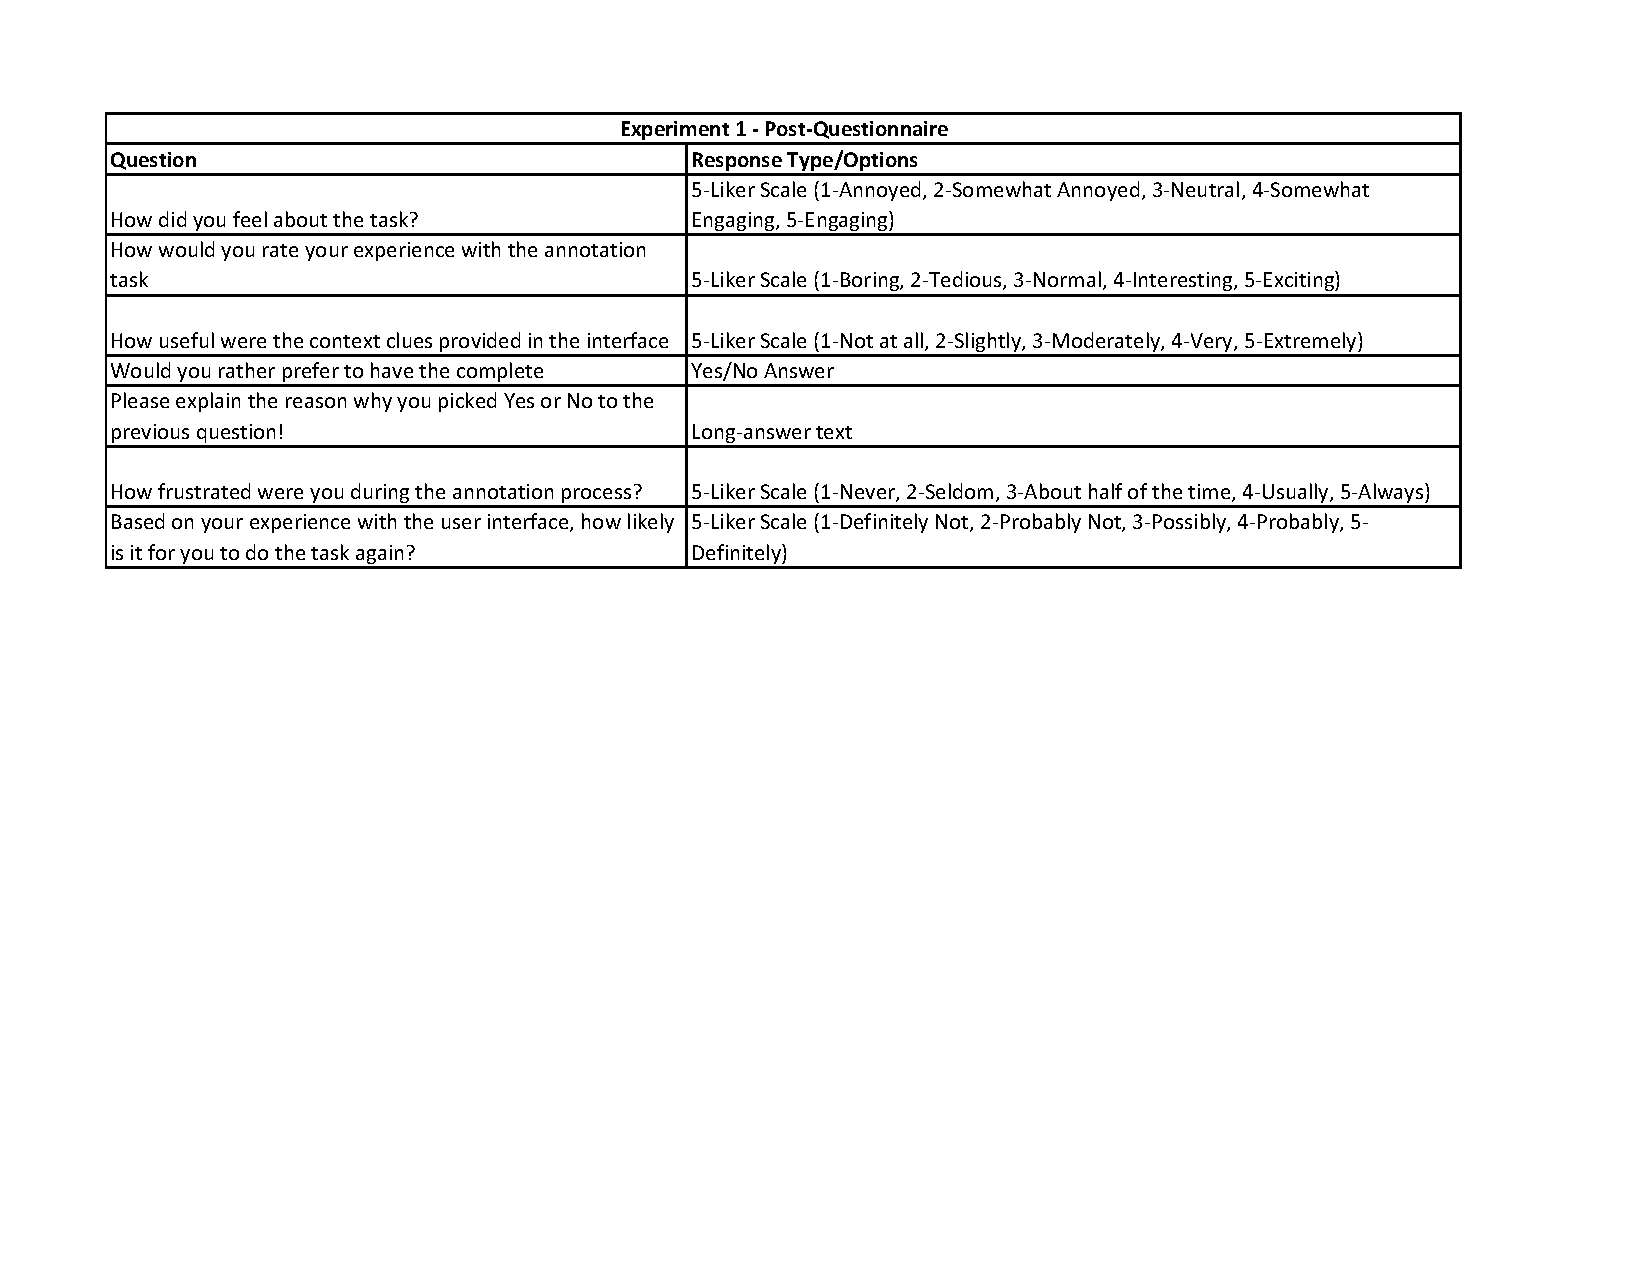
\includepdf[scale=0.8,angle=90,pagecommand=\section{Post-Qestionnaire }]{appendices/ex1-postquestionnaire.pdf}

\chapter{Experiment 2 - Fastype}
\label{appendix2:fastype}

%Ex2 - Consent Form
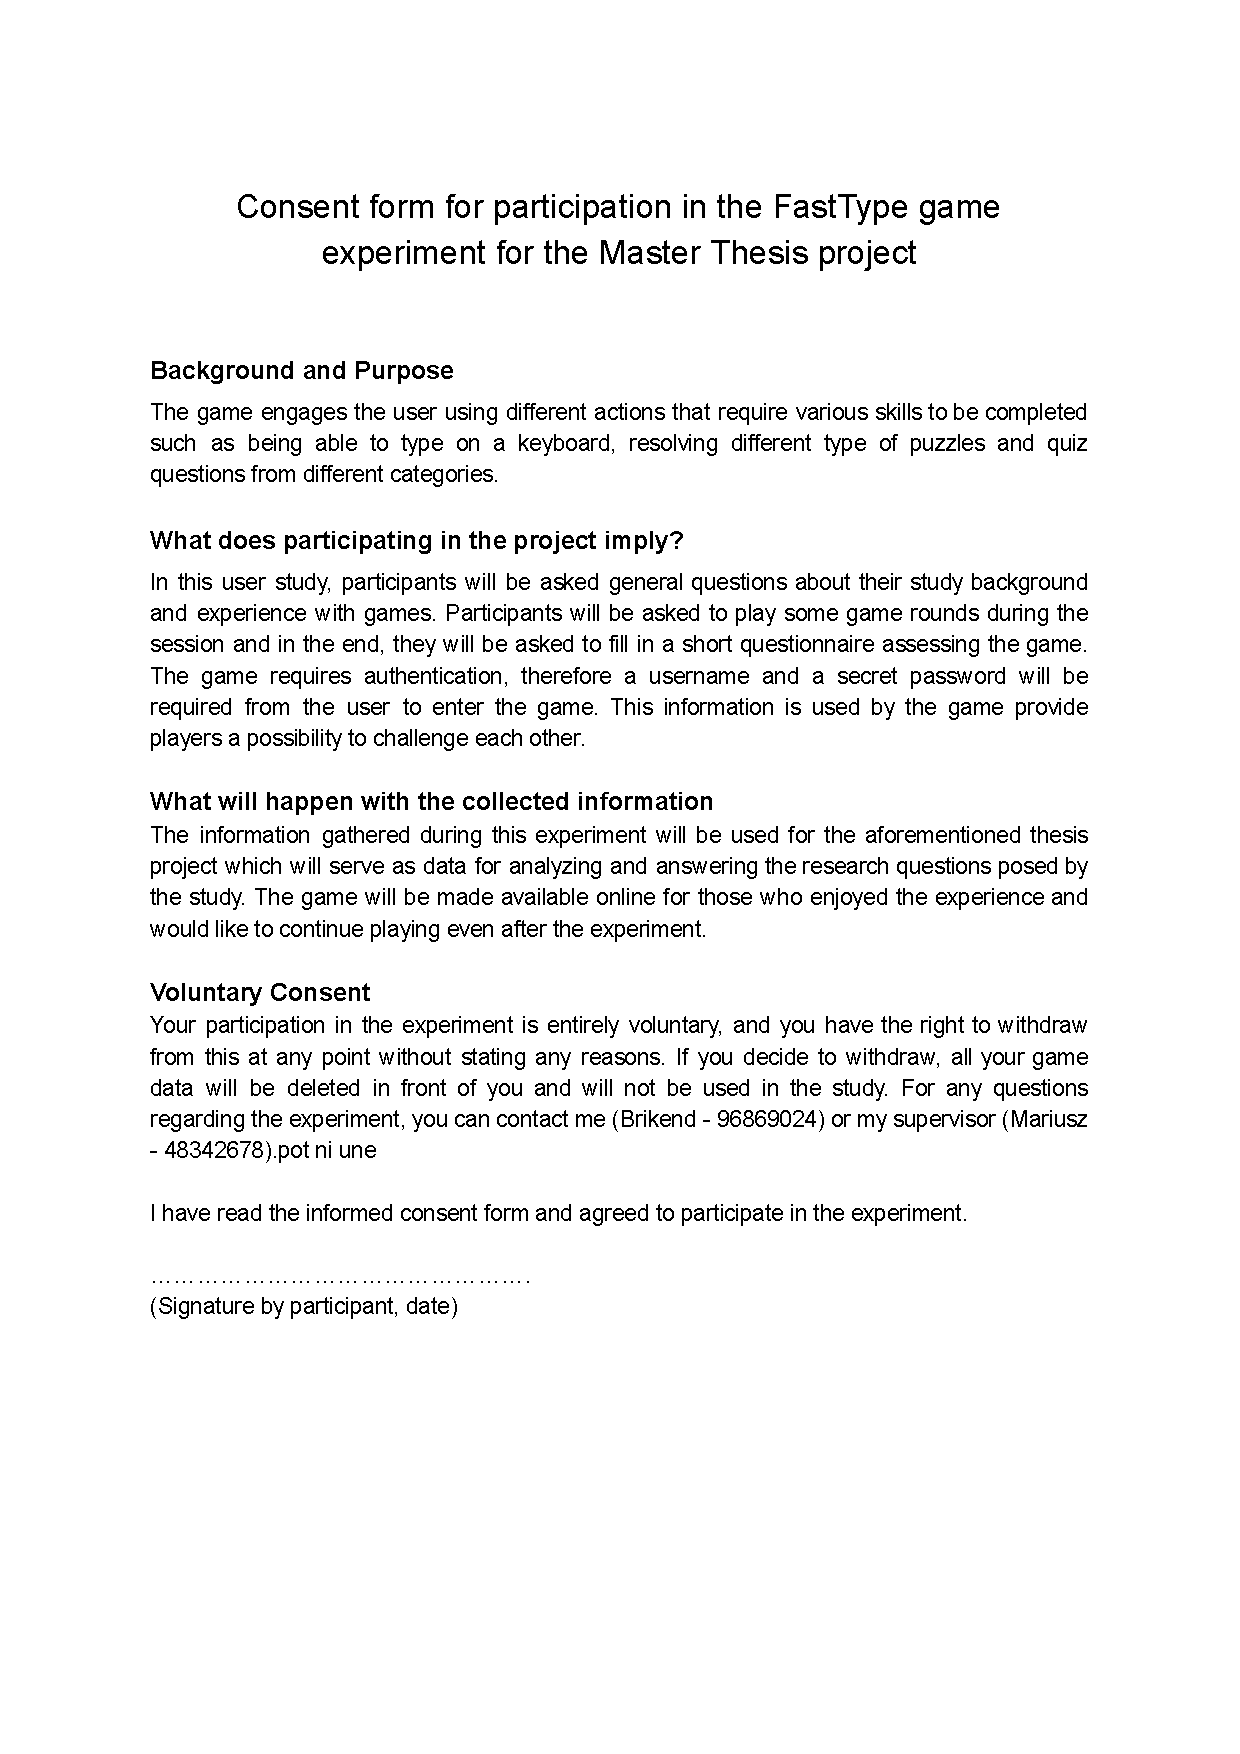
\includepdf[scale=0.8,pages=1,pagecommand=\section{Consent Form}]{appendices/ex2-consentform.pdf}

%Ex1 - Pre Questionnaire
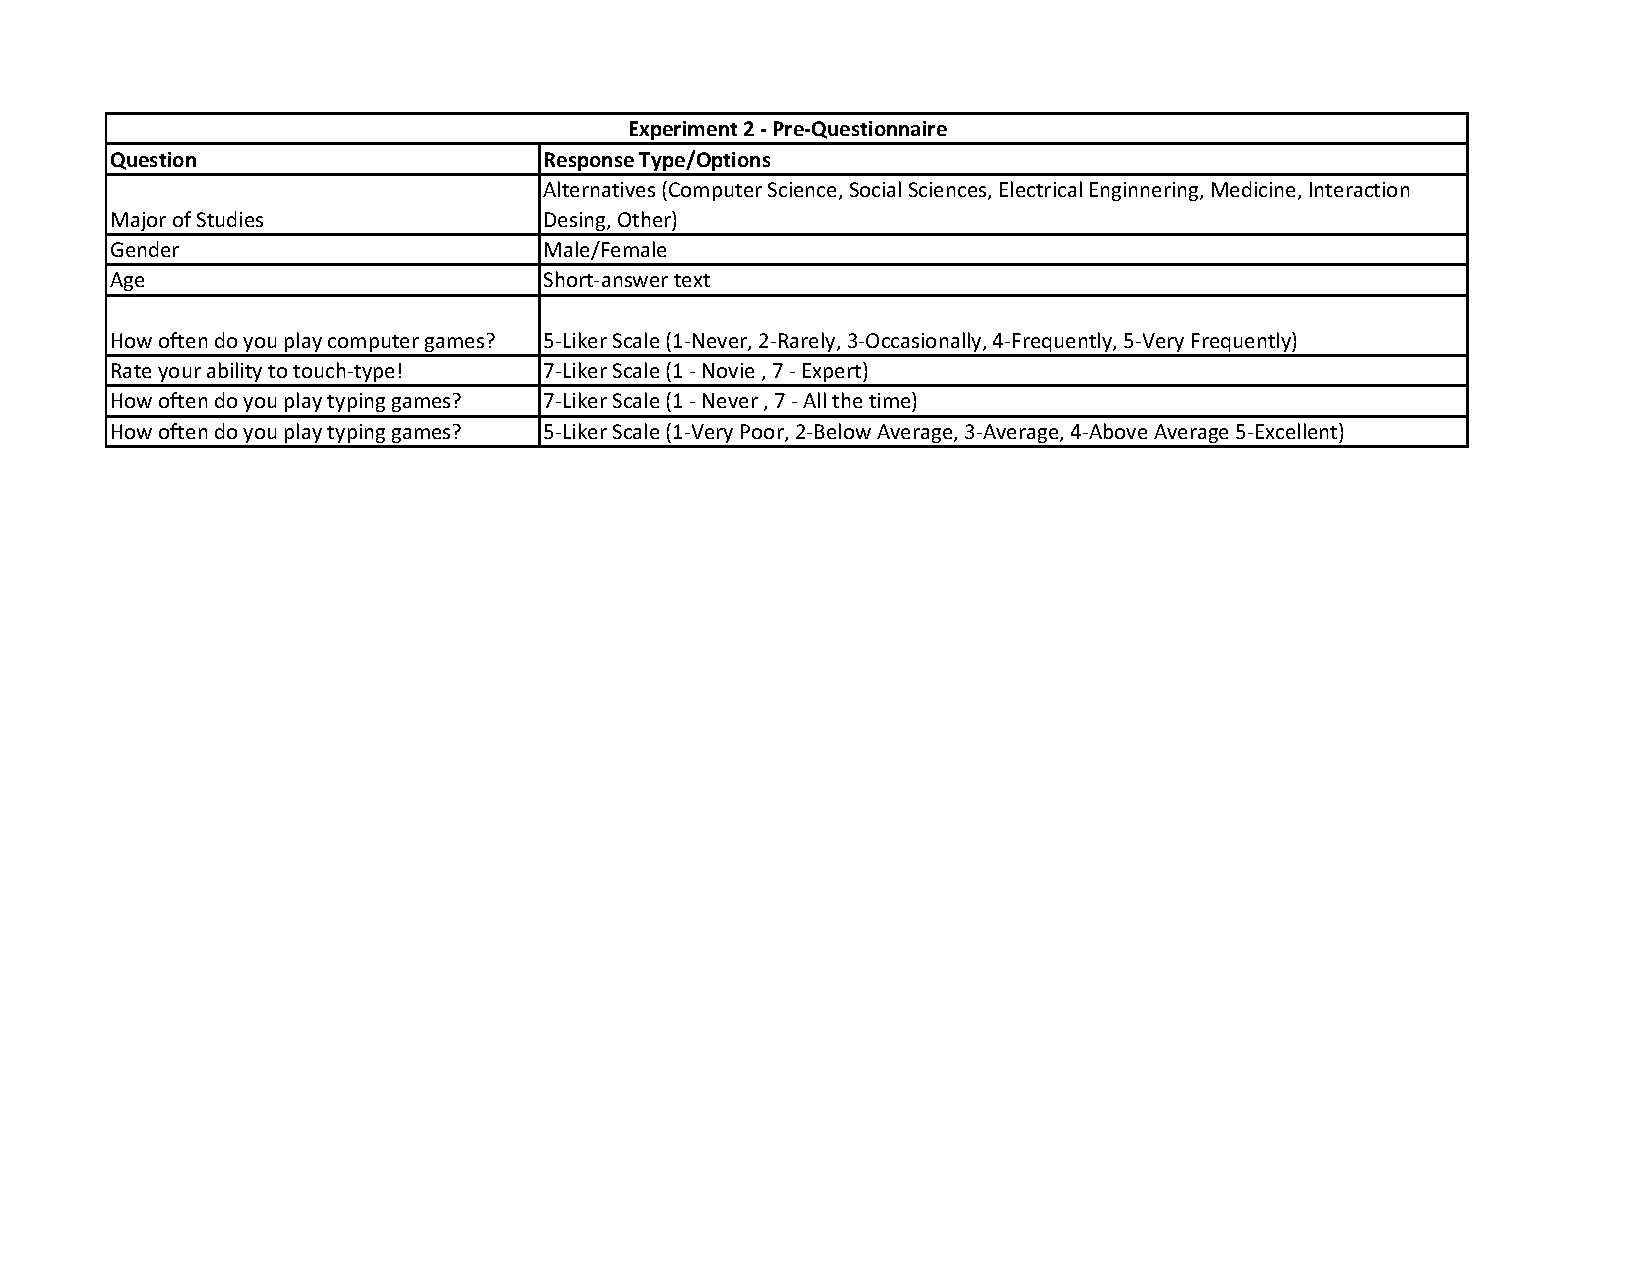
\includepdf[scale=0.8,angle=90,pagecommand=\section{Pre-Questionnaire }]{appendices/ex2-prequestionnaire.pdf}

%Ex2 - Post Questionnaire
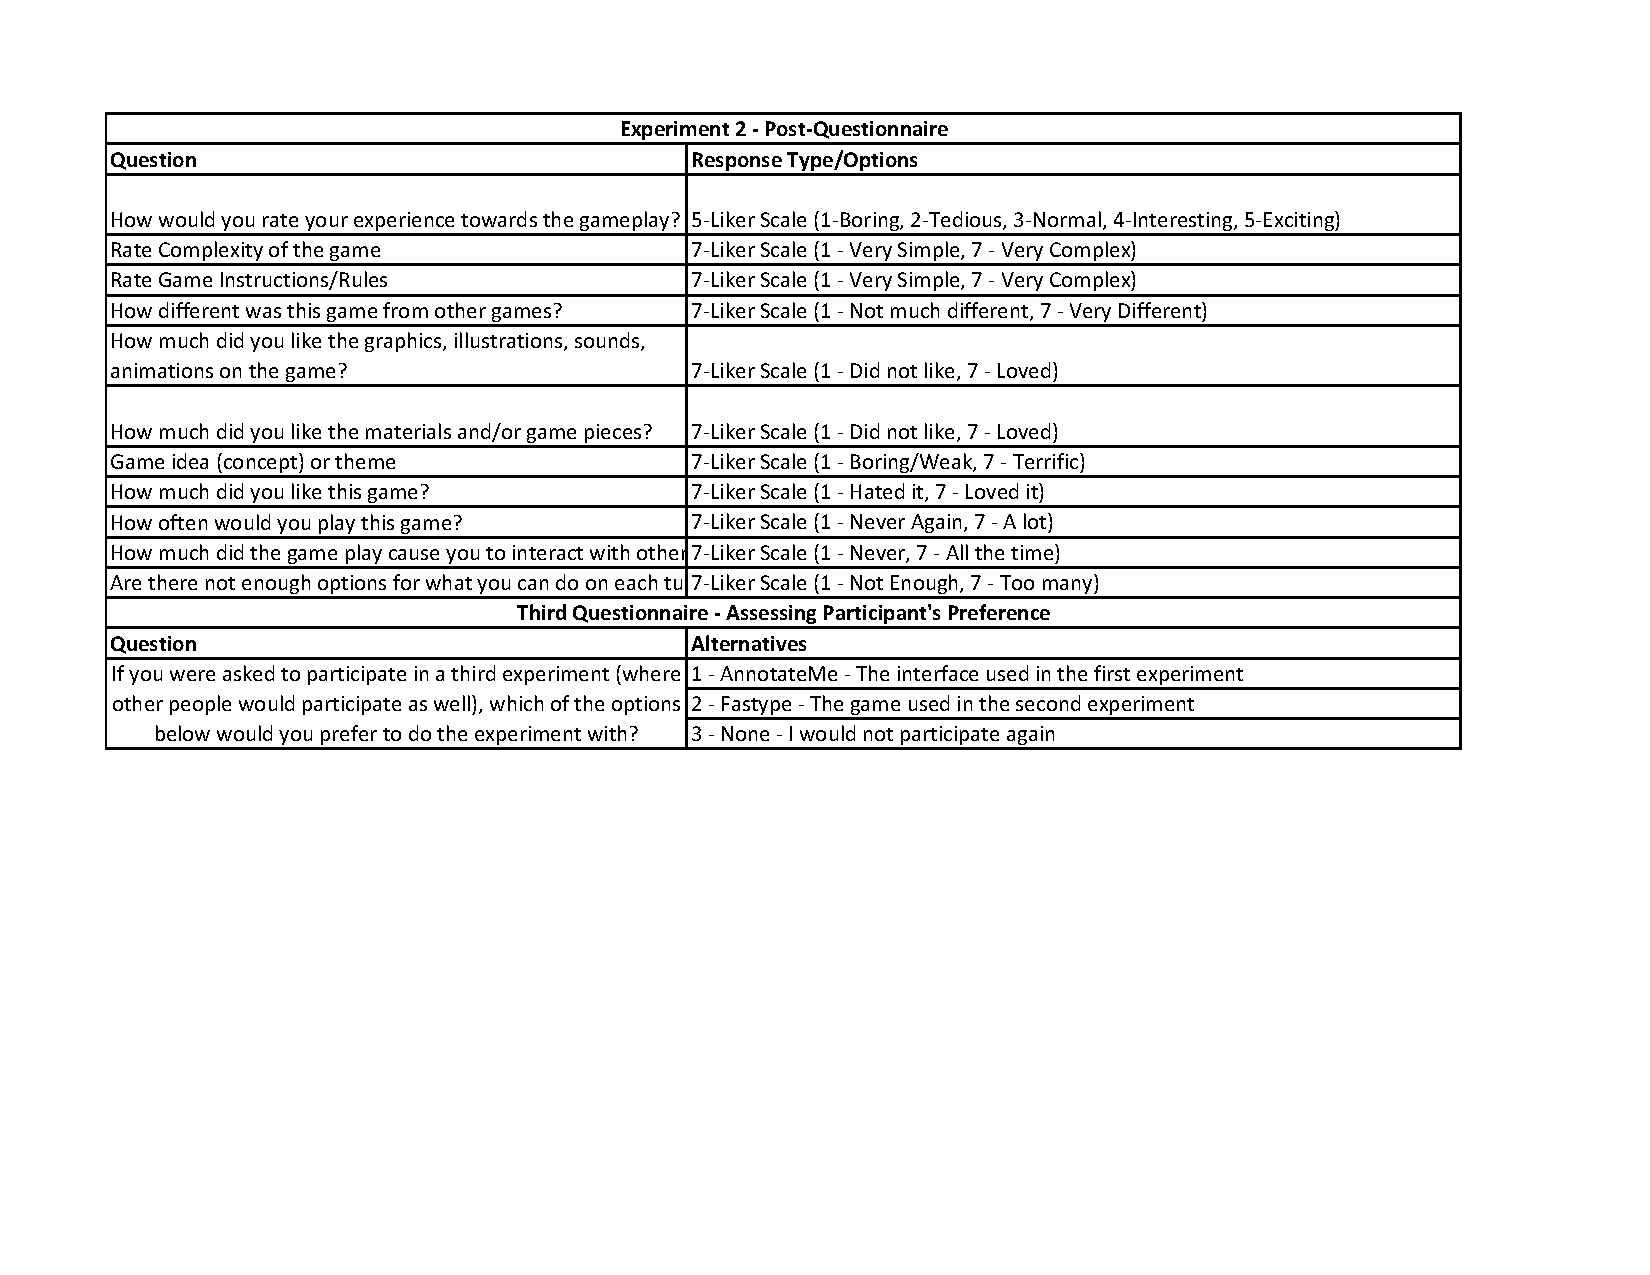
\includepdf[scale=0.8,angle=90,pagecommand=\section{Post-Questionnaire \& Preference Questionnaire }]{appendices/ex2-post-both.pdf}

\chapter{Anova - Raw Data Analysis}
\label{appendix3:chapter}


\section{Attractiveness of Interfaces}
\label{appendix3:attractiveness_analysis}
Below we present the Anova calculations performed on the gathered observations when asked participants about their experience with both interfaces. 

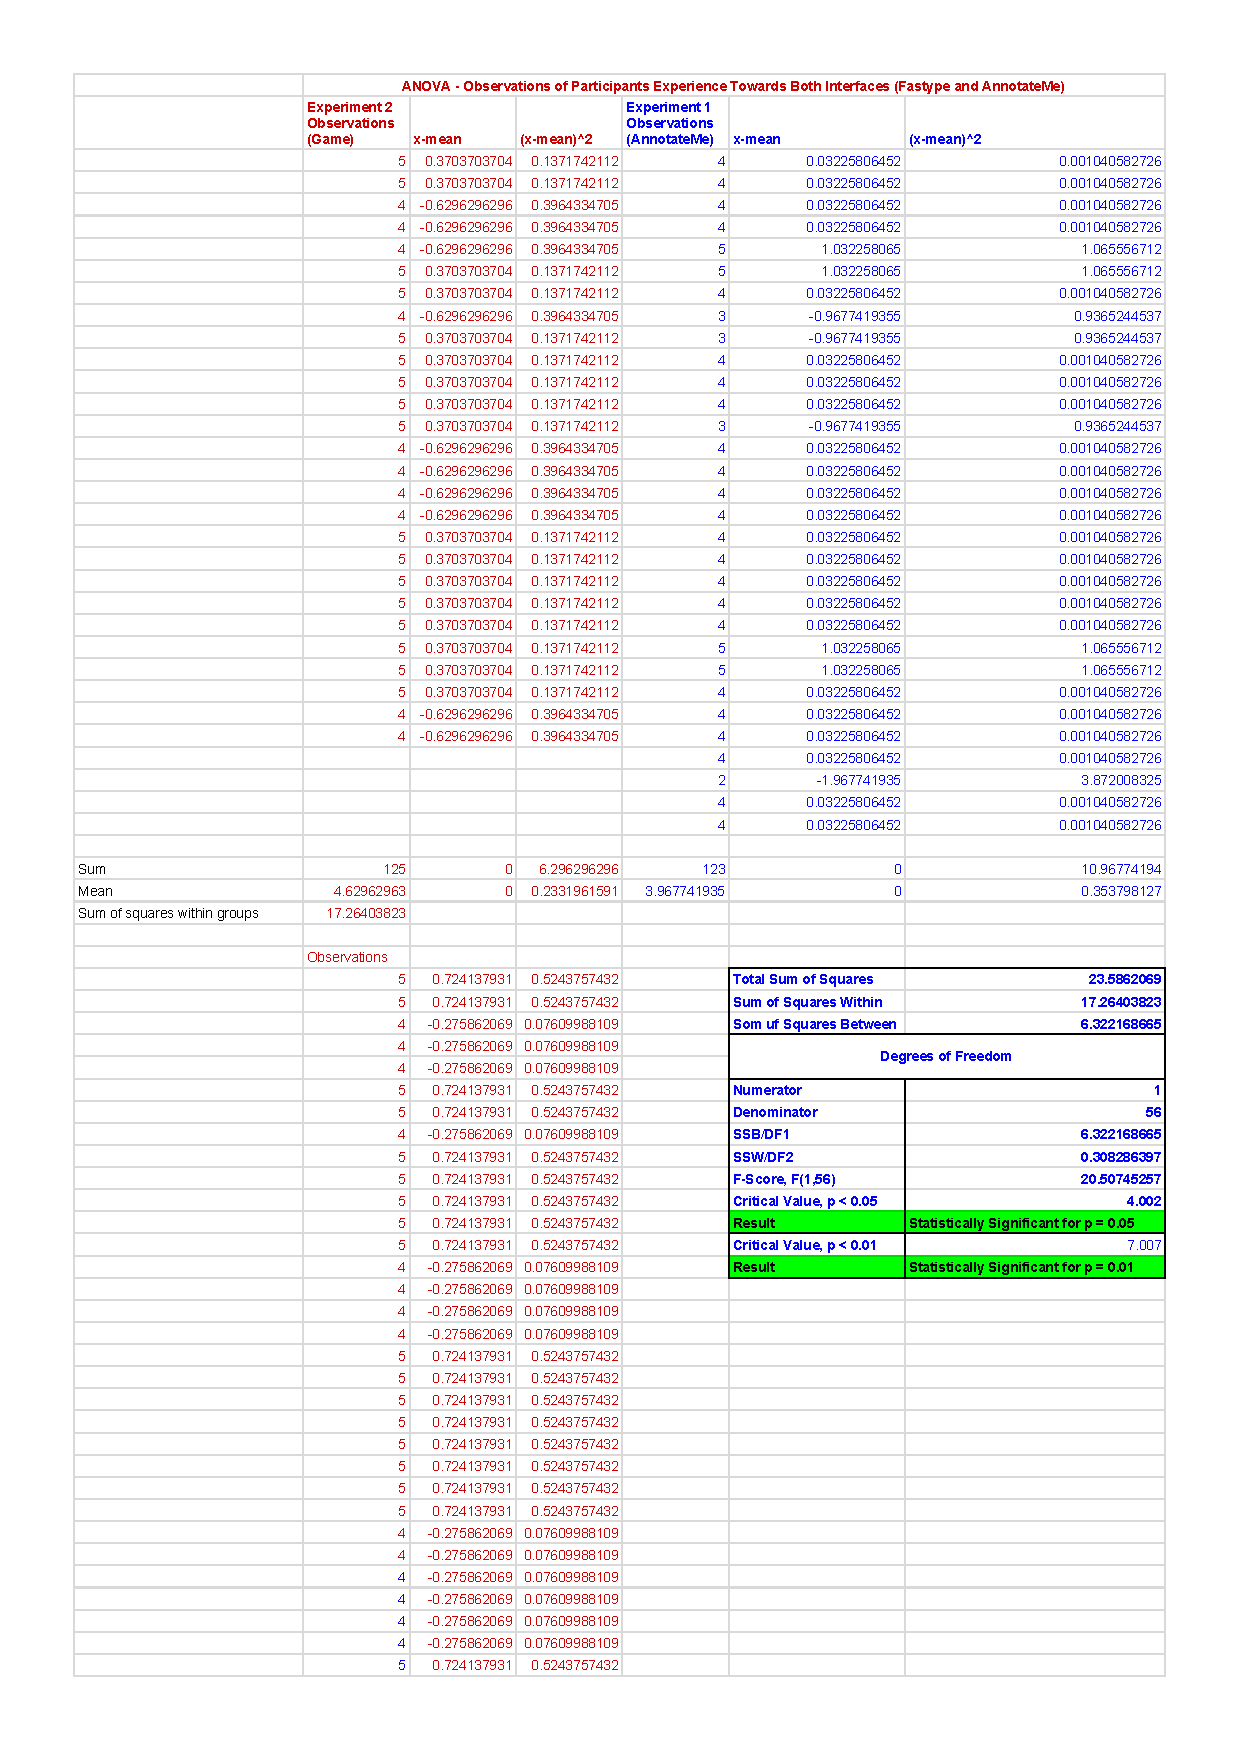
\includepdf[scale=0.7,pages=-]{appendices/anova-participant-experince.pdf}

\section{Player Engagement Analysis}
\label{appendix3:engagement_analysis}
The analysis presented below represent the Anova analysis performed on the gathered observations when participants where asked to rate their engagement with both interfaces using a liker-scale measure\footnote{For the first experiment we used 5-liker scale whereas for the second experiment we used a 7-liker scale. We normalize the observations afterwards to accurately perform comparison measures}. Please note that different measure metrices were used in each experiment, however, a normalization procedure is performed for the game observation to scale the values down from a 7-liker scale to 5. 

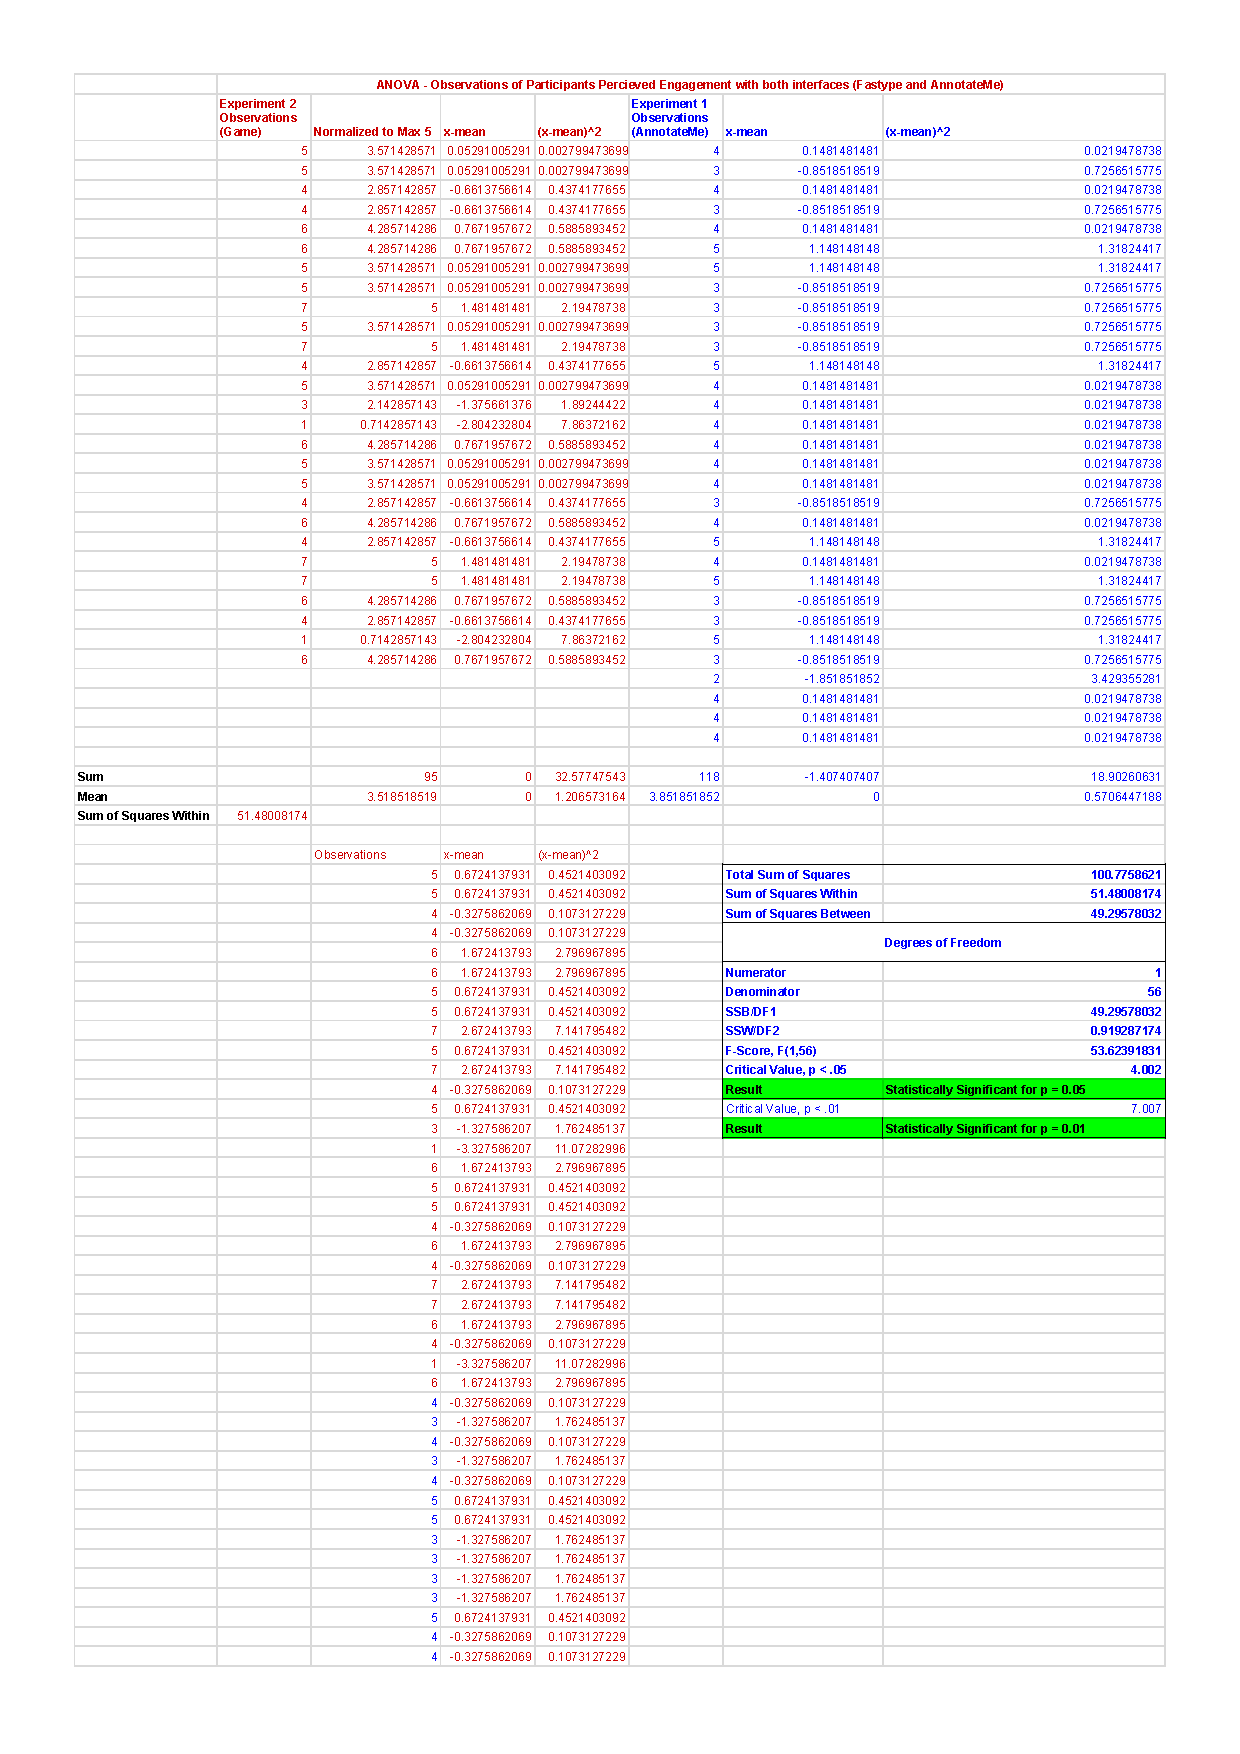
\includepdf[scale=0.7,pages=-]{appendices/participant-engagement.pdf}


\end{document}
